\documentclass[conf]{new-aiaa}
%\documentclass[journal]{new-aiaa} for journal papers
\usepackage[utf8]{inputenc}

\usepackage{graphicx}
\usepackage{amsmath}
\usepackage[version=4]{mhchem}
\usepackage{siunitx}
\usepackage{longtable,tabularx}
\setlength\LTleft{0pt} 
\usepackage{nomencl}
\usepackage{trimclip} % for AR symbol
\usepackage[paper=portrait,pagesize,DIV=13]{typearea}


\usepackage{amsmath,amssymb,url,subfigure,graphicx,theorem}
%\usepackage{graphicx,subfigure,hyperref}
%\usepackage{color,comment,algpseudocode,cases}
%\usepackage{amssymb,amsmath,amsthm,graphicx,subfigure}
\usepackage{algpseudocode,cases,booktabs,multirow}
\usepackage{tikz}
\usetikzlibrary{arrows.meta}
\usetikzlibrary{arrows}

\def\AR{\text{\itshape\clipbox{0pt 0pt .32em 0pt}\AE\kern-.30emR}}
\newcommand{\rot}{\ensuremath{\mathrm{rot}}}

\newcommand{\norm}[1]{\ensuremath{\left\| #1 \right\|}}
\newcommand{\bracket}[1]{\ensuremath{\left[ #1 \right]}}
\newcommand{\braces}[1]{\ensuremath{\left\{ #1 \right\}}}
\newcommand{\parenth}[1]{\ensuremath{\left( #1 \right)}}
\newcommand{\pair}[1]{\ensuremath{\langle #1 \rangle}}
\newcommand{\met}[1]{\ensuremath{\langle\langle #1 \rangle\rangle}}
\newcommand{\refeqn}[1]{(\ref{eqn:#1})}
\newcommand{\reffig}[1]{Figure \ref{fig:#1}}
\newcommand{\tr}[1]{\mathrm{tr}\ensuremath{\negthickspace\bracket{#1}}}
\newcommand{\trs}[1]{\mathrm{tr}\ensuremath{[#1]}}
\newcommand{\ave}[1]{\mathrm{E}\ensuremath{[#1]}}
\newcommand{\deriv}[2]{\ensuremath{\frac{\partial #1}{\partial #2}}}
\newcommand{\dderiv}[2]{\ensuremath{\dfrac{\partial #1}{\partial #2}}}
\newcommand{\SO}{\ensuremath{\operatorname{SO(3)}}}
\newcommand{\T}{\ensuremath{\mathsf{T}}}
\renewcommand{\L}{\ensuremath{\mathsf{L}}}
\newcommand{\so}{\ensuremath{\mathfrak{so}(3)}}
\newcommand{\SE}{\ensuremath{\mathsf{SE(3)}}}
\newcommand{\se}{\ensuremath{\mathfrak{se}(3)}}
\renewcommand{\Re}{\ensuremath{\mathbb{R}}}
\newcommand{\aSE}[2]{\ensuremath{\begin{bmatrix}#1&#2\\0&1\end{bmatrix}}}
\newcommand{\ase}[2]{\ensuremath{\begin{bmatrix}#1&#2\\0&0\end{bmatrix}}}
\newcommand{\D}{\ensuremath{\mathbf{D}}}
\renewcommand{\d}{\ensuremath{\mathfrak{d}}}
\newcommand{\Sph}{\ensuremath{\mathsf{S}}}
\renewcommand{\S}{\Sph}
\newcommand{\J}{\ensuremath{\mathbf{J}}}
\newcommand{\Ad}{\ensuremath{\mathrm{Ad}}}
\newcommand{\ad}{\ensuremath{\mathrm{ad}}}
\newcommand{\intp}{\ensuremath{\mathbf{i}}}
\newcommand{\extd}{\ensuremath{\mathbf{d}}}
\newcommand{\hor}{\ensuremath{\mathrm{hor}}}
\newcommand{\ver}{\ensuremath{\mathrm{ver}}}
\newcommand{\dyn}{\ensuremath{\mathrm{dyn}}}
\newcommand{\geo}{\ensuremath{\mathrm{geo}}}
\newcommand{\Q}{\ensuremath{\mathsf{Q}}}
\newcommand{\G}{\ensuremath{\mathsf{G}}}
\newcommand{\g}{\ensuremath{\mathfrak{g}}}
\newcommand{\Hess}{\ensuremath{\mathrm{Hess}}}

\newcommand{\bfi}{\bfseries\itshape\selectfont}
\DeclareMathOperator*{\argmax}{arg\,max}
\DeclareMathOperator*{\argmin}{arg\,min}

\graphicspath{{"/Users/tylee/Documents/Research/Flapping Wing/doc/Figs/"},{./Figs/}}

\newtheorem{lemma}{Lemma}
\newtheorem{assumption}{Assumption}
\newtheorem{theorem}{Theorem}
\newtheorem{definition}{Definition}

\newtheorem{remark}{Remark}
\newtheorem{prop}{Proposition}
\newenvironment{proof}{\paragraph{Proof:}}{\hfill$\square$}

\title{Dynamic Effects of Abdomen Undulation in the Flight of Monarch Butterfly}

\author{Madhu Sridhar,\footnote{Graduate Student, Mechanical and Aerospace Engineering, University of Alabama Huntsville, 301 Sparkman Dr, Huntsville AL 35899}
Chang-kwon Kang\footnote{Assistant Professor, Mechanical and Aerospace Engineering, University of Alabama Huntsville, 301 Sparkman Dr, Huntsville AL 35899}}
\affil{University of Alabama Huntsville, Huntsville AL, 35899}
\author{Taeyoung Lee\footnote{Associate Professor, Mechanical and Aerospace Engineering, The George Washington University, 800 22nd st NW, Washington DC, 20052.}}
\affil{The George Washington University, Washington DC, 20052}
 
\begin{document}

\maketitle

\begin{abstract}
    This paper presents a geometric formulation of the dynamics of a flapping wing aerial vehicle and utilize it to study the flight dynamics of a Monarch butterfly. 
    The proposed model is essentially articulated rigid bodies, where two wings and an abdomen are connected to a thorax via spherical joint.
    An intrinsic form of Lagrangian mechanics is developed to study the inertial effects of the relative rotation between each part. 
    Next, a quasi-steady aerodynamic model is presented without relying on the common assumption that the flapping frequency is sufficiently large. 
    Consequently, it is suitable to study the flight of a butterfly that is characterized by a relatively large wings flapping in a lower frequency. 
    The outcome of the proposed model is compared with the captured motion of a live Monarch butterfly.
    It is shown that the undulation of the abdomen increases the climb rate and the forward velocity.
\end{abstract}

%\section{Nomenclature}

%{\renewcommand\arraystretch{1.0}
%\noindent\begin{longtable*}{@{}l @{\quad=\quad} l@{}}
    %ECI & Earth-centered inertial frame\\
    %ECEF & Eather-centered, Earth-fixed frame\\
    %$\SO$  & special orthogonal group, $\{R\in\Re^{3\times 3}\,|\, R^TR=I_{3\times 3},\;\mathrm{det}[R]=1\}$\\
    %$\Sph^2$ & unit-sphere, $\Sph^2=\{q\in\Re^3\,|\, \|q\|=1\}$\\
    %$R\in\SO$ & attitude of the spacecraft, \\
              %& linear transformation from the body-fixed frame to the Earth-centered inertial frame\\
    %$\Omega\in\Re^3$ & angular velocity of the spacecraft, resolved in the body-fixed frame\\
    %$F\in\Re^{3\times 3}$ & parameter of the matrix Fisher distribution\\
    %$c(F)\in\Re$ & normalizing constant of the matrix Fisher distribution with the parameter $F$\\
    %$b\in\Sph^2$ & the direction of the Earth magnetic field in the ECEF frame
%\end{longtable*}}

\section{Introduction}

The Monarch butterfly is one of the most popular butterfly species in North America with wings of around 4 cm featuring an easily recognizable black, orange, and white pattern.
They exhibit remarkable flight characteristics \cite{Brower1977}, migrating annually from North America to Mexico - up to 4000 km \cite{Brower1996,Masters1988,Merlin}, the longest flight range among insects \cite{Gibo1981,Brower1996,Nin2013,Templin2000}.
However, the physical mechanism enabling this long-range flight is not well understood.
One theory is that the Monarchs benefit from their high-altitude flight.
Monarchs butterflies fly at high-altitudes during migration ({\raise.17ex\hbox{$\scriptstyle\sim$}}1,250m) and overwinter ({\raise.17ex\hbox{$\scriptstyle\sim$}}3,000m) at high altitudes.
At these altitudes, they can take advantage of the boundary layer of the earth to conserve energy.
Furthermore, aerodynamic drag is proportional to air density, which decreases with altitude.
A minimal aerodynamic drag is critical to enable the long-range migration, which is provided by flying at high altitudes.
However, the lift is also expected to decrease with lower density at higher altitudes.
Unlike airplanes, Monarchs must generate the propulsive forces with their flapping motion.
How butterflies efficiently generate lift and fly during migration is one of the unsolved mysteries.

Compared to the wealth of research on the flight of insects such as flies \cite{Dickinson1999b,Muijres2014}, bees \cite{Dillon2014,Mountcastle2013}, dragonflies \cite{Wang2005c,Jongerius2010,Wang2007,Alexander1984,Wang2005h}, or birds and bats \cite{Shyy2013}, butterfly flight remains inadequately understood due to their many unique characteristics.
Unlike most insects, the fore and hindwings of butterflies are relatively large and move in sync \cite{Betts1988}.
Butterflies are extremely evasive with agile maneuvers \cite{Dudley1991,Thomas2004a,Srygley1994,Dudley1994} and body undulations with closely coupled wing-body interaction \cite{Srygley1994,Lin2012,kang2017aiaaj}.
In particular, the butterfly body exhibits considerable vertical oscillation during flight due to the instantaneous change in wing shape and inertia \cite{Tanaka2010,Lin2012}, resulting in a ``bumpy'' flight trajectory.
Flapping wings and body move in unison as reported in our earlier work \cite{kang2017aiaaj}, suggesting that the butterfly flight is an outcome of closely coupled wing-body interaction.

The main obstacle in discovering the long-range flight mechanisms in the Monarch flight is this highly coupled dynamics of the slowly flapping motion and the body.
The large wings continuously rotate during flight, which is also affected by the body dynamics.
Furthermore, the thorax of the Monarchs continuously pitches while their abdomen moves relative to the thorax during flight.
As a consequence, most flight dynamic equations of motion and control schemes that have been derived in the literature cannot be used to study the butterfly flight.
The conventional models exploit the large disparity in the time scales of wingbeat frequency and body dynamics assuming smaller insects such as fruit flies and bumblebees~\cite{Elzinga2015,Taha2012}.
Furthermore, many flapping wing dynamics models are based on the common simplified formulation where the nonlinear time-varying flapping dynamics are transformed into linear time-invariant systems by considering small perturbations averaged over the period of flapping~\cite{Schenato2003,Deng2006,Doman2010,Shyy}.
These approaches are not suitable to analyze the low-frequency flapping dynamics of Monarch butterflies. 

A key open research question associated with the butterfly flight is the effects of dynamics on the power consumption.
Whereas the pitching motion of smaller flying insects play a critical role in aerodynamic force generation ~\cite{Dickinson1999b,Shyy2013}, most butterfly wings are structurally restricted from pitching ~\cite{Tanaka2010}.
Instead, it is presumed that the relatively large aerodynamic forces generated by the simple flapping wing motions affect the body attitude and vertical displacement, which alter the effective angle of attack and, hence, the flapping wing aerodynamics.
As such, by adjusting the center of mass, a butterfly inspired ornithopter without a tail could fly forward passively without a feedback controller ~\cite{Tanaka2010}.
If the foward flight of butterflies were indeed passive, the power consumption is expected to be lower than an actively controlled flight.
The power savings due to coupled wing-body motion can contribute to our understanding of the long-range Monarch migration ~\cite{Sridhar2019}, which, in turn, can inform the development of long-range micro flying robots.
However, there are also reports that butterfly’s flight under periodic flapping motion is unstable because the butterfly cannot maintain its body pitch angle within a proper range ~\cite{Yokoyama2013,Jayakumar2018}.
The motion of the abdomen had to be actively controlled to stabilize the butterfly flight \cite{Jayakumar2018}.

The objective of this paper is to derive, validate, and analyze a butterfly flight dynamics model to study the dynamic and power implication of the Monarch butterfly flight.
We model a flapping wing aerial vehicle as articulated rigid bodies, where two wings and an abdomen are connected to a thorax via spherical joint based on a geometric formulation.
An intrinsic form of Lagrangian mechanics is developed to include and study the inertial effects of the relative rotation between each part.
To model the flapping wing aerodynamics, a quasi-steady blade element model is formulated without relying on the common assumption that the flapping frequency is sufficiently large to study the flight, characterized by relatively large, slowly flapping wings.
The results of this model are compared to the detailed motion of the thorax, abdomen, and the pair of wings of freely flying Monarch butterflies.
The live Monarch butterfly flight is measured using a motion-tracking system \cite{kang2017aiaaj}.
Our preliminary results show that the trajectory of the velocity asymptotically converges to a periodic orbit, suggesting that the flapping motion captured by the Monarch butterfly yields an asymptotically stable periodic solution.
Furthermore, the abdomen undulation increases the climb rate and the forward velocity.


\section{Flapping Wing UAV Model}

Consider a flapping wing UAV that is composed of a head, a thorax, an abdomen, and two wings attached to the thorax. 
Here, we assume that the head and the thorax are coagulated into a single rigid body, which is referred to as \textit{body}. 
We plan to study the motion of the abdomen relative to the thorax in the future. 
Also, we do not distinguish hindwings from forewings. 

Define an inertial frame $\mathcal{F}_I=\{\mathbf{i}_x,\mathbf{i}_y,\mathbf{i}_z\}$, where the third axis points downward, and the first two axes span the horizontal plane. 
This is compatible to the NED (north-east-down) frame common in flight dynamics.
\nomenclature{$\mathcal{F}_I$}{North-East-Down inertial frame}
\nomenclature{$\mathbf{i}_x,\mathbf{i}_y,\mathbf{i}_z$}{basis vector of the inertial frame}

\subsection{Body}

Define the body-fixed frame $\mathcal{F}_B=\{\mathbf{b}_x,\mathbf{b}_y,\mathbf{b}_z\}$,
whose origin is located at its mass center of the body.
Following the common convention in flight dynamics, the first axis points toward the head, the second axis point toward the right wing, and the third axis points toward the ventral (belly) side.
\nomenclature{$\mathcal{F}_B$}{body-fixed frame (see Figure \ref{fig:FI_FB})}
\nomenclature{$\mathbf{b}_x,\mathbf{b}_y,\mathbf{b}_z$}{basis vector of the body-fixed frame}

\setlength{\unitlength}{0.1\columnwidth}
\begin{figure}[h]
    \begin{center}
        \footnotesize
        \begin{picture}(3,3)(0,0)
            \put(0,0){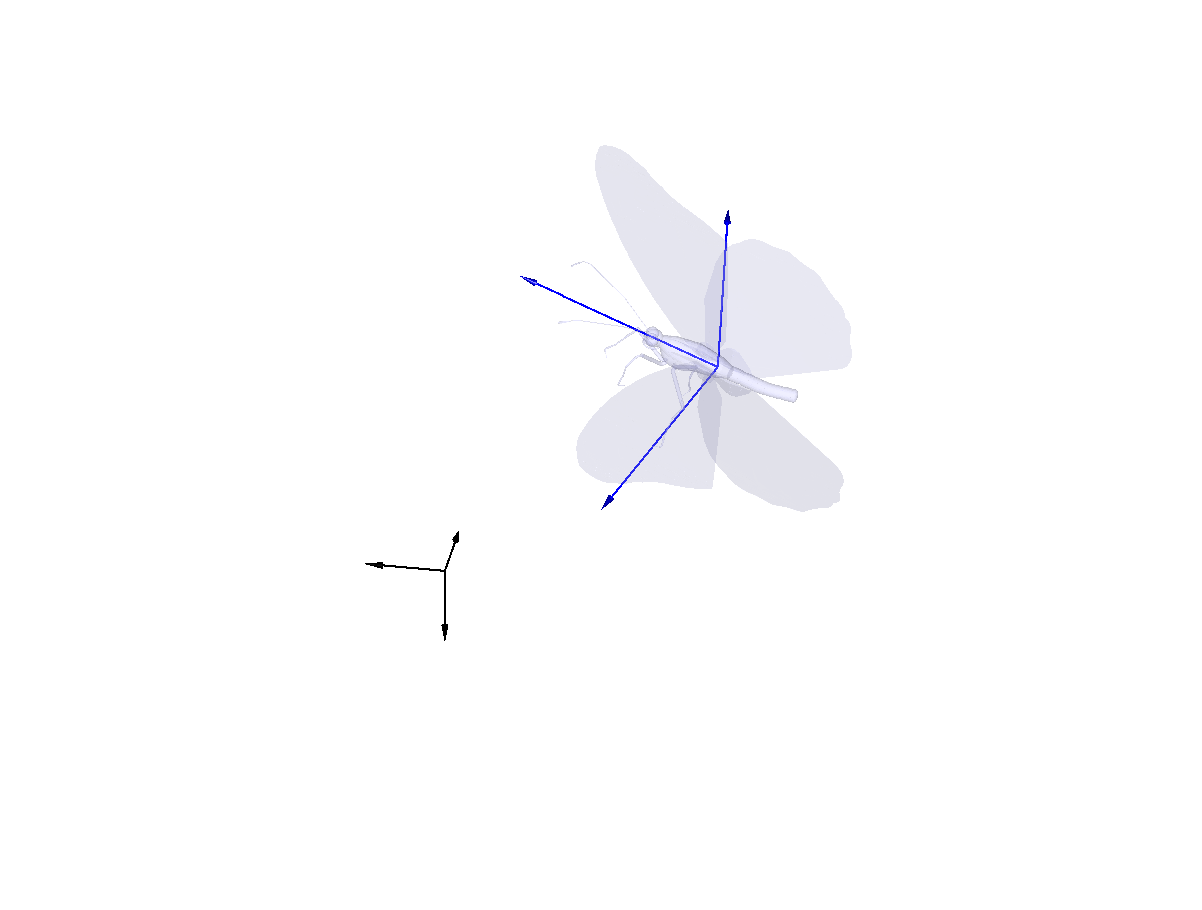
\includegraphics[trim={6cm 4cm 5cm 2cm},clip,width=0.3\textwidth]{monarch_FB}}
            \put(-0.1,0.4){$\mathbf{i}_x$}
            \put(0.55,0.65){$\mathbf{i}_y$}
            \put(0.5,0.05){$\mathbf{i}_z$}
            \put(0.7,2.3){$\mathbf{b}_x$}
            \put(2.1,2.6){$\mathbf{b}_y$}
            \put(1.15,0.7){$\mathbf{b}_z$}
        \end{picture}
    \end{center}
    \caption{The inertial frame $\mathcal{F}_I=\{\mathbf{i}_x,\mathbf{i}_y,\mathbf{i}_z\}$ (black) and the body-fixed frame $\mathcal{F}_B=\{\mathbf{b}_x,\mathbf{b}_y,\mathbf{b}_z\}$ (blue)}\label{fig:FI_FB}
\end{figure}
The location of the mass center is given by $x\in\Re^3$ in $\mathcal{F}_I$. 
The attitude of the body is described by $R\in\SO=\{R\in \Re^{3\times 3}\,|\, R^T R = I_{3\times 3},\; \mathrm{det}[R]=1\}$, which represents the linear transformation of a representation of a vector from $\mathcal{F}_B$ to $\mathcal{F}_I$. 
\nomenclature{$\SO$}{three-dimensional special orthogonal group, $\SO=\{R\in \Re^{3\times 3}\,|\, R^T R = I_{3\times 3},\; \mathrm{det}[R]=1\}$}
\nomenclature{$\so$}{Lie algebra of $\SO$, $\so=\{S\in \Re^{3\times 3}\,|\, S^T=-S\}$}
The attitude kinematics is given by
\begin{align}
    \dot R = R \hat \Omega,
\end{align}
where $\Omega\in\Re^3$ is the angular velocity resolved in $\mathcal{F}_B$. 
In the above equation, the \textit{hat} map $\wedge:\Re^3\rightarrow \so$ is defined such that $\hat x y = x\times y$ for any $x,y\in\Re^3$, or equivalently
\begin{align}
    \hat x = \begin{bmatrix}
        0 & -x_3 & x_2 \\
        x_3 & 0 & -x_1 \\
        -x_2 & x_1 & 0 
    \end{bmatrix},\label{eqn:hat_map}
\end{align}
for $x=(x_1,x_2,x_3)\in\Re^3$. 
The inverse of the hat map is denoted by the \textit{vee} map, $\vee: \so\rightarrow \Re^3$.
\nomenclature{$x\in\Re^3$}{the location of the mass center of the body represented in $\mathcal{F}_I$}
\nomenclature{$R\in\SO$}{the attitude of the body, the linear transformation of the representation of a vector from $\mathcal{F}_B$ to $\mathcal{F}_I$}
\nomenclature{$\Omega\in\Re^3$}{the angular velocity of the body represented in $\mathcal{F}_B$}
\nomenclature{$\wedge$}{the hat map\nomrefeq}
\nomenclature{$\vee$}{the vee map\nomrefeq}


\subsection{Wing}

\paragraph{Right Wing}

Let $\mathcal{F}_R=\{\mathbf{r}_x,\mathbf{r}_y,\mathbf{r}_z\}$ be the frame fixed to the right wing.
Its origin is located at the joint of the right wing, or the wing root where the right wing is attached to the thorax. 
The vector from the origin of $\mathcal{F}_B$ to the origin of $\mathcal{F}_R$ is defined as $\mu_R\in\Re^3$. 
As it is resolved in $\mathcal{F}_B$ and the body is rigid, $\dot\mu_R=0$.
The first two axes of $\mathcal{F}_R$ span the plane of the wing, where the first axis points toward the leading edge and the second axis points toward the wing tip. 
Consequently, the third axis is normal to the wing plane, and it points toward the ventral side when there is no rotation of the right wing.
\nomenclature{$\mathcal{F}_R$}{frame fixed to the right wing (see Figure~\ref{fig:FR})}
\nomenclature{$\mathbf{r}_x,\mathbf{r}_y,\mathbf{r}_z$}{basis vector of $\mathcal{F}_R$}
\nomenclature{$\mu_R\in\Re^3$}{the fixed vector from the mass center of the body to the root of the right wing resolved in $\mathcal{F}_B$}

\setlength{\unitlength}{0.1\columnwidth}
\begin{figure}[h]
    \begin{center}
        \footnotesize
        \begin{picture}(3,2.4)(0,0)
           \put(0,0){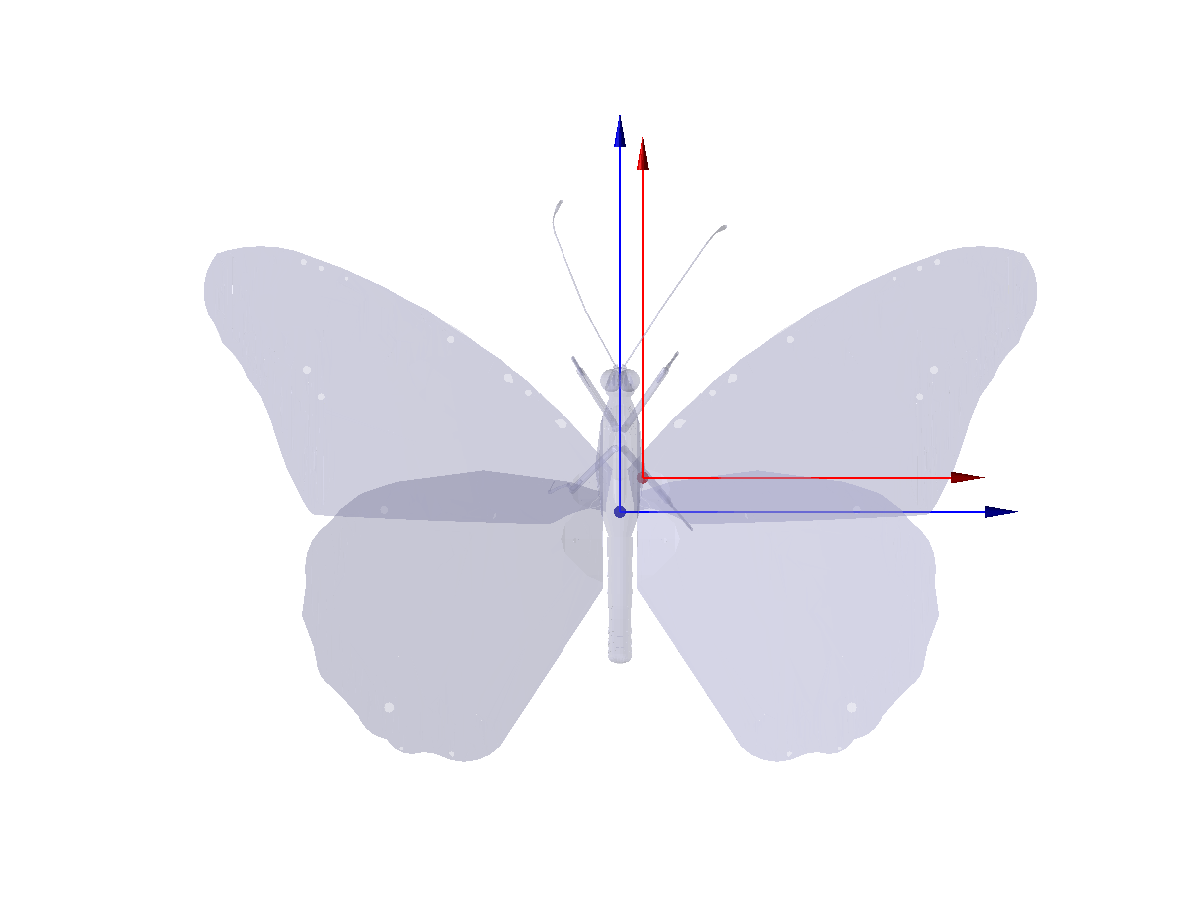
\includegraphics[trim={3cm 2cm 2cm 1cm},clip,width=0.3\textwidth]{monarch_FR}}
           \put(1.6,2.2){$\mathbf{r}_x$}
           \put(1.2,2.25){$\mathbf{b}_x$}
           \put(2.7,1.1){$\mathbf{r}_y$}
           \put(2.85,0.75){$\mathbf{b}_y$}
        \end{picture}
    \end{center}
    \caption{The body-fixed frame $\mathcal{F}_B=\{\mathbf{b}_x,\mathbf{b}_y,\mathbf{b}_z\}$ (blue), the right wing frame $\mathcal{F}_R=\{\mathbf{r}_x,\mathbf{r}_y,\mathbf{r}_z\}$ (red)}\label{fig:FR}
\end{figure}

Next, we introduce the stroke frame $\mathcal{F}_S=\{\mathbf{s}_x,\mathbf{s}_y,\mathbf{s}_z\}$, which is constructed by translating the origin of $\mathcal{F}_B$ to the center of the left wing root and the right wing root, and rotating it about $\mathbf{b}_y$ by $\beta\in[-\pi,\pi)$.
The $y$--$z$ plane of $\mathcal{F}_S$ is referred to as the stroke plane. 

\setlength{\unitlength}{0.1\columnwidth}
\begin{figure}[h]
    \begin{center}
        \footnotesize
        \begin{picture}(3,2.6)(0,0)
           \put(0,0){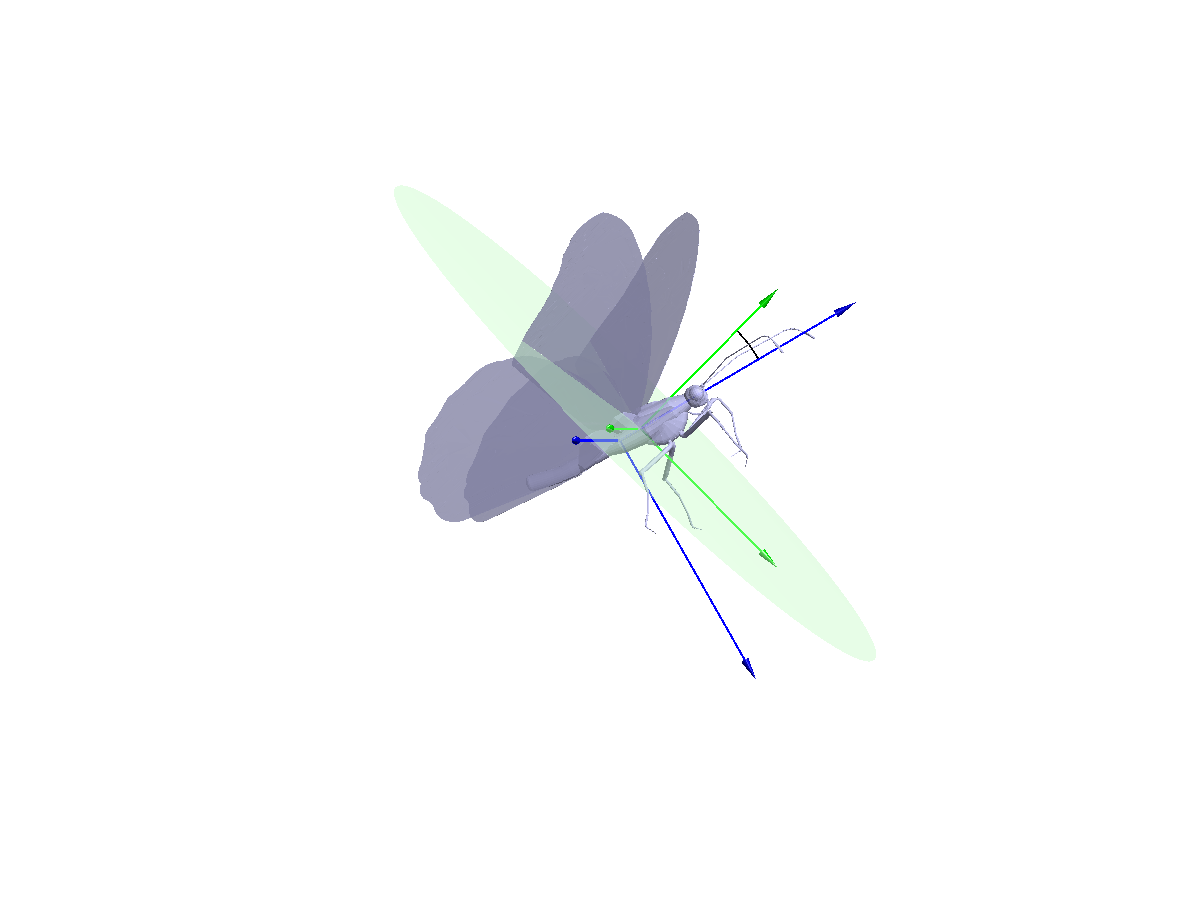
\includegraphics[trim={5cm 3cm 3cm 2cm},clip,width=0.3\textwidth]{monarch_FS}}
           \put(1.95,2.0){$\mathbf{s}_x$}
           \put(2.5,1.95){$\mathbf{b}_x$}
           \put(2.2,0.45){$\mathbf{s}_z$}
           \put(2.05,-0.05){$\mathbf{b}_z$}
           \put(2.05,1.7){$\beta>0$}
           \put(0.05,1.9){\shortstack[c]{stroke\\plane}}
        \end{picture}
    \end{center}
    \caption{The body-fixed frame $\mathcal{F}_B=\{\mathbf{b}_x,\mathbf{b}_y,\mathbf{b}_z\}$ (blue), the stroke frame $\mathcal{F}_S=\{\mathbf{s}_x,\mathbf{s}_y,\mathbf{s}_z\}$ (green)}\label{fig:FS}
\end{figure}

The angle $\beta$ can be considered as the angle between $\mathbf{b}_x$, and $\mathbf{s}_x$ that is normal to the stroke plane. 
Or equivalently, it is the angle between $y$--$z$ plane of $\mathcal{F}_B$ and the stroke plane.
It is positive when $\mathbf{s}_x\cdot \mathbf{b}_z <0$.  
This angle is often defined as the angle between the ground, horizontal plane and the stroke plane, considering hovering flights with a fixed attitude of the body.
Here, it is defined relative to $\mathcal{F}_B$ as the flapping motion is inherently relative to the body. 
\nomenclature{$\mathcal{F}_S$}{stroke frame (see Figure \ref{fig:FS})}
\nomenclature{$\mathbf{s}_x,\mathbf{s}_y,\mathbf{s}_z$}{basis vector of $\mathcal{F}_S$}
\nomenclature{$\beta\in[-\pi,\pi)$}{the angle between $\mathbf{b}_x$ and $\mathbf{s}_x$ that is normal to the stroke plane, or equivalently, the angle between $y$--$z$ plane of $\mathcal{F}_B$ and the stroke plane.
It is positive when $\mathbf{s}_x\cdot \mathbf{b}_z <0$.  (see Figure \ref{fig:FS})}

\begin{figure}
    \centerline{
        \footnotesize
        \subfigure[flapping angle]{
        \begin{picture}(3,2.6)(0,0)
           \put(0,0){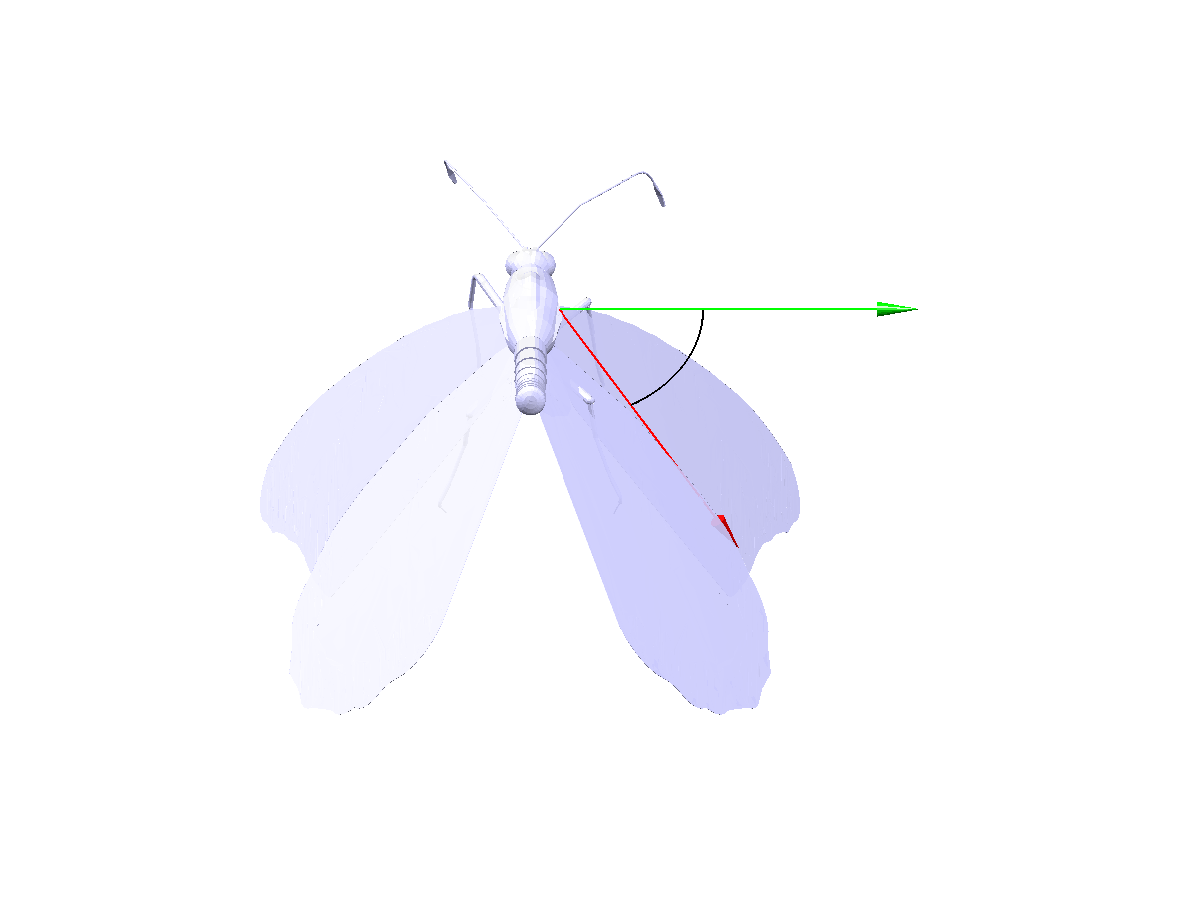
\includegraphics[trim={4cm 3cm 4cm 1.5cm},clip,width=0.3\textwidth]{monarch_FR_phi}}
           \put(1.9,1.4){$\phi>0$}
           \put(2.75,1.9){$\mathbf{s}_y$}
           \put(2.2,0.6){$\mathbf{r}_y$}
        \end{picture}
    }
        \subfigure[pitch angle]{
        \begin{picture}(3,2.6)(0,0)
           \put(0,0){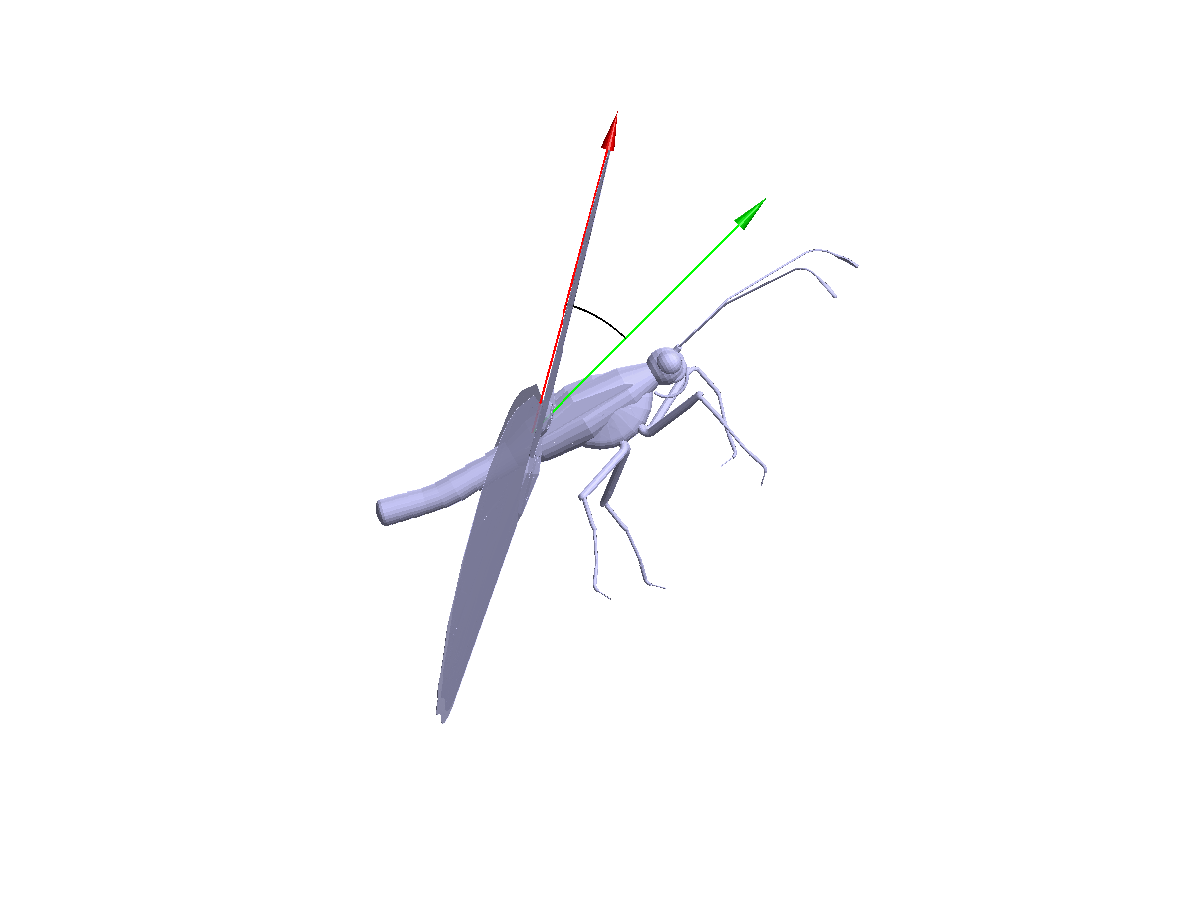
\includegraphics[trim={4cm 3cm 2.5cm 1.5cm},clip,width=0.3\textwidth]{monarch_FR_theta}}
           \put(1.3,1.7){$\theta>0$}
           \put(1.1,2.3){$\mathbf{r}_x$}
           \put(2.0,1.85){$\mathbf{s}_x$}
        \end{picture}
    }
        \subfigure[deviation angle]{
        \begin{picture}(3,2.6)(0,0)
           \put(0,0){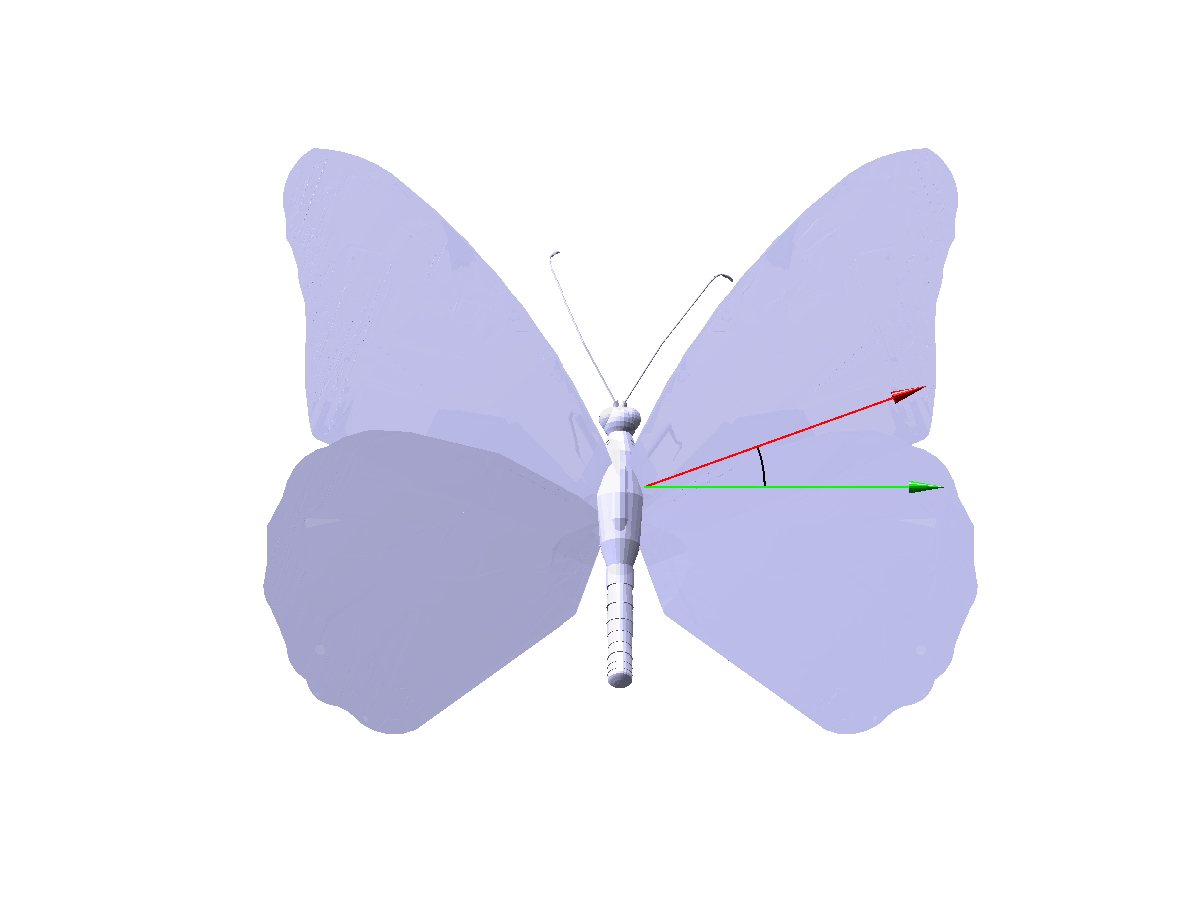
\includegraphics[trim={3cm 2cm 3cm 2cm},clip,width=0.3\textwidth]{monarch_FR_psi}}
           \put(1.8,1.3){$\psi>0$}
           \put(2.8,1.4){$\mathbf{r}_y$}
           \put(2.8,0.95){$\mathbf{s}_y$}
        \end{picture}
    }
}
\caption{Wing configuration when only one of $(\phi,\theta,\psi)$ is non-zero}\label{fig:wing_Euler}
\end{figure}


The motion of the right wing relative to $\mathcal{F}_S$ is described by 1--3--2 Euler angles $(\phi_R,\psi_R,\theta_R)$. 
Consequently, the orientation of the right wing relative to $\mathcal{F}_B$, namely $Q_R\in\SO$ is described by
\begin{align}
    Q_R(t) = \exp(\beta \hat e_2)\exp(\phi_R(t) \hat e_1) \exp(-\psi_R(t) \hat e_3) \exp(\theta_R(t) \hat e_2),\label{eqn:Q_R}
\end{align}
which is the linear transformation of a representation of a vector from $\mathcal{F}_R$ to $\mathcal{F}_B$. 
The Euler-angles are defined as
\begin{itemize}[leftmargin=2.5cm]
    \item[$\phi_R\in[-\pi,\pi)$] the flapping angle, which is positive when the wing is in the ventral side, i.e., $\dot\phi>0$ corresponds to downstroke and $\dot\phi<0$ corresponds to upstroke (this is also referred to as the stroke angle or the sweep angle in other papers)
    \item[$\theta_R\in[-\pi,\pi)$] the pitch angle about the axis from the wing root to the wing tip, which is positive when the leading edge of the wing is rotated toward the dorsal side (this is also referred to as the feathering angle or the rotation angle in other papers)
    \item[$\psi_R\in[-\pi,\pi)$] the deviation angle that governs the motion of the wing tip out of the stroke plane, which is positive when the wing tip is rotated toward the head 
\end{itemize}
\nomenclature{$Q_R\in\SO$}{the attitude of the right wing,  the linear transformation of the representation of a vector from $\mathcal{F}_R$ to $\mathcal{F}_B$}
\nomenclature{$\phi\in[-\pi,\pi)$}{flapping angle (see Figure \ref{fig:wing_Euler})}
\nomenclature{$\theta\in[-\pi,\pi)$}{pitch angle (see Figure \ref{fig:wing_Euler})}
\nomenclature{$\psi\in[-\pi,\pi)$}{deviation angle (see Figure \ref{fig:wing_Euler})}


The time-derivative of $Q_R$ is given by
\begin{align}
    \dot Q_R = Q_R \hat \Omega_R,
\end{align}
where $\Omega_R\in\Re^3$ is the angular velocity of the right wing relative to $\mathcal{F}_B$ resolved in $\mathcal{F}_R$.
\nomenclature{$\Omega_R\in\Re^3$}{the angular velocity of the right wing relative to $\mathcal{F}_B$ resolved in $\mathcal{F}_R$}
One can show that the angular velocity of the right wing is obtained from the time-derivatives of the Euler-angles as 
\begin{align}
    \Omega_R & =
    \begin{bmatrix} 
        \cos\psi_R\cos\theta_R & 0 & \sin\theta_R \\
        \sin\psi_R & 1 & 0 \\
        \cos\psi_R\sin\theta_R& 0& -\cos\theta_R
    \end{bmatrix}
    \begin{bmatrix}
        \dot\phi_R \\ \dot\theta_R \\ \dot\psi_R
    \end{bmatrix}.
\end{align}
The determinant of the above $3\times 3$ matrix is $-\cos\psi_R$. 
Consequently, it is invertible when the deviation angle satisfies $\psi_R\neq \pm\frac{\pi}{2}$. 
This is not restrictive as the deviation angle is small in general. 


\paragraph{Left Wing}

Similarly, let $\mathcal{F}_L$ be the frame fixed to the left wing.
It can be obtained by translating $\mathcal{F}_R$ to the root of the left wing without any rotation.
More specifically, its origin is located at the joint of the left wing, where the left wing is attached to the thorax. 
The first two axes span the plane of the wing, where the first axis points toward the leading edge and the second axis points toward the right wing, opposite to the left wing tip.
Consequently, the third axis is normal to the wing plane, and it points toward the ventral side when there is no rotation of the left wing.
\nomenclature{$\mathcal{F}_L$}{frame fixed to the left wing (see Figure~\ref{fig:FL})}
\nomenclature{$\mathbf{l}_x,\mathbf{l}_y,\mathbf{l}_z$}{basis vector of $\mathcal{F}_L$}
\nomenclature{$\mu_L\in\Re^3$}{the fixed vector from the mass center of the body to the root of the left wing resolved in $\mathcal{F}_B$}

\setlength{\unitlength}{0.1\columnwidth}
\begin{figure}[h]
    \begin{center}
        \footnotesize
        \begin{picture}(3,2.4)(0,0)
           \put(0,0){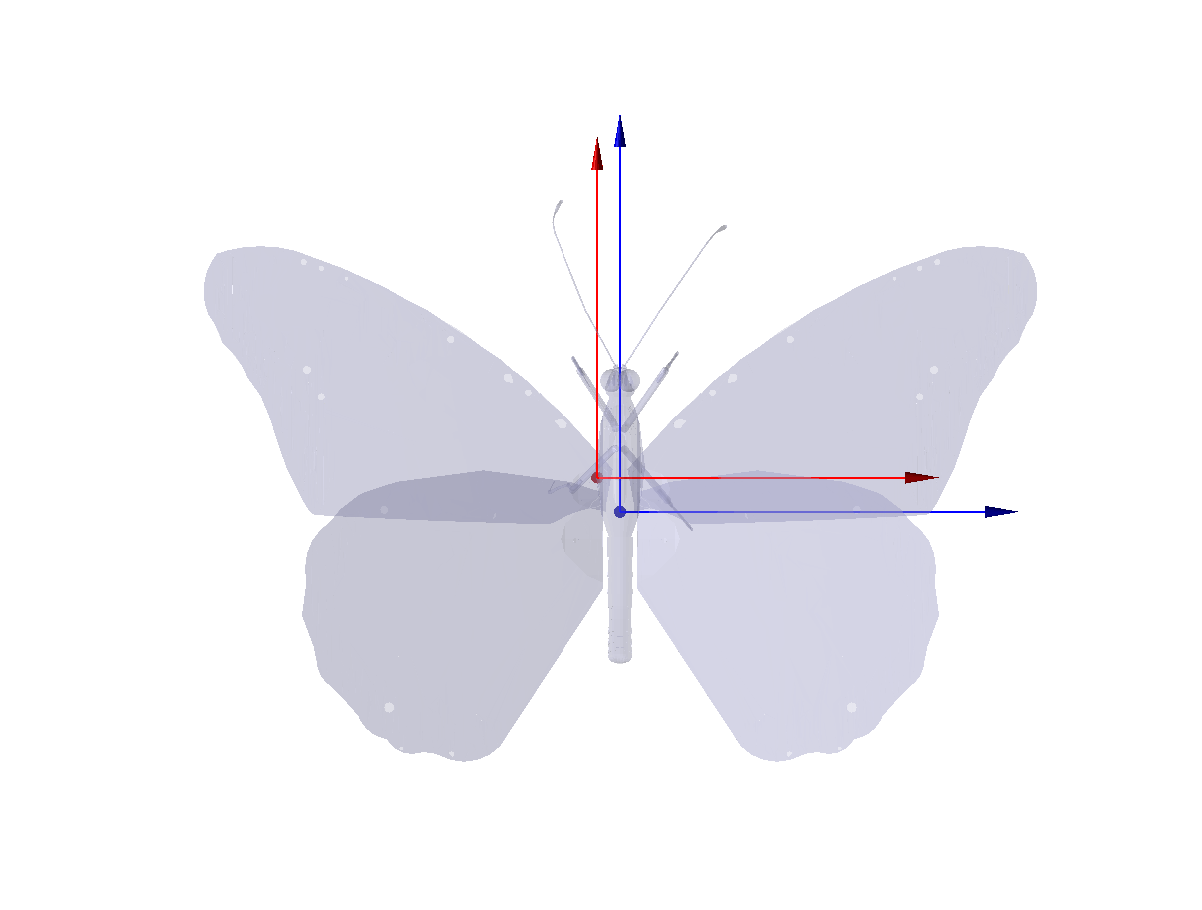
\includegraphics[trim={3cm 2cm 2cm 1cm},clip,width=0.3\textwidth]{monarch_FL}}
           \put(1.5,2.25){$\mathbf{b}_x$}
           \put(1.2,2.15){$\mathbf{l}_x$}
           \put(2.5,1.1){$\mathbf{l}_y$}
           \put(2.85,0.75){$\mathbf{b}_y$}
        \end{picture}
    \end{center}
    \caption{The body-fixed frame $\mathcal{F}_B=\{\mathbf{b}_x,\mathbf{b}_y,\mathbf{b}_z\}$ (blue), the left wing frame $\mathcal{F}_L=\{\mathbf{l}_x,\mathbf{l}_y,\mathbf{l}_z\}$ (red)}\label{fig:FL}
\end{figure}

Similar as the right wing, the motion of the left wing relative to the thorax is described by $Q_L\in\SO$, which is described by successive rotations as
\begin{align}
    Q_L(t) = \exp(\beta \hat e_2)\exp(-\phi_L(t) \hat e_1) \exp(\psi_L(t) \hat e_3) \exp(\theta_L(t) \hat e_2),\label{eqn:Q_L}
\end{align}
where the definition of the Euler-angles $(\phi_L,\theta_L,\psi_L)$ are consistent with those of the right wing.
The wing kinematics become symmetric when $(\phi_R,\theta_R,\psi_R)=(\phi_L,\theta_L,\psi_L)$. 
\nomenclature{$Q_L\in\SO$}{the attitude of the left wing,  the linear transformation of the representation of a vector from $\mathcal{F}_L$ to $\mathcal{F}_B$}
\nomenclature{$\Omega_L\in\Re^3$}{the angular velocity of the left wing relative to $\mathcal{F}_b$ resolved in $\mathcal{F}_L$}

The time-derivative of $Q_L$ is given by
\begin{align}
    \dot Q_L = Q_L \hat \Omega_L,
\end{align}
where $\Omega_L\in\Re^3$ is the angular velocity of the left wing relative to $\mathcal{F}_B$ resolved in $\mathcal{F}_L$.
Also, we have
\begin{align}
    \Omega_L & =
    \begin{bmatrix} 
        -\cos\psi_L\cos\theta_L & 0 & -\sin\theta_L \\
        \sin\psi_L & 1 & 0 \\
        -\cos\psi_L\sin\theta_L& 0& \cos\theta_L
    \end{bmatrix}
    \begin{bmatrix}
        \dot\phi_L \\ \dot\theta_L \\ \dot\psi_L
    \end{bmatrix}.
\end{align}

\subsection{Wing Kinematics}

We consider the wing kinematics model presented in~\cite{berman2007energy}.
Let $f\in\Re$ be the frequency of the flapping in $\mathrm{Hz}$.
Thus, the period of the flapping is $T=\frac{1}{f}$. 
\nomenclature{$f\in\Re$}{flapping frequency}
\nomenclature{$T\in\Re$}{flapping period}

The flapping angle is given by a smoothed triangular waveform,
\begin{align}
    \phi(t) & = \frac{\phi_m}{\sin^{-1} \phi_K}\sin^{-1}(\phi_K\cos(2\pi f t)) + \phi_0,\label{eqn:phi}
\end{align}
where $\phi_m\in\Re$ is the amplitude of flapping, and $\phi_0\in\Re$ is the offset. 
The parameter $0 < \phi_K \leq 1$ determines the shape of flapping waveform (sinusoidal when $\phi_K\rightarrow 0$; triangular when $\phi_K\rightarrow 1$).
The initial pitch angle is $\phi(0)=\phi_m+\phi_0$.
During $0\leq t \leq \frac{T}{2}$, the pitch angle decreases to $\phi(\frac{T}{2}) = -\phi_m+\phi_0$. 
Therefore, it represents upstroke when $0\leq t \leq \frac{T}{2}$, and it represents downstroke when $\frac{T}{2} \leq t \leq T$.

In~\cite{berman2007energy}, the inner term is given by $\sin(2\pi f t)$, instead of $\cos(2\pi f t)$ as in~\eqref{eqn:phi}. 
By following the convention of~\cite{bluman2017wing}, we use the cosine.
This is to ensure that in the subsequent expression of the pitch angle, the pitch angle reversal happens at the end of the downstroke or at the end of upstorke when there is no phase offset ($\theta_a=0$).

\nomenclature{$\phi_m\in[0,\frac{\pi}{2}]$}{flapping amplitude\nomrefeq}
\nomenclature{$\phi_o\in[\theta_m-\frac{\pi}{2},\frac{\pi}{2}-\theta_m]$}{flapping offset\nomrefeq}
\nomenclature{$\phi_K\in(0,1)$}{flapping waveform parameter\nomrefeq}

The pitch angle is given by a hyperbolic function,
\begin{align}
    \theta(t) = \frac{\theta_m}{\tanh \theta_C} \tanh( \theta_C \sin(2\pi f t + \theta_a)) +\theta_0,
\end{align}
where $\theta_m\in\Re$ is the amplitude of pitching, and $\theta_0\in\Re$ is the offset. 
The parameter $\theta_C\in(0,\infty)$ determines the waveform (sinusoidal when $\theta_C\rightarrow 0$; step function when $\theta_C\rightarrow \infty$).
The value of $\theta_C$ is related to the duration of the wing pitch reversal. 
The parameter $\theta_a\in(-\pi,\pi)$ describes the offset in phase (advance rotation for $\theta_a>0$; symmetric rotation for $\theta_a=0$; delayed rotation for $\theta_a<0$).
\nomenclature{$\theta_m\in[0,\frac{\pi}{2}]$}{pitching amplitude\nomrefeq}
\nomenclature{$\theta_o\in[\theta_m-\pi,\pi-\theta_m]$}{pitching offset\nomrefeq}
\nomenclature{$\theta_C\in(0,\infty)$}{pitching waveform parameter\nomrefeq}
\nomenclature{$\theta_a\in(-\pi,\pi)$}{pitching phase offset\nomrefeq}

Finally, the deviation angle is given by a sinusoidal oscillation,
\begin{align}
    \psi(t) = \psi_m \cos(2\pi \psi_N f t + \psi_a) + \psi_0,
\end{align}
where $\psi_m\in\Re$ is the amplitude of the deviation, and $\psi_0\in\Re$ is the offset. 
The parameter $\psi_N$ is either 1 or 2: $\psi_N=1$ corresponds to one oscillation per a flapping period, and $\psi_N=2$ corresponds to a figure-eight motion. 
The parameter $\psi_a\in(-\pi,\pi)$ describes the offset in phase. 
See Figure \ref{fig:wing_kinematics} for the trajectories of these angles for selected parameters. 
\nomenclature{$\psi_m\in\Re$}{deviation amplitude\nomrefeq}
\nomenclature{$\psi_o\in\Re$}{deviation offset\nomrefeq}
\nomenclature{$\psi_N\in\{1,2\}$}{deviation oscillation per a flapping\nomrefeq}
\nomenclature{$\psi_a\in(-\pi,\pi)$}{deviation phase offset\nomrefeq}

\begin{figure}
    \centerline{
        \includegraphics[width=0.7\textwidth]{wing_kinematics}
    }
    \caption{Wing kinematics when $\phi_m=50^\circ$, $\phi_0=10^\circ$, $\theta_m=45^\circ$, $\theta_0=0$, $\theta_a=0.3$, $\phi_m=10^\circ$, $\phi_0=\phi_a=0$}\label{fig:wing_kinematics} 
\end{figure}


\subsection{Abdomen}

Consider an abdomen that is assumed to be a rigid body attached to the thorax via a spherical joint. 
Let $\mathcal{F}_A=\{\mathbf{a}_x, \mathbf{a}_y, \mathbf{a}_z\}$ be the frame fixed to the abdomen.
Its origin is located at the mass center of the abdomen, and its orientation is identical to $\mathcal{F}_B$ when there is no rotation relative to the body. 
The vector from the origin of $\mathcal{F}_B$ to the joint connecting the thorax and the abdomen is $\mu_A\in\Re^3$. As it is resolved in $\mathcal{F}_B$ and the body is rigid, we have $\dot \mu_A=0$. 
\nomenclature{$\mathcal{F}_A$}{frame fixed to abdomen}
\nomenclature{$\mathbf{a}_x,\mathbf{a}_y,\mathbf{a}_z$}{basis vector of the abdomen-fixed frame}
\nomenclature{$\mu_A\in\Re^3$}{the fixed vector from the mass center of the body to the joint connecting the abdomen, resolved in $\mathcal{F}_B$}

The motion of the abdomen relative to the body is described by $Q_A\in\SO$, which is the linear transformation of the representation of a vector from $\mathcal{F}_A$ to $\mathcal{F}_B$. 
Its time-derivative is given by
\begin{align}
    \dot Q_A = Q_A \hat\Omega_A,
\end{align}
where $\Omega_A\in\Re^3$ is the angular velocity of the abdomen relative to the body, resolved in $\mathcal{F}_A$.

\nomenclature{$Q_A\in\SO$}{the attitude of the abdomen,  the linear transformation of the representation of a vector from $\mathcal{F}_A$ to $\mathcal{F}_B$}
\nomenclature{$\Omega_A\in\Re^3$}{the angular velocity of the abdomen relative to $\mathcal{F}_B$ resolved in $\mathcal{F}_R$}








\section{Quasi-Steady Aerodynamics}

The quasi-steady assumption implies that the aerodynamic force and moment generated by the flapping wing are equivalent to those for steady motion at the same instantaneous velocity and the angle of attack. 

\subsection{Wing Morphological Parameters}

\setlength{\unitlength}{0.1\columnwidth}
\begin{figure}[h]
    \begin{center}
        \footnotesize
        \begin{picture}(3,2.4)(0,0)
           \put(0,0){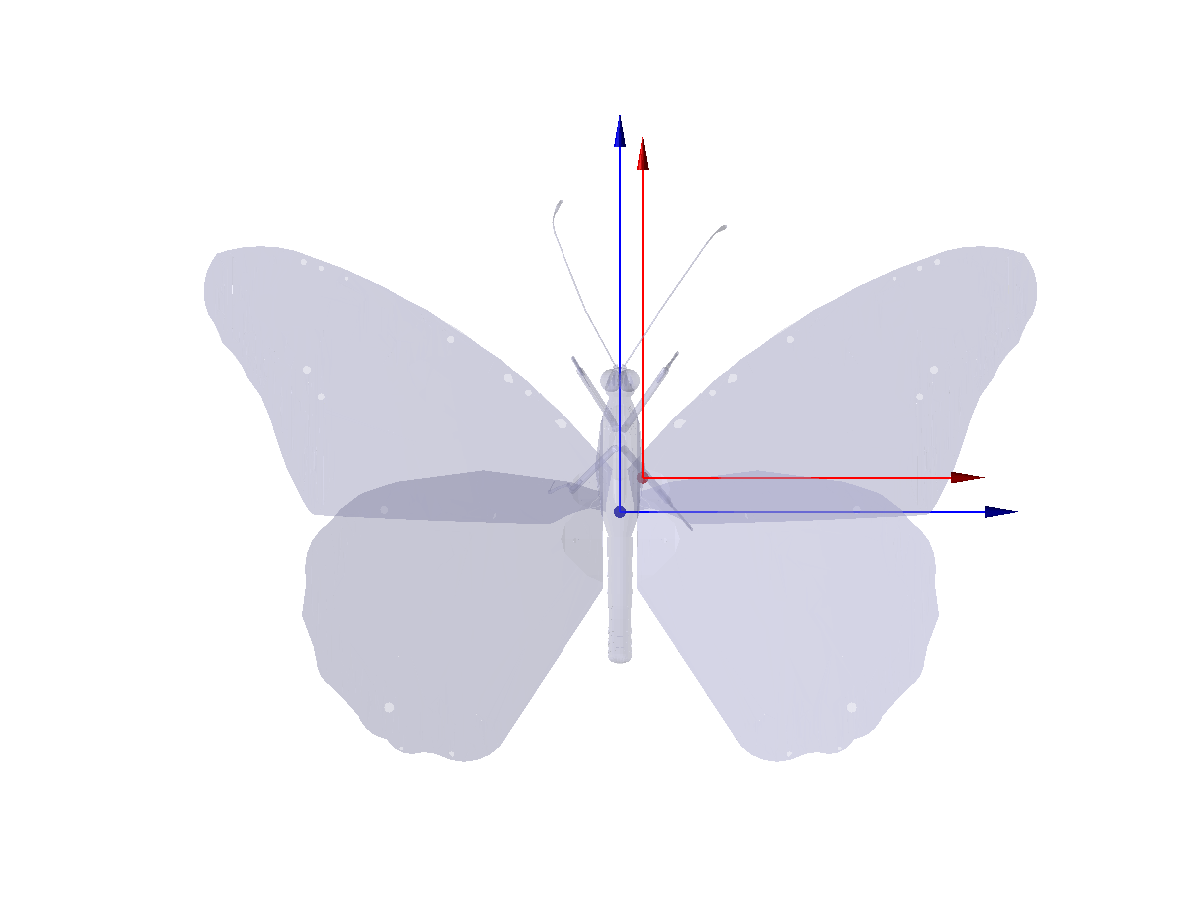
\includegraphics[trim={3cm 2cm 2cm 1cm},clip,width=0.3\textwidth]{monarch_FR}}
           \put(1.6,2.2){$\mathbf{r}_x$}
           \put(2.7,1.1){$\mathbf{r}_y$}
           \linethickness{0.2em}
           \put(2.1,1.57){\line(0,-1){1.50}}
           \put(2.15,0.7){$c(r)$}
           \put(2.05,-0.1){$dr$}
           \put(1.8,1.05){$r$}
        \end{picture}
    \end{center}
    \caption{Infinitesimal wing segment }\label{fig:wing_segment}
\end{figure}

We first present several morphological parameters of the wing as formulated in to~\cite{ellington1984aerodynamics}, after making a few changes in the notation.  
More specifically, in~\cite{ellington1984aerodynamics}, the symbol $\wedge$ is used to denote normalized variables. 
However, the same symbol is used for the hat map in \eqref{eqn:hat_map}.
Instead, we use the symbol $\tilde{\;\;}$ for the normalized variables to avoid conflict with~\eqref{eqn:hat_map}.
Also, the morphological parameters are defined for a single wing as the aerodynamic force of the left wing will be distinguished from the right wing for non-symmetric flapping. 

Let $dr$ be the infinitesimal wing segment located distanced at $r$ from the wing root. 
Let its chord be defined as $c(r)$. 
The wing segment is parallel to $\mathbf{r}_x$ and the distance is measured along $\mathbf{r}_y$.
Assume that the aerodynamic center of the segment is along $\mathbf{r}_y$, i.e., the resultant force generated by the wing segment is located along $\mathbf{r}_y$ with zero moment. 
Consequently, it is located at $re_2$ when resolved in $\mathcal{F}_R$.
\nomenclature{$c(r)\in\Re$}{the length of the chord at the distance $r$ from the wing root (see Figure~\ref{fig:wing_segment})}

The area of the right wing is given by
\begin{align}
    S = \int_0^{l} c(r) dr,
\end{align}
where $l>0$ is the wing span, i.e., the distance between the wing root and the wing tip measure along $\mathbf{r}_y$.
\nomenclature{$S\in\Re$}{the area of the right wing (In~\cite{ellington1984aerodynamics}, the symbol $S$ used for the total area of the left wing and the right wing)}%
\nomenclature{$l\in\Re$}{the span of the right wing, i.e., the length of the right wing from the wing root and the wing tip}%
The non-dimensional aspect ratio is
\begin{align}
    \AR = \frac{l^2}{S}.
\end{align}
\nomenclature{$\AR$}{the aspect ratio of the wing\nomrefeq}
The mean chord is the area divided by the span, i.e., $\bar c = \frac{S}{l}$, and the normalized wing chord is
\begin{align}
    \tilde c = \frac{c}{\bar c} = \frac{c l}{S}.
\end{align}
\nomenclature{$\bar c\in\Re$}{mean chord\nomrefeq}
\nomenclature{$\tilde c\in\Re$}{normalized chord\nomrefeq (this is equivalent to $\hat c$ in~\cite{ellington1984aerodynamics})}
Also, the non-dimensional radius is defined as
\begin{align}
    \tilde r = \frac{r}{l}.
\end{align}
\nomenclature{$\tilde r\in\Re$}{normalized radius\nomrefeq (this is equivalent to $\hat r$ in~\cite{ellington1984aerodynamics})}

The $k$-th moment of wing area is defined as
\begin{align}
    S_k = \int_0^{l} r^k c(r) dr = Sl^k \int_0^1 \tilde r^k \tilde c  d\tilde r,
\end{align}
satisfying $S_0=S$.
The non-dimensional radius of the $k$-th moment of wing area is defined as
\begin{align}
    \tilde r_k = \parenth{\frac{S_k}{Sl^k}}^{\frac{1}{k}} 
    = \parenth{\frac{1}{Sl^k} \int_0^{l} r^k c(r) dr}^{\frac{1}{k}} 
    = \parenth{\int_0^1 \tilde r^k \tilde c d\tilde r}^{\frac{1}{k}}, \label{eqn:tilde_r_k}
\end{align}
such that $S_k = (\tilde r_k l)^k S$, i.e., if all of the wing area is located at a distance $\tilde r_k l$, the $k$-th moment of area is equal to $S_k$.
\nomenclature{${S_k \in\Re}$}{the $k$-th moment of wing area}
\nomenclature{${\tilde r_k \in\Re}$}{non-dimensional radius of the $k$-th moment of wing area (this is equivalent to $\hat r_k(S)$, or (7) of ~\cite{ellington1984aerodynamics})}

Next, when a wing is accelerated, it causes the motion of the surrounding air.
The inertia of the wing is increased by the mass of air that is accelerated, and therefore there is an increase in the wing mass. 
The normalized virtual mass is defined as
\begin{align}
    \tilde v = \int_0^1 \tilde c^2 d\tilde r.
\end{align}
\nomenclature{${\tilde v \in\Re}$}{non-dimensional virtual mass of the wing (this is equivalent to $\hat v$, or (14) of ~\cite{ellington1984aerodynamics})}
%
And the corresponding normalized radius of the $k$-th moment of virtual mass is 
\begin{align}
    \tilde r_k (v) = \parenth{ \frac{1}{\tilde v} \int_0^1 \tilde c^2 \tilde r^k d\tilde r }^{\frac{1}{k}}.
\end{align}
\nomenclature{${\tilde r_k(v) \in\Re}$}{non-dimensional radius of the $k$-th moment of wing volume (this is equivalent to $\hat r_k(v)$, or (16) of ~\cite{ellington1984aerodynamics})}

Later, we need to compute the following quantity:
\begin{align}
    \int_0^l r c^2(r) dr & = l^2 \bar c^2 \int_0^1 \tilde r \tilde c^2 d\tilde r = l^2 \bar c^2 \tilde v \tilde r_1(v),\label{eqn:int_rc2dr} \\
    \int_0^l r^2 c^2(r) dr & = l^3 \bar c^2 \int_0^1 \tilde r^2 \tilde c^2 d\tilde r = l^2 \bar c^2 \tilde v \tilde r_2^2(v).\label{eqn:int_r2c2dr} 
\end{align}

\subsection{Blade-Element Theory}

\paragraph{Angle of Attack of Right Wing}

When resolved in the inertial frame, the root of the right wing is located at $x+R\mu_R$. 
Thus, the aerodynamic center of the chord at the distance $r$ from the wing root is
\[
    x+R\mu_R + RQ_R r e_2.
\]
Therefore, its velocity in $\mathcal{F}_I$ is 
\[
    \dot x+ R\hat\Omega \mu_R + R \hat\Omega Q_R re_2 + R Q_R \hat \Omega_R r e_2,   
\]
which is transformed to $\mathcal{F}_R$ by left-multiplying $Q_R^T R^T$ as
\begin{align*}
    Q_R^T R^T \dot x & +  Q_R^T \hat\Omega \mu_R +  Q_R^T \hat\Omega Q_R re_2 +  \hat \Omega_R r e_2\\
              & = Q_R^T( R^T \dot x + \Omega\times \mu_R ) + r  (Q_R\Omega + \Omega_R )\times e_2,
\end{align*}
where the first term corresponds to the velocity of the wing root and the second term corresponds to the velocity of the aerodynamic center relative to the wing root. 
Both are resolved in $\mathcal{F}_R$. 

Assume that there is a uniform wind with the velocity $v_{\mathrm{wind}}\in\Re^3$ resolved in $\mathcal{F}_I$. 
The velocity of the aerodynamic center of $c(r)$ relative to the wind is given by
\begin{align*}
    Q_R^T( R^T (\dot x-v_{\mathrm{wind}}) + \Omega\times \mu_R ) + r  (Q_R\Omega + \Omega_R )\times e_2,
\end{align*}
According to the \textit{blade-element theory}~\cite{ellington1984aerodynamics}, the aerodynamic force generated by the infinitesimal chord is independent of the span-wise velocity component, i.e., the component of the above expression along $\mathbf{r}_y$ is irrelevant. 
Therefore, we project the above velocity to the $\mathbf{r}_x$--$\mathbf{r}_z$ plane as follows.
\begin{align}
    U_R(r) = (I_{3\times 3}- e_2 e_2^T) Q_R^T( R^T (\dot x-v_{\mathrm{wind}}) + \Omega\times \mu_R ) + r  (Q_R\Omega + \Omega_R )\times e_2.\label{eqn:Ur}
\end{align}
where $I_{3\times 3} - e_2e_2^T= \mathrm{diag}[1,0,1]\in\Re^{3\times 3}$ corresponds to the projection operator. 
The second term is not affected by the projection as it is already normal to $e_2$.
\nomenclature{$U(r)\in\Re^3$}{the velocity of the aerodynamic center of the chord $c(r)$ relative to the ambient wind, resolved in the wing fixed frame; this is projected to the $\mathbf{r}_x$--$\mathbf{r}_z$ plane so that the second component is always zero\nomrefeq}

The angle of attack $\alpha_R(r)$ is the angle between the chord line $\pm e_1$ and the above velocity $U_R(r)$. 
Assuming that the chord is a thin blade, when the angle is greater than $\frac{\pi}{2}$, we flip the leading edge and the trailing edge of the chord.
This ensures that $\alpha_R(r)\in[0,\frac{\pi}{2}]$ always. 
More explicitly, 
\begin{align}
    \alpha_R (r) & = 
    \cos^{-1} ( \frac{|e_1^T U_R(r)|}{\|U_R(r)\|} ).\label{eqn:alpha}
\end{align}
The above expression has a singularity when $U(r)=0$. 
But, the value of $\alpha(r)$ does not matter when $U(r)=0$, as the resulting aerodynamic force and moment will vanish.
Or equivalently, it can be written as
\begin{align}
    \alpha_R (r) & = 
    \sin^{-1} ( \frac{|e_3^T U_R(r)|}{\|U_R(r)\|} ).\label{eqn:alpha_3}
\end{align}
\nomenclature{$\alpha\in[0,\frac{\pi}{2}]$}{angle of attack}

\paragraph{Angle of Attack of Left Wing}

For the left wing, \eqref{eqn:Ur} is changed into
\begin{align}
    U_L(r) = (I_{3\times 3}- e_2 e_2^T) Q_L^T( R^T (\dot x-v_{\mathrm{wind}}) + \Omega\times \mu_L ) - r  (Q_L\Omega + \Omega_L )\times e_2.\label{eqn:Ur_R}
\end{align}
The angle of attack is given by
\begin{align}
    \alpha_L (r) & = 
    \cos^{-1} ( \frac{|e_1^T U_L(r)|}{\|U_L(r)\|} ) = 
    \sin^{-1} ( \frac{|e_3^T U_L(r)|}{\|U_L(r)\|} ).\label{eqn:alpha_3_L}
\end{align}

\subsection{Translational Forces}

\paragraph{Right Wing}

Here we find the expression of the lift and the drag. 
The magnitude of the lift generated by the infinitesimal wing segment $c(r)$ is
\[
    \frac{1}{2}\rho \|U_R(r)\|^2 C_L(\alpha_R(r)) c(r) dr,
\]
where $\rho\in\Re$ is the atmospheric density, and $C_L\in\Re$ is the lift coefficient given as a function of the angle of attack. 
\nomenclature{$\rho\in\Re$}{atmospheric density}
\nomenclature{$C_L\in\Re$}{lift coefficient}

The direction of the lift is normal to both of the velocity $U_R(r)$ and the wing span-wise direction $e_2$. 
As such, the direction of the lift is along $\pm e_2\times U_R(r)$ in $\mathcal{F}_R$. 
The ambiguity of the sign can be resolved by the fact that when the $\mathbf{r}_x$--$\mathbf{r}_z$ plane is divided by the chord line $\mathbf{r}_x$, the velocity vector $U(r)$ and the lift vector occupy the opposite side with each other. 
\begin{figure}
    \centerline{
        \footnotesize
        \subfigure[Case 1]{
            \begin{picture}(2.5,2.5)(0,0)
                \put(1.25,1.25){\vector(-2,-1){1}}
                \put(1.25,1.25){\vector(-1,2){0.5}}
                \put(0.2,0.5){$U_R(r)$}
                \put(0.0,2.0){\shortstack[c]{$dL_R\parallel$\\$e_2\times U_R(r)$}}
                \put(1.25,1.25){\line(1,0){1}}
                \put(1.55,1.3){chord}
                \linethickness{0.1em}
                \put(1.25,1.25){\vector(-1,0){1}}
                \put(1.25,1.25){\vector(0,-1){1}}
                \put(0.15,1.35){$\mathbf{r}_x$}
                \put(1.3,0.2){$\mathbf{r}_z$}
                \put(0.8,1.12){$\alpha$}
            \end{picture}
        }
        \subfigure[Case 2]{
            \begin{picture}(2.5,2.5)(0,0)
                \put(1.25,1.25){\vector(2,-1){1}}
                \put(1.25,1.25){\vector(1,2){0.5}}
                \put(2.0,0.6){$U_R(r)$}
                \put(0.8,2.0){\shortstack[c]{$dL_R\parallel$\\$-e_2\times U_R(r)$}}
                \put(1.25,1.25){\line(1,0){1}}
                \put(1.55,1.12){$\alpha$}
                \put(1.55,1.3){chord}
                \linethickness{0.1em}
                \put(1.25,1.25){\vector(-1,0){1}}
                \put(1.25,1.25){\vector(0,-1){1}}
                \put(0.15,1.35){$\mathbf{r}_x$}
                \put(1.3,0.2){$\mathbf{r}_z$}
            \end{picture}
        }
        \subfigure[Case 3]{
            \begin{picture}(2.5,2.5)(0,0)
                \put(1.25,1.25){\vector(-2,1){1}}
                \put(1.25,1.25){\vector(-1,-2){0.5}}
                \put(0.1,1.9){$U_R(r)$}
                \put(0.2,0.5){\shortstack[c]{$dL_R\parallel$\\$-e_2\times U_R(r)$}}
                \put(0.8,1.3){$\alpha$}
                \put(1.25,1.25){\line(1,0){1}}
                \put(1.55,1.3){chord}
                \linethickness{0.1em}
                \put(1.25,1.25){\vector(-1,0){1}}
                \put(1.25,1.25){\vector(0,-1){1}}
                \put(0.15,1.35){$\mathbf{r}_x$}
                \put(1.3,0.2){$\mathbf{r}_z$}
            \end{picture}
        }
        \subfigure[Case 4]{
            \begin{picture}(2.5,2.5)(0,0)
                \put(1.25,1.25){\vector(2,1){1}}
                \put(1.25,1.25){\vector(1,-2){0.5}}
                \put(1.9,1.85){$U_R(r)$}
                \put(1.6,0.1){\shortstack[c]{$dL_R\parallel$\\$e_2\times U_R(r)$}}
                \put(1.25,1.25){\line(1,0){1}}
                \put(1.55,1.3){$\alpha$}
                \put(1.55,1.10){chord}
                \linethickness{0.1em}
                \put(1.25,1.25){\vector(-1,0){1}}
                \put(1.25,1.25){\vector(0,-1){1}}
                \put(0.15,1.35){$\mathbf{r}_x$}
                \put(1.3,0.2){$\mathbf{r}_z$}
            \end{picture}
        }
    }
    \caption{Direction of the velocity and the lift in the $\mathbf{r}_x$--$\mathbf{r}_z$ plane of the right wing}\label{fig:lift_direction}
\end{figure}

More specifically, consider the four cases illustrated in Figure~\ref{fig:lift_direction}.
These show that the direction of lift is $e_2\times U_R(r)$ when $e_1^T U_R(r)$ and $e_3^TU_R(r)$ have the same sign (Case 1 and Case 4), and it is $-e_2\times U_R(r)$ when they have the opposite sign (Case 2 and Case 3).
Therefore, the infinitesimal lift vector resolved in $\mathcal{F}_R$ is given by
\begin{align}
    dL_R(r) & = \frac{1}{2}\rho U_R^2(r) C_L(\alpha(r)) c(r) \mathrm{sgn} (e_1^T U_R(r) e_3^T U_R(r)) \frac{e_2\times U_R(r)}{\|e_2\times U(r)\|} dr \nonumber \\
            & = \frac{1}{2}\rho  C_L(\alpha(r)) c(r) \mathrm{sgn} (e_1^T U_R(r) e_3^T U_R(r)) (e_2\times U_R(r))\|U_R(r)\|  dr,\label{eqn:dLR}
\end{align}
where the second equality is obtained by $\|U_R(r)\|=\|e_2\times U_R(r)\|$.

The total lift of the right wing is obtained by integrating above span-wise for $r\in[0,l]$.
\begin{align}
    L_R = \int_{0}^{l} dL_R(r),
\end{align}
which is resolved in $\mathcal{F}_R$. 
\nomenclature{$L_R\in\Re^3$}{the lift vector of the right wing resolved in $\mathcal{F}_R$}

Next, the drag is always opposite to $U_R(r)$. 
Similar with the above expressions, 
\begin{align}
    dD_R(r) = - \frac{1}{2}\rho  C_D(\alpha(r)) c(r) \|U_R(r)\|U_R(r) dr.
\end{align}
The total drag is obtained by integrating above span-wise for $r\in[0,l]$ as
\begin{align}
    D_R = \int_{0}^{l} dD_R (r),
\end{align}
which is resolved in $\mathcal{F}_R$. 
\nomenclature{$D_R\in\Re^3$}{the drag vector of the right wing resolved in $\mathcal{F}_R$}

The lift and the drag also generate the moment about the wing root. 
When resolved in $\mathcal{F}_R$, it is given by
\begin{align}
    M_R = \int_{0}^l r e_2 \times (dL_R + dD_R).
\end{align}
\nomenclature{$M_R\in\Re^3$}{moment about the wing root caused by the lift and the drag of the right wing, resolved in $\mathcal{F}_R$}

\paragraph{Left Wing}

Similarly, the infinitesimal lift vector of the left wing resolved in $\mathcal{F}_L$ is given by
\begin{align}
    dL_L(r)  & = \frac{1}{2}\rho  C_L(\alpha(r)) c(r) \mathrm{sgn} (e_1^T U_L(r) e_3^T U_L(r)) (e_2\times U_L(r))\|U_L(r)\|  dr,\label{eqn:dLL}
\end{align}
which is integrated to obtain
\begin{align}
    L_L & = \int_0^l dL_L(r).
\end{align}
\nomenclature{$L_L\in\Re^3$}{the lift vector of the left wing resolved in $\mathcal{F}_L$}
Also, the infinitesimal drag of the left wing is
\begin{align}
    dD_L(r) = - \frac{1}{2}\rho  C_D(\alpha(r)) c(r) \|U_L(r)\|U_L(r) dr,
\end{align}
and
\begin{align}
    D_L = \int_{0}^{l} dD_L (r),
\end{align}
which is resolved in $\mathcal{F}_R$. 
\nomenclature{$D_L\in\Re^3$}{the drag vector of the left wing resolved in $\mathcal{F}_L$}

The lift and the drag also generate the moment about the wing root as
\begin{align}
    M_L = \int_{0}^l - r e_2 \times (dL_L + dD_L).
\end{align}
\nomenclature{$M_L\in\Re^3$}{moment about the wing root caused by the lift and the drag of the left wing, resolved in $\mathcal{F}_L$}

\subsection{Translational Forces for Small Body Velocities}

This above expression requires span-wise integration at every instance to compute the lift and the drag. 
Here we present an explicit expression for a special case when the linear velocity and the angular velocity of the body and the wind velocity are small. i.e., $\|\dot x\|, \|\Omega\|, \|v_{\mathrm{wind}}\| \ll 1$.  

\paragraph{Right Wing}

Under these assumptions, the first part of \eqref{eqn:Ur} vanishes so that the velocity reduces to 
\begin{align*}
    U_R(r) & = r \Omega_R \times e_2,
%    \\
         %& = r  
    %\begin{bmatrix} 
        %\cos\psi_R\cos\theta_R & 0 & \sin\theta_R \\
        %\sin\psi_R & 1 & 0 \\
        %\cos\psi_R\sin\theta_R& 0& -\cos\theta_R
    %\end{bmatrix}
    %\begin{bmatrix}
        %\dot\phi_R \\ \dot\theta_R \\ \dot\psi_R
    %\end{bmatrix} \times e_2 \\
         %& = r  
    %\begin{bmatrix} 
        %-\cos\psi_R\sin\theta_R&  \cos\theta_R\\
        %0 & 0 \\
        %\cos\psi_R\cos\theta_R & \sin\theta_R \\
    %\end{bmatrix}
    %\begin{bmatrix}
        %\dot\phi_R \\  \dot\psi_R
%    \end{bmatrix}.
\end{align*}
which is directly proportional to $r$. 
In~\eqref{eqn:alpha}, this eliminates the dependency of $\alpha$  on $r$ as follows.
\begin{align*}
    \alpha & = \cos^{-1} (\frac{ |e_1^T (\Omega_R \times e_2)|}{\|\Omega_R\times e_2\|}) = \cos^{-1} (\frac{ |e_3^T \Omega_R |}{\|\Omega_R \times e_2\|} ).
\end{align*}
In other words, the angle of attack is identical for all the infinitesimal chord in the right wing. 
Also, from \eqref{eqn:dLR},
\begin{align}
    dL_R(r) & = \frac{1}{2}\rho  C_L(\alpha) c(r) \mathrm{sgn} (e_1^T (\Omega_R\times e_2) e_3^T (\Omega_R\times e_2) ) (e_2\times (\Omega_R\times e_2))\|\Omega_R\times e_2\| r^2 dr\nonumber \\
            & = \frac{1}{2}\rho  C_L(\alpha) c(r) \mathrm{sgn} (-e_3^T \Omega_R e_1^T \Omega_R ) (e_2\times (\Omega_R\times e_2))\|\Omega_R\times e_2\| r^2 dr\nonumber \\
            & = \frac{1}{2}\rho  C_L(\alpha) c(r) \mathrm{sgn} (e_3^T \Omega_R e_1^T \Omega_R ) \hat e_2^2 \Omega_R \|\Omega_R\times e_2\|  r^2 dr\nonumber.
\end{align}
Consequently, the lift of the right wing is given by
\begin{align*}
    L_R & = \frac{1}{2}\rho  C_L(\alpha) \mathrm{sgn} (e_3^T \Omega_R e_1^T \Omega_R ) \hat e_2^2 \Omega_R \|\Omega_R\times e_2\| \int_{0}^{l} c(r)  r^2 dr,
\end{align*}
and using \eqref{eqn:tilde_r_k}
\begin{align*}
    L_R & = \frac{1}{2}\rho  C_L(\alpha) \mathrm{sgn} (e_3^T \Omega_R e_1^T \Omega_R ) \hat e_2^2 \Omega_R \|\Omega_R\times e_2\| l^2 \tilde r_2^2 S,
\end{align*}
which can be evaluated by $\Omega_R$ without integration over the wing span. 

Or, equivalently, define the velocity of the chord at $r=\tilde r_2 l$ as 
\begin{align}
    U_R = U_R(\tilde r_2 l) = \tilde r_2 l \Omega_R \times e_2. \label{eqn:U_R}
\end{align}
\nomenclature{$U_R\in\Re^3$}{the velocity of the chord at $r=\tilde r_2 l$ of the right wing\nomrefeq}
The angle of attack can be rewritten as
\begin{align}
    \alpha_R & = \cos^{-1} (\frac{ |e_1^T U_R|}{\|U_R\|}) = \sin^{-1} (\frac{ |e_3^T U_R|}{\|U_R\|}). \label{eqn:alpha_R}
\end{align}
Thus, the lift of the right wing resolved in $\mathcal{F}_R$ is given by
\begin{align}
    L_R & = \frac{1}{2}\rho  C_L(\alpha) \mathrm{sgn} (e_1^T U_R e_3^T U_R ) \hat e_2 U_R \|U_R\| S,
\end{align}
Similarly, the drag is given by
\begin{align}
    D_R = - \frac{1}{2}\rho  C_D(\alpha)  \|U_R \| U_R  S.
\end{align}
In short, for the special case of small body velocities, the lift and the drag vector of the right wing resolved in $\mathcal{F}_R$ are given by \eqref{eqn:U_R}--\eqref{eqn:alpha_R}.

Define $r_{cp}\in\Re$ such that the above moment is equivalent to the lift and the drag acting on $r_{cp}e_2$, i.e., 
\[
    r_{cp}e_2 \times \int (dL_R + dD_R) = \int re_2 \times (dL_R + dD_R).
\]
For the special case discussed above, one can show
\begin{align}
    r_{cp} & = \dfrac{ \int_{0}^l r^3 c(r) dr}{\int_0^l r^2 c(r) dr} = \frac{S_3}{S_2} = \frac{Sl^3 \tilde r_3^3}{S l^2 \tilde r_2^2} = \frac{\tilde r_3^3}{\tilde r_2^2} l.
\end{align}
\nomenclature{$r_{cp}\in\Re$}{distance from the wing root to the aerodynamic center of the lift and the drag\nomrefeq}
Therefore, the span-wise location of the center of pressure of the right wing is given by $r_{cp}e_2$, and the resulting moment about the wing root is
\begin{align}
    M_R = r_{cp} e_2 \times (L_R + D_R),
\end{align}
which is resolved in $\mathcal{F}_R$.

\paragraph{Left Wing}

For the left wing, define the velocity at the chord $r =\tilde r_2l$ be
\begin{align}
    U_L = U_L(\tilde r_2 l) = -\tilde r_2 \Omega_2 \times e_2.
\end{align}
\nomenclature{$U_L\in\Re^3$}{the velocity of the chord at $r=\tilde r_2 l$ of the left wing\nomrefeq}
The angle of attack is given by
\begin{align}
    \alpha_L & = \cos^{-1} (\frac{ |e_1^T U_L|}{\|U_L\|}) = \sin^{-1} (\frac{ |e_3^T U_L|}{\|U_L\|}). \label{eqn:alpha_L}
\end{align}
The translational force and the moment for the left wing are 
\begin{align}
    L_L & = \frac{1}{2}\rho  C_L(\alpha) \mathrm{sgn} (e_1^T U_L e_3^T U_L ) \hat e_2 U_L \|U_L\| S,\\
    D_L & = - \frac{1}{2}\rho  C_D(\alpha)  \|U_L \| U_L  S,\\
    M_L & = - r_{cp} e_2 \times (L_L + D_L),\label{eqn:M_L}
\end{align}
which are resolved in $\mathcal{F}_L$. 
All of these expressions are consistent with the right wing, except the negative sign in \eqref{eqn:M_L}. 

\subsection{Rotational Force}


The wing's own rotation may cause additional circulation about the chord that generate a normal force. 
This is referred to as a rotational force~\cite{sane2002aerodynamic}.
The expression of the rotational force of the right wing is identical to that of the left wing, except the flipped sign in the corresponding moment. 
As such, in this section, we do not distinguish the right wing from the left wing with the subscript $R$. 

According to~\cite{sane2002aerodynamic}, the magnitude of the rotational lift for the infinitesimal wing segment is given by
\begin{align}
    \rho \|U(r)\| C_\rot |\dot\alpha(r)|  c^2(r) dr,\label{eqn:F_rot_mag}
\end{align}
where the last part $C_\rot |\dot\alpha(R)| c^2$ corresponds to the rotational circulation.
From \eqref{eqn:alpha_R}, the time-derivative of the angle of attack multiplied by $\|U\|$ is given by
\begin{align}
    \|U\| \dot \alpha & = \frac{1}{\sin\alpha} \braces{ \cos\alpha \frac{U^T \dot U}{\|U\|} - {\mathrm{sgn}(e_1^T U)(e_1^T \dot U)}} \nonumber\\
    & = \frac{1}{\cos\alpha} \braces{ -\sin\alpha \frac{U^T \dot U}{\|U\|} + {\mathrm{sgn}(e_3^T U)(e_3^T \dot U)}}.
\end{align}
To avoid singularity caused by $\alpha$, the first expression is used when $\alpha$ is close to $\frac{\pi}{2}$, and the second expression is used when $\alpha$ is close to $0$. 
Also, to mitigate the singularity caused by $\|U\|\ll 1$, we evaluate $\|U\|\dot\alpha$ in the numerical implementation, instead of computing $\dot\alpha$ directly.  

Next, we find the direction of the rotational lift. 
It is shown that the rotational lift is always perpendicular to the chord line, and consequently it is $\pm e_3$ in $\mathcal{F}_R$. 
Consider the four cases of $\alpha >0$ illustrated in Figure \ref{fig:lift_direction}.
For the first two cases of $e_3^T U >0$, $\dot\alpha >0$ generates the rotational lift along $-e_3$, and for the last two cases of $e_3^T U(r) <0$,  $\dot\alpha>0$ generates the rotational lift along $e_3$. 
Therefore, when $\alpha >0$, the direction of the rotational lift is $-\mathrm{sgn}(e_3^T U) \mathrm{sgn}(\dot\alpha) e_3$.

\begin{figure}[h]
    \centerline{
        \footnotesize
        \subfigure[Case 1]{
            \begin{picture}(2.5,2.5)(0,0)
                \put(1.25,1.25){\vector(-2,0){1}}
                \put(1.25,1.25){\vector(0,1){1}}
                \put(0.25,1.20){\vector(0,-1){0.3}}
                \put(0.0,1.35){$U(r)$}
                \put(0.0,0.65){$e_3^T\dot U(r)>0$}
                \put(1.3,2.2){$F_\rot$}
                \put(1.25,1.25){\line(1,0){1}}
                \put(1.55,1.3){chord}
                \linethickness{0.1em}
                \put(1.25,1.25){\vector(-1,0){0.6}}
                \put(1.25,1.25){\vector(0,-1){0.6}}
                \put(0.75,1.35){$\mathbf{r}_x$}
                \put(1.3,0.6){$\mathbf{r}_z$}
            \end{picture}
        }
        \subfigure[Case 2]{
            \begin{picture}(2.5,2.5)(0,0)
                \put(1.25,1.25){\vector(-2,0){1}}
                \put(1.25,1.25){\vector(0,-1){1}}
                \put(0.25,1.3){\vector(0,1){0.3}}
                \put(0.0,1.05){$U(r)$}
                \put(0.0,1.7){$e_3^T\dot U(r)<0$}
                \put(1.3,0.2){$F_\rot$}
                \put(1.25,1.25){\line(1,0){1}}
                \put(1.55,1.3){chord}
                \linethickness{0.1em}
                \put(1.25,1.25){\vector(-1,0){0.6}}
                \put(1.25,1.25){\vector(0,-1){0.6}}
                \put(0.75,1.35){$\mathbf{r}_x$}
                \put(1.3,0.6){$\mathbf{r}_z$}
            \end{picture}
        }
        \subfigure[Case 3]{
            \begin{picture}(2.5,2.5)(0,0)
                \put(1.25,1.25){\vector(2,0){1}}
                \put(1.25,1.25){\vector(0,1){1}}
                \put(2.25,1.20){\vector(0,-1){0.3}}
                \put(2.0,1.35){$U(r)$}
                \put(1.8,0.65){$e_3^T\dot U(r)>0$}
                \put(1.3,2.2){$F_\rot$}
                \put(1.25,1.25){\line(-1,0){1}}
                \put(0.3,1.0){chord}
                \linethickness{0.1em}
                \put(1.25,1.25){\vector(-1,0){0.6}}
                \put(1.25,1.25){\vector(0,-1){0.6}}
                \put(0.75,1.35){$\mathbf{r}_x$}
                \put(1.3,0.6){$\mathbf{r}_z$}
            \end{picture}
        }
        \subfigure[Case 4]{
            \begin{picture}(2.5,2.5)(0,0)
                \put(1.25,1.25){\vector(2,0){1}}
                \put(1.25,1.25){\vector(0,-1){1}}
                \put(2.25,1.3){\vector(0,1){0.3}}
                \put(2.0,1.05){$U(r)$}
                \put(1.8,1.7){$e_3^T\dot U(r)<0$}
                \put(1.3,0.2){$F_\rot$}
                \put(1.25,1.25){\line(-1,0){1}}
                \put(0.3,1.0){chord}
                \linethickness{0.1em}
                \put(1.25,1.25){\vector(-1,0){0.6}}
                \put(1.25,1.25){\vector(0,-1){0.6}}
                \put(0.75,1.35){$\mathbf{r}_x$}
                \put(1.3,0.6){$\mathbf{r}_z$}
            \end{picture}
        }
    }
    \caption{Direction of the rotational lift when $\alpha=0$}\label{fig:lift_rot}
\end{figure}

For the case of $\alpha=0$, the direction of the rotational lift is illustrated in Figure \ref{fig:lift_rot}, where the rotational lift is always opposite to $e_3^T \dot U$.
Therefore, its direction is given by $-\mathrm{sgn}(e_3^T \dot U) e_3$. 

These two cases for the direction can be combined into
\begin{equation}
    \mathrm{sig}_\rot (r) e_3, 
\end{equation}
where
\begin{equation}
    \mathrm{sig}_\rot = \mathrm{sgn}(\alpha(r))\{-\mathrm{sgn}(e_3^T U(r) )\mathrm{sgn}(\dot \alpha(r)) \} + (1-\mathrm{sgn}(\alpha(r)))\{-\mathrm{sgn}(e_3^T \dot U(r)) \},
\end{equation}
which takes the value of $\pm 1$. 
Thus, the rotational lift vector is the product of the above direction and the magnitude \eqref{eqn:F_rot_mag}. 
\begin{align}
d F_\rot & = \rho \|U(r)\| C_\rot |\dot\alpha(r)| \mathrm{sgn}_\rot (r) e_3  c^2(r) dr,
\end{align}
which is integrated to obtain the rotational force
\begin{align}
    F_\rot = \int_0^{l} dF_\rot.
\end{align}
\nomenclature{$F_\rot\in\Re^3$}{rotational force resolved in the wing fixed frame}

For the right wing, the above rotational force generate the moment about the wing root as follows.
\[
    M_{\rot_R} = \int_0^l re_2 \times d F_\rot,
\]
which is resolved in $\mathcal{F}_R$. 
For the left wing, the chord is located at $-r e_2$ in $\mathcal{F}_L$, and consequently
\[
    M_{\rot_L} = -\int_0^l re_2 \times d F_\rot.
\]
\nomenclature{$M_\rot\in\Re^3$}{moment about the wing root due to the rotational force, resolved in the wing fixed frame}

\subsection{Rotational Force for Small Body Velocities}

\paragraph{Right Wing}

Under the assumption of small body velocities, we present an expression for the rotational force that does not require a span-wise integration. 
As discussed above, when $\|\dot x\|,\|\Omega\|, \|v_{\mathrm{wind}}\| \ll 1$, $U_R(r)$ reduces to
\[
    U_R(r) = r \Omega_R \times e_2,
\]
so that $\alpha,\dot\alpha$ remains fixed span-wise. 
Thus,
\begin{align*}
    F_{\rot_R} & = \rho C_\rot  \|\Omega_R \times e_2 \| |\dot\alpha(t)|\; \mathrm{sgn}_\rot(t)  e_3 \int_0^l r c^2(r) dr,
\end{align*}
Substituting \eqref{eqn:int_rc2dr},
\begin{align*}
    F_{\rot_R} & = \rho C_\rot  \|\Omega_R \times e_2 \| |\dot\alpha(t)|\; \mathrm{sgn}_\rot(t)  e_3 l^2 \bar c^2 \tilde v \tilde r_1(v).
\end{align*}
Substituting \eqref{eqn:U_R}, we obtain the rotational force in terms of $U_R$ as 
\begin{align}
    F_{\rot_R} & = \rho C_\rot  \|U_R \| |\dot\alpha(t)|\; \mathrm{sgn}_\rot(t)  e_3 l \bar c^2 \frac{\tilde v \tilde r_1(v)}{\tilde r_2}. \label{eqn:F_rot}
\end{align}

Define $r_\rot\in\Re$ such that the moment about the wing root generated by the rotational force is written as
\begin{equation}
    M_{\rot_R} = r_\rot e_2 \times F_{\rot_R}.
\end{equation}
Using \eqref{eqn:int_rc2dr} and \eqref{eqn:int_r2c2dr}, one can show
\begin{align}
    r_\rot & = \frac{\int_0^l r^2 c^2(r) dr}{\int_0^l r c^2(r) dr} = \frac{l\tilde r_2^2(v)}{\tilde r_1(v)}.
\end{align}

\paragraph{Left Wing}

For the left wing,
\begin{align}
    F_{\rot_L} & = \rho C_\rot  \|U_L \| |\dot\alpha(t)|\; \mathrm{sgn}_\rot(t)  e_3 l \bar c^2 \frac{\tilde v \tilde r_1(v)}{\tilde r_2}, \label{eqn:F_rot_L}\\
    M_{\rot_L} &  = -r_\rot e_2 \times F_{\rot_L}.
\end{align}

\subsection{Numerical Example}

We evaluate the aerodynamic forces with the following lift/drag coefficient~\cite{sane2002aerodynamic}
\begin{align*}
    C_L & = 0.225 + 1.58 \sin( (2.13\alpha^\circ - 7.2) \frac{\pi}{180}),\\
    C_D & = 1.92 - 1.55 \cos( (2.04 \alpha^\circ - 9.82 ) \frac{\pi}{180}),\\
    C_\rot &  = \pi(0.75 - \hat x_0),
\end{align*}
where $\alpha^\circ = \alpha \frac{180}{\pi}$ is the angle of attack in degrees and $\hat x_0$ is chosen as $\hat x_0=0.5$. 

For both of the left wing and the right wing, parameters for the wing kinematics are chosen as
\begin{gather*}
    f=10\,\mathrm{Hz},\quad \beta=0,\quad \phi_M=60^\circ, \quad \phi_K=0.9, \quad \phi_0 = 10^\circ,\\
    \theta_M = 30^\circ, \quad \theta_C = 4, \quad \theta_0 = 10^\circ,\\
    \psi_M=30^\circ, \quad \psi_N=1, \quad \psi_a=0,\quad \psi_0=10^\circ.
\end{gather*}
Therefore, the motion of the left wing is symmetric to the right wing.
Three cases are considered for $\phi_a=0$ (symmetric rotation), $\phi_a=0.3$ (advanced rotation), and $\phi_a=-0.3$ (delayed rotation).

The resulting aerodynamic forces are illustrated in Figures \ref{fig:QS_sym}--\ref{fig:QS_dly}, where the subfigures (e) show the aerodynamic forces resolved in the wing-fixed frame. 
It is shown that the first component of the resultant force is almost zero. 
Thus, the resultant force is normal to the chord. 

Next, the last subfigures, namely (f) present the aerodynamic forces resolved in $\mathcal{F}_B$. 
Since $\beta=0$, the first component is the resultant lift normal to the stroke plane. 
%It is shown that the advanced rotation generates an additional lift from the rotational force at the end of the upstroke and the downstroke. 


\begin{figure}[p]
    \centerline{
        \subfigure[$\phi,\theta,\psi$]{
            \includegraphics[width=0.45\textwidth]{QS_sym_E}
        }
        \hfill
        \subfigure[$\alpha$]{
            \includegraphics[width=0.45\textwidth]{QS_sym_alpha}
        }
    }
    \centerline{
        \subfigure[$U$]{
            \includegraphics[width=0.45\textwidth]{QS_sym_U}
        }
        \hfill
        \subfigure[$\dot\alpha \|U\|$]{
            \includegraphics[width=0.45\textwidth]{QS_sym_U_alpha_dot}
        }
    }
    \centerline{
        \subfigure[Aerodynamic forces in the wing-fixed frame]{
            \includegraphics[width=0.45\textwidth]{QS_sym_F_W}
        }
        \hfill
        \subfigure[Aerodynamic forces in the body-fixed frame]{
            \includegraphics[width=0.45\textwidth]{QS_sym_F_B}
        }
    }
    \caption{Wing Kinematics in~\cite{berman2007energy}: Symmetric rotation}\label{fig:QS_sym}
\end{figure}

\begin{figure}[p]
    \centerline{
        \subfigure[$\phi,\theta,\psi$]{
            \includegraphics[width=0.45\textwidth]{QS_adv_E}
        }
        \hfill
        \subfigure[$\alpha$]{
            \includegraphics[width=0.45\textwidth]{QS_adv_alpha}
        }
    }
    \centerline{
        \subfigure[$U$]{
            \includegraphics[width=0.45\textwidth]{QS_adv_U}
        }
        \hfill
        \subfigure[$\dot\alpha \|U\|$]{
            \includegraphics[width=0.45\textwidth]{QS_adv_U_alpha_dot}
        }
    }
    \centerline{
        \subfigure[Aerodynamic forces in the wing-fixed frame]{
            \includegraphics[width=0.45\textwidth]{QS_adv_F_W}
        }
        \hfill
        \subfigure[Aerodynamic forces in the body-fixed frame]{
            \includegraphics[width=0.45\textwidth]{QS_adv_F_B}
        }
    }
    \caption{Wing Kinematics in~\cite{berman2007energy}: Advanced rotation}\label{fig:QS_adv}
\end{figure}

\begin{figure}[p]
    \centerline{
        \subfigure[$\phi,\theta,\psi$]{
            \includegraphics[width=0.45\textwidth]{QS_dly_E}
        }
        \hfill
        \subfigure[$\alpha$]{
            \includegraphics[width=0.45\textwidth]{QS_dly_alpha}
        }
    }
    \centerline{
        \subfigure[$U$]{
            \includegraphics[width=0.45\textwidth]{QS_dly_U}
        }
        \hfill
        \subfigure[$\dot\alpha \|U\|$]{
            \includegraphics[width=0.45\textwidth]{QS_dly_U_alpha_dot}
        }
    }
    \centerline{
        \subfigure[Aerodynamic forces in the wing-fixed frame]{
            \includegraphics[width=0.45\textwidth]{QS_dly_F_W}
        }
        \hfill
        \subfigure[Aerodynamic forces in the body-fixed frame]{
            \includegraphics[width=0.45\textwidth]{QS_dly_F_B}
        }
    }
    \caption{Wing Kinematics in~\cite{berman2007energy}: Delayed rotation}\label{fig:QS_dly}
\end{figure}

\clearpage\newpage

\section{Flapping Wing UAV Dynamics}

\subsection{Lagrangian Mechanics on a Lie Group}

Consider a dynamic system evolving on an abstract Lie group $\G$. 
We develop Euler--Lagrange equations for the arbitrary Lie group $\G$, which are utilized later for the flapping wing UAV. 
The kinematics equation on $\G$ is given by
\begin{equation}
    \dot g = g \xi,\label{eqn:dot_g}
\end{equation}
for $\xi\in\g$ corresponding to the left-trivialized velocity.
Consequently the tangent bundle $\T\G$ is identified with $\G\times \g$.
Let $\mathbf{J}:\G\times \g\rightarrow \g^*$ be a symmetric, positive-definite inertia tensor, i.e., 
\begin{gather*}
    \pair{\mathbf{J}_g(\xi), \xi} \geq 0,\\
    \pair{\mathbf{J}_g(\xi), \xi} = 0\; \Leftrightarrow \; \xi=0, \\ 
    \pair{\mathbf{J}_g(\xi_1), \xi_2} = \pair{\mathbf{J}_g(\xi_2), \xi_1},
\end{gather*}
for any $g\in\G$ and $\xi,\xi_1,\xi_2\in\g$. 
Also, define $(\mathbf{K}_g(\xi))(\cdot):\G\times \g\rightarrow \g^*$ such that
\begin{equation}
    \T_e^* \L_g \cdot \D_g \mathbf{J}_g(\xi) \cdot \chi = (\mathbf{K}_g(\xi)) (\chi) = \mathbf{K}_g(\xi)\chi. \label{eqn:KK}
\end{equation}
It is straightforward to $\mathbf{K}_g(\xi)$ is a linear operator.
Therefore, by selecting a basis of $\g$, $\mathbf{K}_g(\xi)$ can be represented by a matrix.
Intuitively, it is the left-trivialize derivative of $\mathbf{J}_g(\xi)$ with respect to $g$. 

Suppose that the Lagrangian $L:\G\times \g \rightarrow \Re$ is given by
\[
    L(g,\xi) = \frac{1}{2} \pair{ \mathbf{J}_g(\xi), \xi } - U(g),
\]
for a configuration dependent potential $U:\SO\rightarrow \Re$. 
We have
\begin{align*}
    \D_\xi L(g,\xi) & = \mathbf{J}_g(\xi),\\
    \frac{d}{dt} \D_\xi L(g,\xi) & = \mathbf{J}_g(\dot \xi) + \mathbf{K}_g(\xi)\xi,\\
    \T^*_e \L_g \cdot \D_g L(g,\xi)\cdot\chi & = \frac{1}{2}\pair{\mathbf{K}_g(\xi)\chi , \xi} - \T_e^* \L_g U(g)\cdot \chi\\
                                             & = \braces{ \frac{1}{2}\mathbf{K}_g^*(\xi)\xi - \T^*_e \L_g U(g)} \cdot \chi,
\end{align*}
where $\g^*$ is identified with $\g$ with the pairing. 
Thus, the Euler--Lagrange equations are given by
\begin{gather}
    \mathbf{J}_g(\dot \xi) + \mathbf{K}_g(\xi)\xi - \ad^*_\xi \cdot \mathbf{J}_g(\xi)  - \frac{1}{2}\mathbf{K}^*_g(\xi)\xi + \T_e^* \L_g U(g) =0. \label{eqn:EL_G}
\end{gather}

The total energy is
\begin{align*}
    E = \frac{1}{2}\pair{\mathbf{J}_g(\xi), \xi} + U(g).
\end{align*}
Its time-derivative is
\begin{align*}
    \dot E & = \pair{ \dot{\mathbf{J}}_g(\xi), \xi} + \dot U(g)\\
           & =  \frac{1}{2}\pair{\dot{\mathbf{J}}_g( \xi),\xi} +
           \frac{1}{2} \pair{ \mathbf{J}_g(\xi),\dot \xi} 
           +  \T_e^*\L_g U(g)\cdot \xi\\
           & = \frac{1}{2}\pair{\mathbf{J}_g(\dot \xi), \xi} + \frac{1}{2}\pair{\mathbf{K}_g(\xi)\xi, \xi} 
           + \frac{1}{2} \pair{ \mathbf{J}_g(\xi),\dot \xi} 
           +  \T_e^*\L_g U(g)\cdot \xi\\
           & = \pair{ - \mathbf{K}_g(\xi)\xi + \ad^*_\xi \cdot \mathbf{J}_g(\xi)  + \frac{1}{2}\mathbf{K}^*_g(\xi)\xi, \xi} + \frac{1}{2}\pair{\mathbf{K}_g(\xi)\xi, \xi} \\
           & = \pair{-\mathbf{K}_g(\xi)\xi, \xi} + \pair{\mathbf{J}_g(\xi), \ad_\xi\cdot \xi} + \frac{1}{2} \pair{\xi, \mathbf{K}_g(\xi)\xi} + \frac{1}{2}\pair{\mathbf{K}_g(\xi)\xi, \xi}  = 0,
\end{align*}
which shows the energy conservation in the absence of external force or moment. 

\subsection{Lagrangian Mechanics of Flapping Wing UAV}

The configuration of the given flapping wing UAV model is described by $g=(x,R,Q_R,Q_L, Q_A)$. 
Consequently, the configuration space is a Lie group $\G=\Re^3\times \SO^4$. 
As it is a product of $\Re^3$ and four copies of $\SO$, the Lie algebra is simply $\g = \Re^3 \times \so^4 \simeq \Re^3 \times (\Re^3)^4$.
The kinematics equation is identical to \eqref{eqn:dot_g} with $\xi = (\dot x, \Omega, \Omega_R, \Omega_L, \Omega_A)\in\g$. 
We derive the Euler--Lagrange equations for the flapping wing UAV using the preceding results. 

\paragraph{Kinetic Energy} 
The kinetic energy of the body is given by
\begin{align}
    T_B = \frac{1}{2}m_B \|\dot x\|^2 + \frac{1}{2} \Omega^T J_B\Omega.
\end{align}
where $m_B\in\Re$ is the mass of the body, and $J_B\in\Re^{3\times 3}$ is the inertia matrix of the body about $\mathcal{F}_B$.
\nomenclature{$m_B\in\Re$}{mass of the body, composed head and thorax}
\nomenclature{$J_B\in\Re^{3\times 3}$}{inertia matrix of the body, about the origin of $\mathcal{F}_B$, resolved in $\mathcal{F}_B$}


Next, we find the expression for the kinetic energy of the wings and the abdomen. 
The contribution of the left wing is identical to the right wing and the abdomen, as all of them are essentially a rigid body connected to the thorax via a spherical joint. 
Therefore, we use the subscript $i\in\{R,L,A\}$ to denote the variables related to a particular wing or the abdomen, which is referred to as $\mathcal{B}_i$.

Consider a mass element $dm$ in $\mathcal{B}_i$, whose location is given by $\nu\in\Re^3$ in $\mathcal{F}_i$, i.e., $\nu$ is the vector from the joint to the mass element resolved in $\mathcal{F}_i$. 
Thus, its location from the origin of the inertial frame, resolved in the inertial frame $\mathcal{F}_I$ is $x + R\mu_i + R Q_i \nu$, and its velocity is 
\[
    \dot x + R\hat \Omega (\mu_i + Q_i\nu ) + R Q_i \hat\Omega_i \nu.
\]
Therefore, the kinetic energy is 
\begin{align*}
    T_i & = \frac{1}{2} \int_{\mathcal{B}_i} \frac{1}{2} \|\dot x + R\hat \Omega (\mu_i + Q_i\nu_i ) + R Q_i \hat\Omega_i \nu_i \|^2 dm.
\end{align*}
Let $m_i\in\Re$ be the mass of $\mathcal{B}_i$, and let
\begin{align}
    \nu_i & = \frac{1}{m_i} \int_{\mathcal{B}_i} \nu dm,\\
    J_i & = \int_{\mathcal{B}_i} \hat \nu^T \hat \nu  dm.
\end{align}
Thus $\nu_i\in\Re^3$ is the vector from the origin of $\mathcal{F}_i$ to the mass center of $\mathcal{B}_i$ resolved in $\mathcal{F}_i$, and $J_i\in\Re^{3\times 3}$ is the inertia matrix of $\mathcal{B}_i$ about the origin of $\mathcal{F}_i$ resolved in $\mathcal{F}_i$. 
\nomenclature{$m_i\in\Re$}{mass of the wing or the abdomen for $i\in\{R,L,A\}$}
\nomenclature{$\nu_i\in\Re^3$}{the vector from the origin of $\mathcal{F}_i$ to the mass center of $\mathcal{B}_i$ resolved in $\mathcal{F}_i$, for $i\in\{L,R,A\}$}
\nomenclature{$J_i\in\Re^{3\times 3}$}{the inertia matrix of $\mathcal{B}_i$ about the origin of $\mathcal{F}_i$ resolved in $\mathcal{F}_i$, for $i\in\{L,R,A\}$}
\nomenclature{$\mathcal{B}_i$}{right wing for $i=R$, left wing for $i=L$, abdomen for $i=A$}
After rearranging, one can show
\begin{align*}
    T_i & = 
    \begin{bmatrix} \dot x \\ \Omega \\ \Omega_i \end{bmatrix}^T
    \mathbf{J}_i(R,Q_i)
    \begin{bmatrix} \dot x \\ \Omega \\ \Omega_i \end{bmatrix}.
\end{align*}
where the configuration-dependent inertia for $\mathcal{B}_i$, namely $\mathbf{J}_i(R,Q_i)\in\Re^{9\times 9}$ is
\begin{align}
\mathbf{J}_i(R,Q_i) = 
    \begin{bmatrix}
        m_i I_{3\times 3} & -m_i R(\hat \mu_i + \widehat{Q_i\nu_i}) & - m_i R Q_i \hat \nu_i \\
        m_i (\hat \mu_i + \widehat{Q_i\nu_i}) R^T & m_i \hat\mu_i^T\hat\mu_i + Q_i J_i Q_i^T + m_i (\hat \mu_i^T \widehat{Q_i\nu_i} + \widehat{Q_i\nu_i}^T \hat\mu_i ) & Q_i J_i + m_i \hat\mu_i^T Q_i \hat\nu_i \\
        m_i\hat\nu_i Q_i^T R^T & J_i Q_i^T + m_i \hat\nu_i^T Q_i^T \hat\mu_i & J_i 
    \end{bmatrix}.
\end{align}
From \eqref{eqn:KK}, the derivative of the inertia can be expressed with the following matrix $\mathbf{K}_i\in\Re^{9\times 9}$,
\begin{align}
    \mathbf{K}_i(R,Q_i,\Omega,\Omega_i) = 
    \begin{bmatrix}
        0 & m_i R ((\hat\mu_i+\widehat{Q_i\nu_i})\Omega + Q_i\hat\nu_i\Omega_i)^\wedge 
          & m_i R( -\hat\Omega Q_i \hat\nu_i + Q_i \widehat{\hat \nu_i \Omega_i}) \\
        0 & m_i(\hat\mu_i + \widehat{Q_i\nu_i})\widehat{R^T \dot x}
        & m_i\widehat{R^T\dot x}Q_i\hat\nu_i - Q_i (J_iQ_i^T\Omega)^\wedge + Q_i J_i \widehat{Q_i^T\Omega} \\
        & & - m_i\hat\mu_i\hat\Omega Q_i\hat\nu_i - m_i\widehat{\hat\mu_i\Omega} Q_i \hat\nu_i \\
        & & - Q_i \widehat{J_i\Omega_i} + m_i \hat\mu_i Q_i \widehat{\hat\nu_i \Omega_i} \\
        0 & m_i \hat\nu_i Q_i^T \widehat{R^T\dot x}
        & m_i \hat\nu_i (Q_i^T R^T \dot x)^\wedge + J_i\widehat{Q_i^T\Omega} - m_i\hat\nu (Q^T\hat\mu_i \Omega)^\wedge
    \end{bmatrix}.
\end{align}


The total kinetic energy is the sum of the contributions of the body, the wings and the abdomen, as given by
\[
    T = T_B + T_R + T_L + T_A.
\]

\paragraph{Potential Energy}

The gravitational potential energy of the body is 
\[
    U_B = -m_B g e_3^T x.
\]
The gravitational potential energy of $\mathcal{B}_i$ is
\[
    U_i = -m_ig e_3^T (x + R\mu_i + RQ_i \nu_i).
\]
The total potential energy is
\[
    U = U_B + U_R + U_L + U_A.
\]
The negative derivatives of the potential energy, namely $\mathbf{f}_g\in\Re^{15}$ corresponds to the gravitational force and moment given by
\begin{align}
    \mathbf{f}_g \triangleq - \T^*_e\L_g U = \begin{bmatrix}
     (m_B+m_R+m_L+ m_A )g e_3\\
    m_Rg (\mu_R + Q_R \nu_R)^\wedge {R^T e_3}  + m_L g (\mu_L + Q_L \nu_L)^\wedge {R^T e_3}  + m_A g (\mu_A + Q_A \nu_A)^\wedge {R^T e_3}  \\
    m_R g \hat\nu_R (Q_R^T R^T e_3) \\
    m_L g \hat\nu_L (Q_L^T R^T e_3) \\
    m_A g \hat\nu_A (Q_A^T R^T e_3) 
\end{bmatrix},
\end{align}
where the total mass is denoted by $m\in\Re$,
\begin{align}
    m = m_B + m_R + m_L + m_A.
\end{align}
\nomenclature{$m\in\Re$}{total mass, i.e., $m = m_B + m_R + m_L + m_A.$}


\paragraph{Virtual Work}

Consider an infinitesimal aerodynamic force $dF(\nu)\in\Re^3$ acting at the location of $\nu\in\Re^3$ of the wing or the abdomen. 
In the inertial frame, the location of the force is given by $x+ R\mu_i + R Q_i\nu$. 
Thus, the corresponding virtual work due to the aerodynamic force is
\begin{align*}
    \int_{\mathcal{B}_i} \delta(x + R\mu_i + R Q_i\nu) \cdot R Q_i dF(\nu) d\nu
                      & =  (\delta x + R\hat\eta \mu_i) \cdot R Q_i \int_{\mathcal{B}_i} dF(\nu) + \eta_i \cdot \int_{\mathcal{B}_i} \nu \times dF(\nu).
\end{align*}
Let the resultant aerodynamic force and the moment about the wing root or the joint connecting the abdomen be
\[
    F_i = \int_{\mathcal{B}_i} dF_i(\nu) ,\quad M_i = \int_{\mathcal{B}_i} \nu\times dF_i(\nu).
\]
Also, let $\tau_i\in\Re^3$ be the control torque exerted to the wing root or at the joint connecting the abdomen, resolved in the body-fixed frame. 
As it is an internal torque, there will be a reactive torque, namely $-\tau_i$ exerted to the body. 

The total virtual work due to the aerodynamic force and the control torque can be written as
\begin{align}
    \delta\mathcal{W} & = \sum_{i\in\{R,L,A\}} \delta x \cdot R Q_i F_i + \eta\cdot (\mu_i\times Q_i F_i -\tau_i) + \eta_i \cdot ( M_i+ Q_i^T \tau_i) \nonumber \\
                      & = (\mathbf{f}_{a} + \mathbf{f}_\tau)  \cdot \xi,
\end{align}
where $\mathbf{f}_a, \mathbf{f}_\tau \in\Re^{15}$ denote the contributions of the aerodynamic forces and the control torque, respectively. 
They are given by
\begin{align}
    \mathbf{f}_a & = 
    \begin{bmatrix}
        RQ_R F_R  + R Q_L F_L + R Q_A F_A \\
        \hat \mu_R Q_RF_R + \hat\mu_L Q_L F_L + \hat\mu_A Q_A F_A \\
        M_R  \\
        M_L  \\
        M_A   
    \end{bmatrix},\\
    \mathbf{f}_\tau & = 
    \begin{bmatrix}
        0 \\
         -\tau_R  -\tau_L  -\tau_A \\
        Q_R^T \tau_R \\
        Q_L^T \tau_L \\
        Q_A^T \tau_A
    \end{bmatrix}.\label{eqn:f_tau}
\end{align}

\paragraph{Euler--Lagrange Equations}

The inertia tensor for the complete UAV, namely $\mathbf{J}_g(\xi)\in\Re^{15\times 15}$ is written as
\begin{align}
    \mathbf{J}_g(\xi) = \begin{bmatrix}
        m_B I_{3\times 3} + \mathbf{J}_{R_{11}} + \mathbf{J}_{L_{11}} + \mathbf{J}_{A_{11}}
        & \mathbf{J}_{R_{12 }} + \mathbf{J}_{L_{12}} + \mathbf{J}_{A_{12}}
        & \mathbf{J}_{R_{13 }}
        & \mathbf{J}_{L_{13}} 
        & \mathbf{J}_{A_{13}} \\
        \cdot & J_B + \mathbf{J}_{R_{22}} + \mathbf{J}_{L_{22}} + \mathbf{J}_{A_{22}}
        & \mathbf{J}_{R_{23}} 
        & \mathbf{J}_{L_{23}} 
        & \mathbf{J}_{A_{23}} \\
        \cdot & \cdot &  \mathbf{J}_{R_{33}}
              & 0 & 0 \\
        \cdot & \cdot & 0
              & \mathbf{J}_{L_{33}} & 0 \\
        \cdot & \cdot & 0 & 0 & \mathbf{J}_{A_{33}}
    \end{bmatrix},
\end{align}
where the subscript $ij$ refers to the $3\times 3$, $i,j$-th block of the corresponding matrix, and the unspecified blocks are chosen such that $\mathbf{J}_g$ becomes symmetric.
The derivatives of the inertia are expressed by the following matrix $\mathbf{K}_g\in\Re^{15\times 15}$ according to \eqref{eqn:KK}, 
\begin{align}
    \mathbf{K}_g = \begin{bmatrix}
        0 & \mathbf{K}_{R_{12}} + \mathbf{K}_{L_{12}} + \mathbf{K}_{A_{12}} & \mathbf{K}_{R_{13}} & \mathbf{K}_{L_{13}} & \mathbf{K}_{A_{13}}\\
        0 & \mathbf{K}_{R_{22}} + \mathbf{K}_{L_{22}} + \mathbf{K}_{A_{22}} & \mathbf{K}_{R_{23}} & \mathbf{K}_{L_{23}} & \mathbf{K}_{A_{23}} \\
        0 & \mathbf{K}_{R_{32}} & \mathbf{K}_{R_{33}} & 0 & 0 \\
        0 & \mathbf{K}_{L_{32}} & 0 & \mathbf{K}_{L_{33}} & 0 \\
        0 & \mathbf{K}_{A_{32}} & 0 & 0 & \mathbf{K}_{A_{33}}
    \end{bmatrix}.
\end{align}
The co-adjoint operator corresponds to the following matrix,
\begin{align}
    \mathrm{ad}^*_\nu = \mathrm{diag}[0_{3\times 3}, -\hat\Omega, -\hat\Omega_R, -\hat\Omega_L, - \hat\Omega_A].
\end{align}
The Euler--Lagrange equations are given according to \eqref{eqn:EL_G} as
\begin{gather}
    \mathbf{J}_g(\dot \xi) - \ad^*_\xi \cdot \mathbf{J}_g(\xi) + \mathbf{L}_g(\xi) \xi  = \mathbf{f}_a + \mathbf{f}_g + \mathbf{f}_\tau. \label{eqn:EL}
\end{gather}
The matrix  $\mathbf{L}_g(\xi) = \mathbf{K}_g(\xi)  - \frac{1}{2}\mathbf{K}^T_g(\xi)\in\Re^{15\times 15}$ represents the effects of the dependency of the inertia on the configuration, 
and it is more explicitly given in the appendix. 

The above Euler--Lagrange equations are driven by the control torque acting on the joint of the wings and the joint of the abdomen, 
and they can be simulated by any ODE solver with the initial condition $(g(0),\xi(0))$ and the trajectory of $(\tau_R(t),\tau_L(t),\tau_A(t))$. 

\subsection{Prescribed Wing Kinematics and Abdomen Attitude}

In case the flapping motion of the wings and the relative motion of the abdomen are prescribed, i.e., $Q_R(t), Q_L(t), Q_A(t)$ are given as a function of time, a reduced set of equations for $(x,R)$ can be constructed as follows. 

Let the configuration variables be decomposed into two parts, $g=(g_1,g_2)$ and $\xi=(\xi_1,\xi_2)$ with
\begin{gather}
    g_1 = (x, R), \quad \xi_1 = [\dot x, \Omega], \label{eqn:g1xi1}\\
    g_2 = (Q_R, Q_L, Q_A), \quad \xi_2 = [\Omega_R, \Omega_L, \Omega_A].\label{eqn:g2xi2}
\end{gather}
According to the assumption $(g_2,\xi_2,\dot\xi_2)$ are already known. 
We construct differential equations for $\xi_1$ as follows. 
The Euler--Lagrange equation~\eqref{eqn:EL} can be decomposed accordingly as
\begin{align}
    \mathbf{J}_{11}\dot \xi_1 + \mathbf{J}_{12}\dot\xi_2 -\ad^*_{\xi_1}\cdot(\mathbf{J}_{11}\xi_1 + \mathbf{J}_{12}\xi_2) + \mathbf{L}_{11}\xi_1 + \mathbf{L}_{12}\xi_2 = \mathbf{f}_{a_1} + \mathbf{f}_{g_1} + \mathbf{f}_{\tau_1},\label{eqn:J11dotxi_1}\\
    \mathbf{J}_{21}\dot \xi_1 + \mathbf{J}_{22}\dot\xi_2 -\ad^*_{\xi_2}\cdot(\mathbf{J}_{21}\xi_1 + \mathbf{J}_{22}\xi_2) + \mathbf{L}_{21}\xi_1 + \mathbf{L}_{22}\xi_2 = \mathbf{f}_{a_2} + \mathbf{f}_{g_2} + \mathbf{f}_{\tau_2},\label{eqn:J22dotxi_2}
\end{align}
where the matrices $\mathbf{J}_g$, $\mathbf{L}\in\Re^{15\times 15}$ are decomposed after the first six rows and columns. 
For example, $\mathbf{J}_11\in\Re^{6\times 6}$ is the first $6\times 6$ diagonal block of $\mathbf{J}_g$, and the remaining parts of the first 6 rows are defined as $\mathbf{J}_{12}\in\Re^{6\times 9}$. 
We cannot integrate \eqref{eqn:J11dotxi_1} separately, as it is coupled with \eqref{eqn:J22dotxi_2} through the unknown $(\tau_R,\tau_L,\tau_A)$.

From \eqref{eqn:f_tau},
\begin{align*}
    \mathbf{f}_{\tau_1} = \begin{bmatrix} 0 & 0 & 0 \\
    -Q_R & -Q_L & -Q_A \end{bmatrix} \mathbf{f}_{\tau_2} 
    \triangleq C \mathbf{f}_{\tau_2},
\end{align*}
for $C(Q_R,Q_L,Q_A)\in\Re^{6\times 9}$. 
Multiply $C$ to \eqref{eqn:J22dotxi_2}, and subtract it from \eqref{eqn:J11dotxi_1} to obtain
\begin{gather}
    (\mathbf{J}_{11}-C\mathbf{J}_{21})\dot \xi_1 -(\ad^*_{\xi_1}\mathbf{J}_{11}-C\ad^*_{\xi_2} \mathbf{J}_{21} )\xi_1 + (\mathbf{L}_{11}-C\mathbf{L}_{21})\xi_1 \nonumber \\ 
=   - (\mathbf{J}_{12}-C\mathbf{J}_{22})\dot \xi_2 +(\ad^*_{\xi_1}\mathbf{J}_{12}-C\ad^*_{\xi_2} \mathbf{J}_{22} )\xi_2 - (\mathbf{L}_{12}-C\mathbf{L}_{22})\xi_2 \nonumber \\ 
+ \mathbf{f}_{a_1}+\mathbf{f}_{g_1}-C(\mathbf{f}_{a_2}+\mathbf{f}_{g_2}).\label{eqn:EL_xR}
\end{gather}
Now, the unknown $(\tau_R,\tau_L,\tau_A)$ is eliminated, and for given $(g_2,\xi_2,\dot\xi_2)$ the above can be simulated to construct $(g_1,\xi_1)$. 
Once $(g_1,\xi_1)$ is obtained, it can be substituted into \eqref{eqn:J22dotxi_2} to compute $(\tau_R,\tau_L,\tau_A)$ that the torque at the thorax required to rotate the wings and the abdomen as described. 

\subsection{Prescribed Wing Kinematics and Abdomen/Body Attitude}

Next, we consider the case where the attitude of the thorax is prescribed additionally. 
As such all of $(R(t),Q_R(t),Q_L(t),Q_A(t))$ are given as a function of time.
We construct a equation of motion for the position $x$. 

The first block of \eqref{eqn:EL} is written as
\begin{align}
    m\ddot x + 
    \sum_{i\in\{R,L,A\}} \big\{ \mathbf{J}_{i_{12}} \dot\Omega + \mathbf{J}_{i_{13}}\dot\Omega_R 
    + \ \mathbf{K}_{i_{12}}\Omega + \mathbf{K}_{i_{13}}\Omega_i \big\} = R\sum_{i\in\{R,L,A\}} Q_i F_i + mg e_3,\label{eqn:mx_ddot}
\end{align}
which can be numerically integrated to construct $(x,\dot x)$. 
The control torque $(\tau_R,\tau_L,\tau_A)$ can be constructed by \eqref{eqn:J22dotxi_2}.

\section{Dynamic Simulation for Monarch Butterfly}

\subsection{Monarch Morphological Parameters}

\begin{figure}
    \centerline{
        \subfigure[Leading/Trailing edge $c_{LE}(r), c_{TE}(r)$]{
            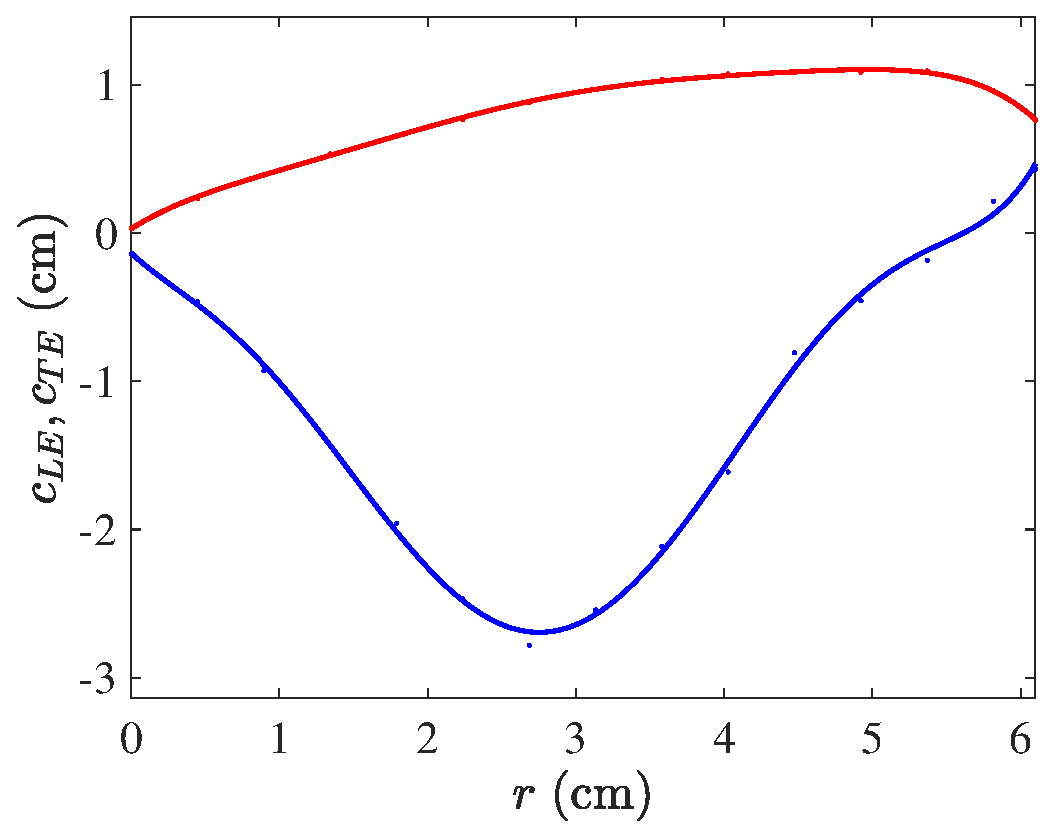
\includegraphics[width=0.45\textwidth]{MONARCH_c_LE_TE}
        }
        \hfill
        \subfigure[Chord $c(r)$]{
            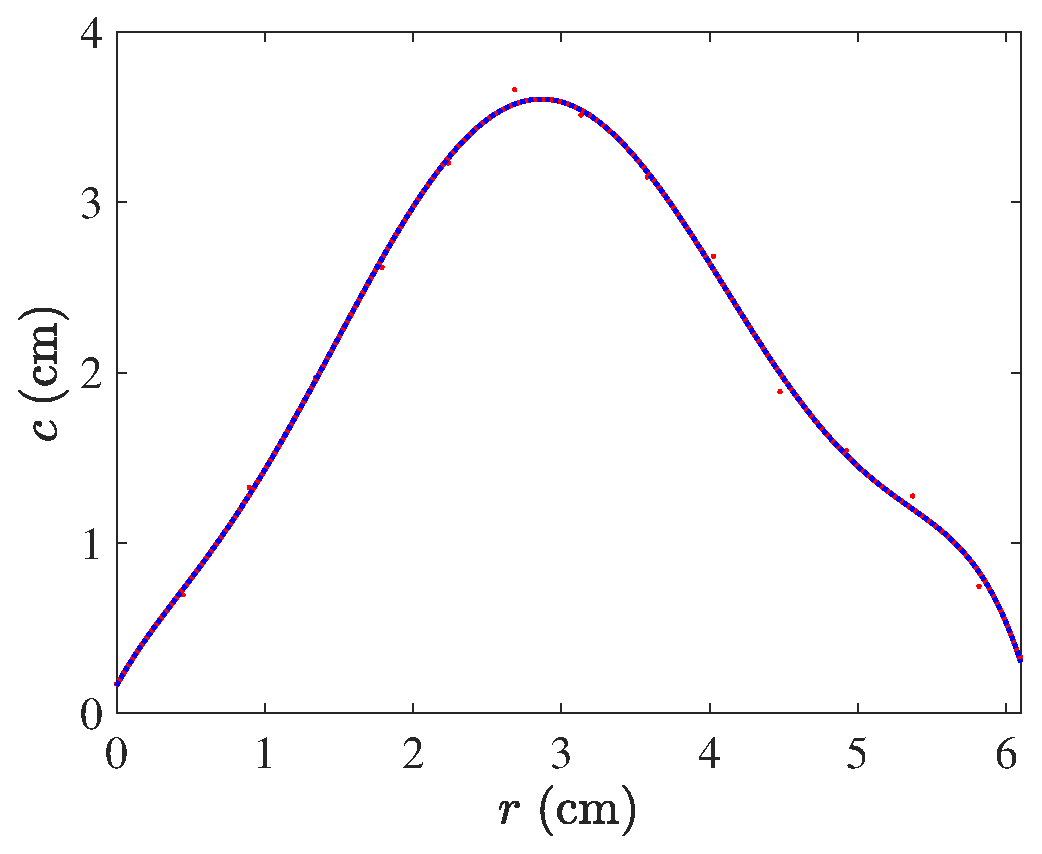
\includegraphics[width=0.45\textwidth]{MONARCH_c}
        }
    }
    \caption{Monarch wing shape and chord}\label{fig:Monarch_wing}
\end{figure}

The morphological parameters and the mass distribution of Monarch are determined by an actual butterfly [ref].
The location of the leading edge and the trailing edge are measured along the span-wise direction, and they are fitted by sixth-order polynomials.  
The resulting measurements and the fitted curve are illustrated in Figure \ref{fig:Monarch_wing}.
From the fitted chord, we determine the morphological parameters as summarized in Table \ref{tab:Monarch}.
\newcolumntype{m}{>{$}l<{$}} % math-mode version of "c" column type
\begin{table}
    \caption{Monarch parameters}\label{tab:Monarch}
    \begin{center}
        \begin{tabular}{|m|m|m|m|m|m|}
            \hline
            \multicolumn{2}{|c}{{Head/Thorax}} & \multicolumn{2}{|c|}{{Abdomen}} & \multicolumn{2}{c|}{{Right Wing}}\\\hline
            m_B & \num{1.485e-4}\,\si{kg} &
            m_A & \num{1.092e-4}\,\si{kg} &    
            m_R & \num{2.5100 e-5}\,\si{kg} \\
            h_B & \num{1.463e-2}\,\si{m} &
            h_A & \num{1.738e-2}\,\si{m} & 
            \bar c & \num{2.0905e-02}\,\si{m} \\
            w_B & \num{5.680e-3}\,\si{m} &
            w_A & \num{3.710e-3}\,\si{m} &
            l & \num{6.0996e-2}\,\si{m}\\
            J_{B_{xx}} & \num{5.9887e-10}\,\si{kgm^2} &
            J_{A_{xx}} & \num{1.8788e-10}\,\si{kgm^2} &  
            J_{R_{xx}} & \num{2.7568e-08}\,\si{kgm^2} \\
            J_{B_{yy}} & \num{2.9481e-09}\,\si{kgm^2} &
            J_{A_{yy}} & \num{1.1089e-08}\,\si{kgm^2} &
            J_{R_{xy}} & \num{2.4957e-09}\,\si{kgm^2} \\
            J_{B_{zz}} & \num{2.9481e-09}\,\si{kgm^2} &
            J_{A_{zz}} & \num{1.1089e-08}\,\si{kgm^2} &
            J_{R_{yy}} & \num{2.5799e-09}\,\si{kgm^2}\\
                       &&&& J_{R_{zz}} & \num{3.0148e-08}\,\si{kgm^2}\\
                       &&&& \nu_{R_x} & \num{-4.4378e-03}\,\si{m} \\
                       &&&& \nu_{R_y} & \num{1.5176e-02}\,\si{m} \\
                       &&&& S &  \num{1.2751e-03}\,\si{m^2} \\ 
                       &&&& \AR & \num{2.9178e+00}\\
                       &&&& \tilde r_1& \num{4.9761e-01}\\
                       &&&& \tilde r_2 & \num{5.4332e-01}\\
                       &&&& \tilde r_3 & \num{5.8030e-01}\\
                       &&&& r_{cp} & \num{6.5148e-02}\,\si{m}\\
                       &&&& \tilde v & \num{1.2496e+00}\\
                       &&&& \tilde r_1(v) & \num{4.8750e-01}\\
                       &&&& \tilde r_2(v) & \num{5.1653e-01}\\
                       &&&& r_\rot & \num{3.3383e-02}\,\si{m}\\ \hline
        \end{tabular}\\[0.1cm]
        (The properties of the left wing are identical to the right wing,  except $\nu_{L_y}= -\nu_{R_y}$, $J_{L_{xy}} = - J_{R_{xy}}$.)
    \end{center}
\end{table}

For the calculation of the inertia matrix, the head/thorax is considered as a cylinder with the height $h_B$ and the diameter $w_B$.
The moment of inertia of the body about its center of gravity is 
\begin{align*}
    J_B & = m_B\, \mathrm{diag} [ \frac{1}{8} w_B^2 , \; \frac{1}{16}w_B^2 + \frac{1}{12}h_B^2, \; \frac{1}{16}w_B^2 + \frac{1}{12} h_B^2] .
\end{align*}
The abdomen is also considered as a cylinder. 
Its moment of inertia about the joint is
\begin{align*}
    J_A & = m_A\, \mathrm{diag} [ \frac{1}{8} w_A^2 ,\;  \frac{1}{16}w_A^2 + \frac{1}{3}h_A^2, \; \frac{1}{16}w_B^2 + \frac{1}{3} h_A^2].
\end{align*}
Next, the right wing is considered as a thin plate with a uniform, negligible thickness. 
The mass element is written as
\[
    dm = \frac{m_R}{S} dx dy,
\]
where $\frac{m_R}{S}$ corresponds to the area density in the unit of \si{kg/m^2}.
Thus, the mass center of the right wing is located at
\begin{align*}
    \nu_{R_x} & = \frac{1}{m_R} \int_{\mathcal{B}_R} x  dm
                = \frac{1}{S} \int_{0}^l \int_{c_{TE}(y)}^{c_{LE}(y)} x dx dy
                = \frac{1}{S} \int_0^l \frac{1}{2}(c_{LE}^2(y)-c_{TE}^2(y)) dy,\\
    \nu_{R_y} & = \frac{1}{m_R} \int_{\mathcal{B}_R} y  dm
                = \frac{1}{S} \int_{0}^l \int_{c_{TE}(y)}^{c_{LE}(y)} y dx dy
                = \frac{1}{S} \int_0^l (c_{LE}(y)-c_{TE}(y))y dy.
\end{align*}
Thus, the moment of inertia about the wing root is given by
\begin{align*}
    J_{R_{xx}} & = \int_{\mathcal{B}_R} y^2 dm 
                = \frac{m_R}{S} \int_{0}^l \int_{c_{TE}(y)}^{c_{LE}(y)} y^2 dx dy
                = \frac{m_R}{S} \int_0^l y^2(c_{LE}(y)-c_{TE}(y)) dy,\\
    J_{R_{xy}} & = \int_{\mathcal{B}_R} -x y dm 
                = \frac{m_R}{S} \int_{0}^l \int_{c_{TE}(y)}^{c_{LE}(y)} -xy dx  dy
                = \frac{m_R}{S} \int_0^l -\frac{1}{2}(c_{LE}^2(y)-c_{TE}^2(y))y dy,\\
    J_{R_{yy}} & = \int_{\mathcal{B}_R} x^2 dm 
                = \frac{m_R}{S} \int_{0}^l \int_{c_{TE}(y)}^{c_{LE}(y)} x^2 dx  dy
                = \frac{m_R}{S} \int_0^l \frac{1}{3}(c_{LE}^3(y)-c_{TE}^3(y)) dy,\\
                J_{R_{zz}} & = J_{R_{xx}} + J_{R_{yy}}.
\end{align*}
Similarly, for the left wing, we have
\begin{align*}
    J_{L_{xx}} & = \frac{m_R}{S} \int_0^{-l} \int_{c_{TE}(-y)}^{c_{LE}(-y)} y^2 dx dy = J_{R_{xx}} \\
    J_{L_{xy}} & = \frac{m_R}{S} \int_0^{-l} \int_{c_{TE}(-y)}^{c_{LE}(-y)} -xy dx dy = - J_{R_{xy}} \\
    J_{L_{yy}} & = \frac{m_R}{S} \int_0^{-l} \int_{c_{TE}(-y)}^{c_{LE}(-y)} x^2 dx dy = J_{R_{xx}} \\
    J_{L_{zz}} & = J_{R_{zz}}.
\end{align*}
Finally, it is assumed that the root of the wing and the joint of the abdomen are located at
\begin{align*}
    \mu_R = [0,\; \frac{w_B}{2},\; 0],\\
    \mu_L = [0,\; -\frac{w_B}{2},\; 0],\\
    \mu_A = [-\frac{h_B}{2},\; 0,\; 0].
\end{align*}

\subsection{Flight Characteristics of Monarch}

The flight of an actual Monarch butterfly is studied by a motion capture system. 
The twelve markers are attached to a Monarch as illustrated in Figure \ref{fig:Monarch_marker},
and the position of each marker is measured by a VICON motion capture system at 200\si{Hz}.

\begin{figure}
    \centerline{
        \subfigure[Marker location]{
            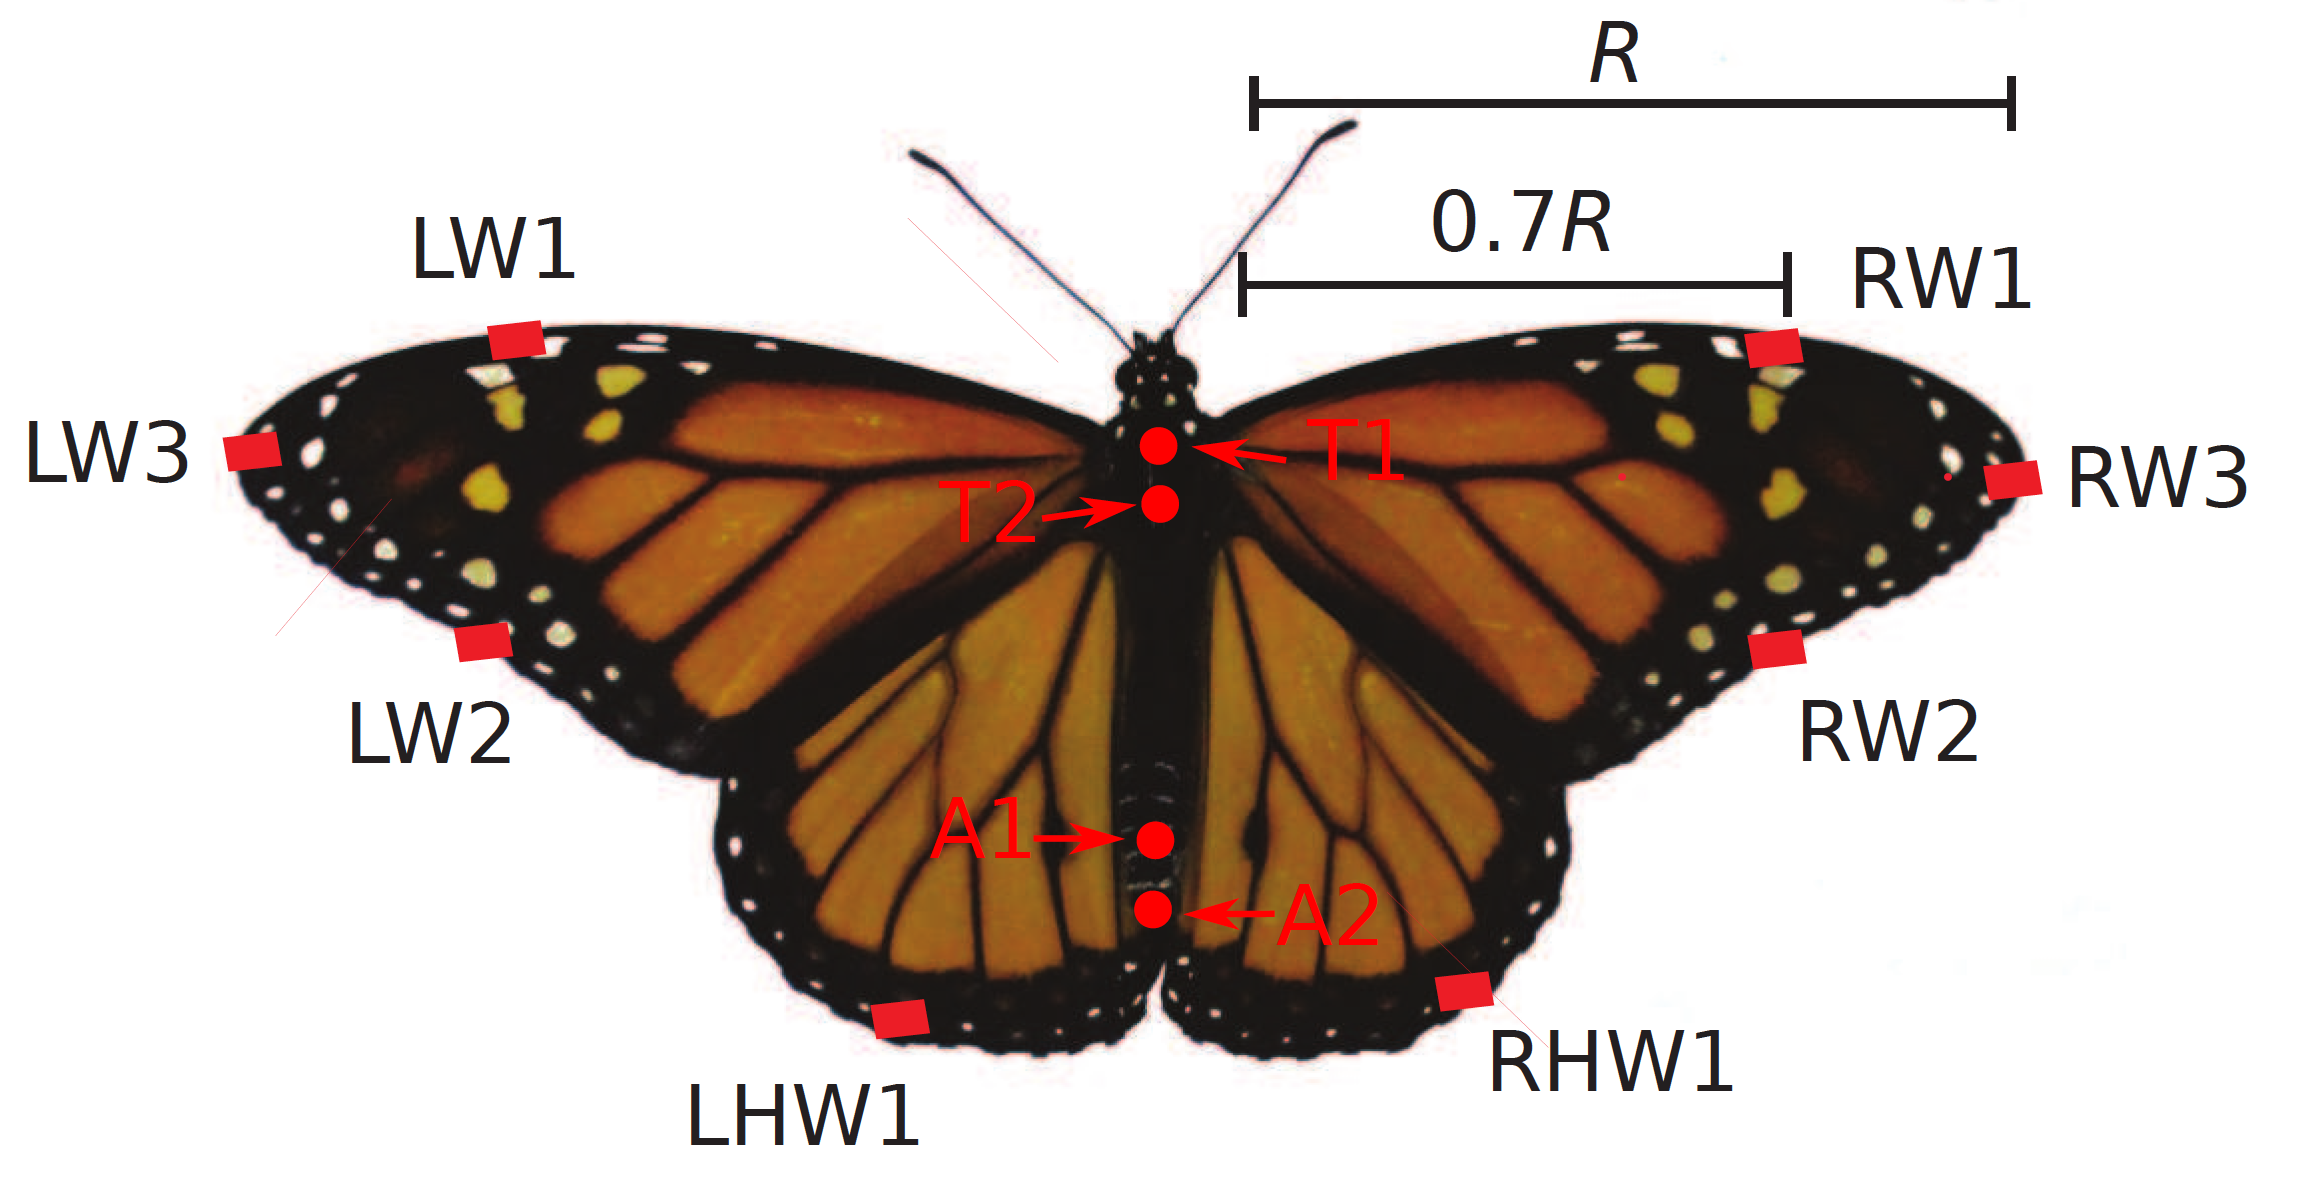
\includegraphics[width=0.5\textwidth]{Monarch_marker}
        }
        \hfill
        \subfigure[Monarch object reconostructed by markers]{
            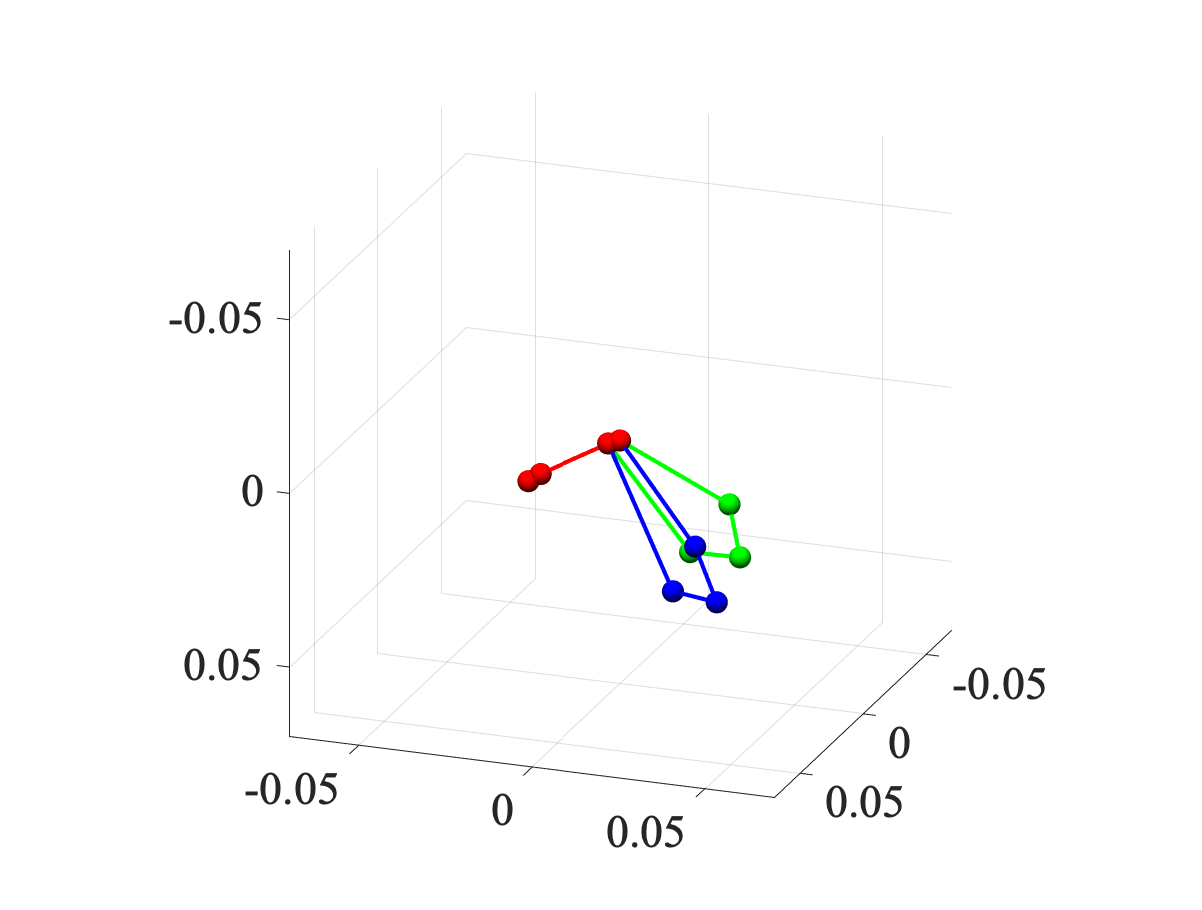
\includegraphics[width=0.5\textwidth]{Monarch_frame}
        }
}
\caption{Monarch motion capture}\label{fig:Monarch_marker}
\end{figure}


These are converted into $(x,R,Q_R,Q_L,Q_A)$ as follows. 
It is considered that the origin of the body, namely $x$ is located at the center of $T_1$ and $T_2$. 
For the body attitude $R$, it is assumed that the first axis is along $T_1-T_2$ and the second axis is parallel to the ground, i.e., there is no body roll. 
This is reasonable as the measured flight trajectory is almost straight. 
For the attitude of the abdomen, the first axis points from the center of $A_1$ and $A_2$ toward $T_2$, and the second axis is parallel to the ground. 
The resulting rotation matrix is left multiplied by $R^T$ to obtain the relative attitude $Q_A$. 

For the right wing attitude, it is assumed that the wing root it located at the center of $T_1$ and $T_2$.
The wing plane always passes through the wing root exactly, and it is spanned by the three markers on the right wing. 
However, due to the measurement errors and the flexibility of the wing, those points do not exactly lie on a single plane. 
Instead, we find the normal vector of the plane such that the sum of the squared distance between each marker and the plane is minimized. 
The normal vector yields the third axis of $\mathcal{F}_R$. 
For the second axis, the vector from the wing root to $RW_3$ is projected on to the fitted plane. 
The first axis is determined by the cross product of the second axis and the third axis. 
These yield the rotation matrix of the right wing from the inertial frame, and by left multiplying $R^T$, we obtain $Q_R$. 
The attitude of the left wing, namely $Q_L$ is constructed similarly. 

Next, the computed $(Q_R(t),Q_L(t))$ are converted into wing kinematics angles as follows. 
First, we determine the wing stroke plane. 
In the absences of the deviation angle $\psi$, the second column of $Q_R(t)$ and $Q_L(t)$ over multiple time instances span the stroke plane. 
We find the stroke plane such that the sum of the squared distance for $Q_R(t) e_2$ and $Q_L(t) e_2$ for varying $t$ over the experiment period is minimized. 
It turns out that the normal vector to the stroke plane is not in the $\mathbf{b}_x$--$\mathbf{b}_z$ plane. 
More explicitly, it is given by $[   -0.8948, -0.1222, 0.4294]$, i.e., it is rotated by $-7.77\si{deg}$ when observed the dorsal side,
or the right wing tip is ahead of the left wing tip.
This might have been caused by the asymmetry of the particular Monarch butterfly used in the experiment, or the bias in the marker attachment.
Instead dealing with the asymmetry in the left wing and the right wing, we multiply $\exp(7.77\hat e_3)$ to $Q_R$ and $Q_L$ such that they become symmetric in the least square sense. 
The resulting normal vector of the stroke plane lies in the $\mathbf{b}_x$--$\mathbf{b}_z$ plane, ans the stroke plane angle is $\beta = 25.42\si{deg}$.
From the given $\beta$, and rotated $Q_R(t),Q_L(t)$, we can determine the wing kinematics angles $(\phi_R(t),\theta_R(t),\psi_R(t)$, and $(\phi_L(t),\theta_L(t),\psi_L(t))$ according to \eqref{eqn:Q_R} and \eqref{eqn:Q_L}, respectively. 
These are illustrated in Figure \ref{fig:Monarch_WK}.
The wing kinematics angles for the right wing are mostly consistent withe the left wing, except the small deviation angle. 
Assuming the symmetric wing kinematics, we take the average between the right wing and the left wing, 
and they are fitted with Fourier series to be used in the subsequent dynamic simulation. 


\begin{figure}
    \centerline{
        \subfigure[wing tip locations]{
            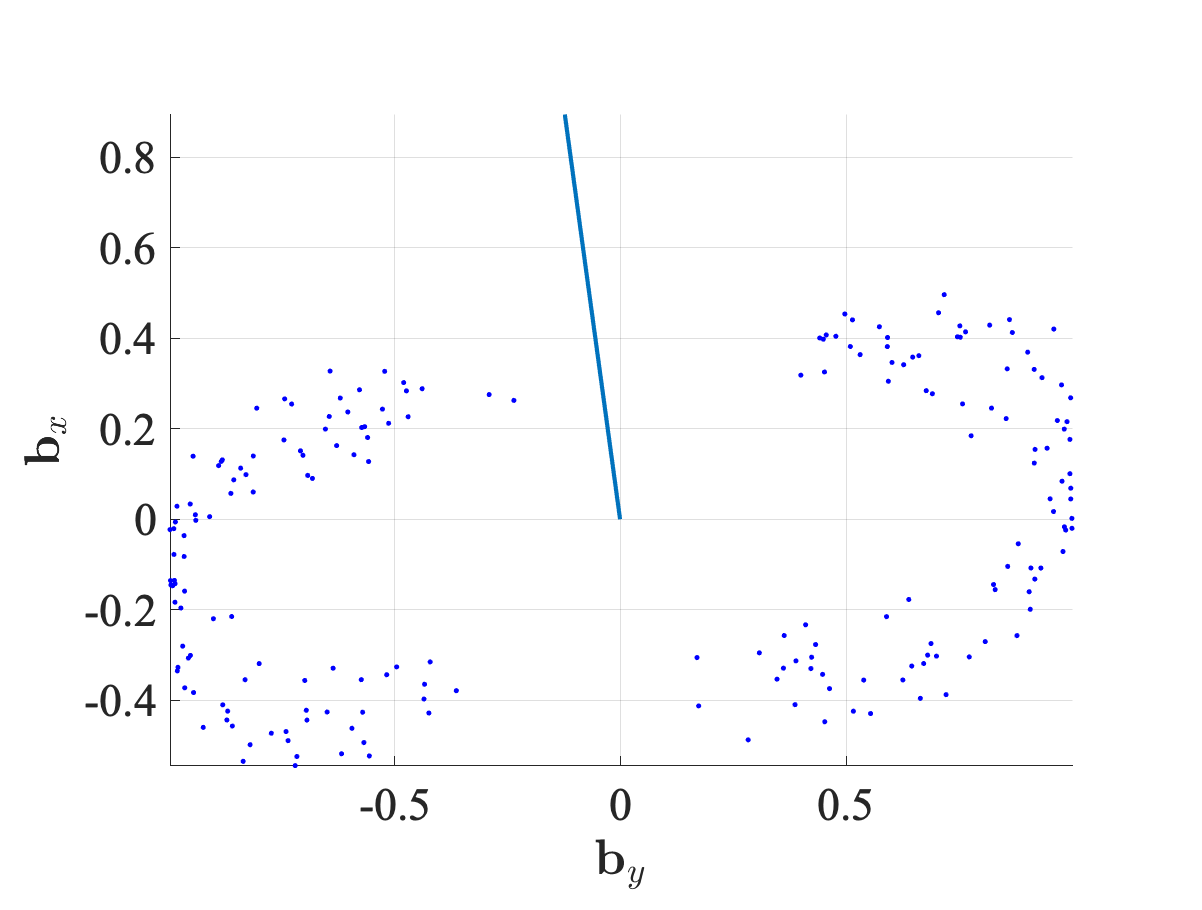
\includegraphics[width= 0.45\textwidth]{fit_VICON_wing_tip}
        }
        \hfill
        \subfigure[wing kinematics angles]{
            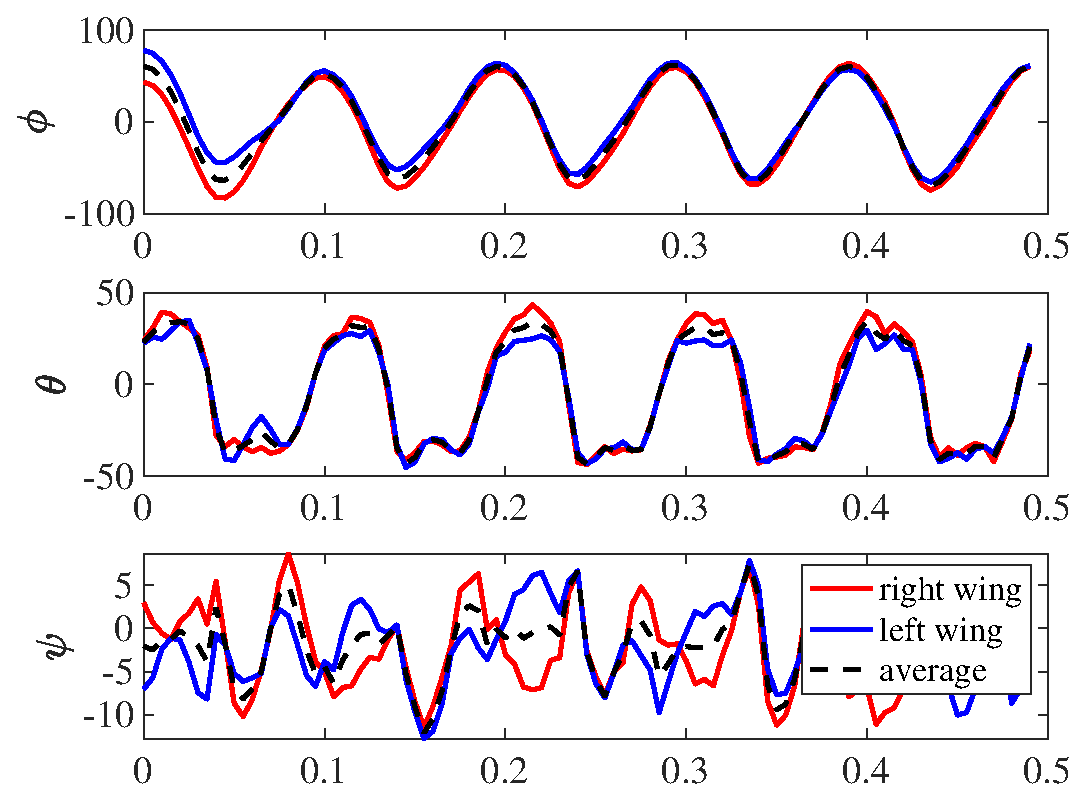
\includegraphics[width= 0.45\textwidth]{fit_VICON_E}
        }
    }
    \caption{Monarch wing kinematics}\label{fig:Monarch_WK}
\end{figure}

\subsection{Dynamic Simulation}

From the above wing kinematics angles and the body/abdomen attitude obtained by the actual Monarch butterfly,
we numerically integrate the quasi-steady position dynamics, namely \eqref{eqn:mx_ddot}.
The corresponding results are compared against the experimental data. 
These are illustrated at Figure \ref{fig:comp_VICON}.
In general, the downstrokes generate the lift upward, and the upstrokes generate thrust forward,
while yielding a climbing trajectory with oscillation.

The QS model generates greater lift and thrust, and consequently causing higher climb rate and forward velocity. 
However, it is consistent with the experimental data in a qualitative sense. 


\begin{figure}[p]
    \centerline{
        \subfigure[Position trajectory]{
            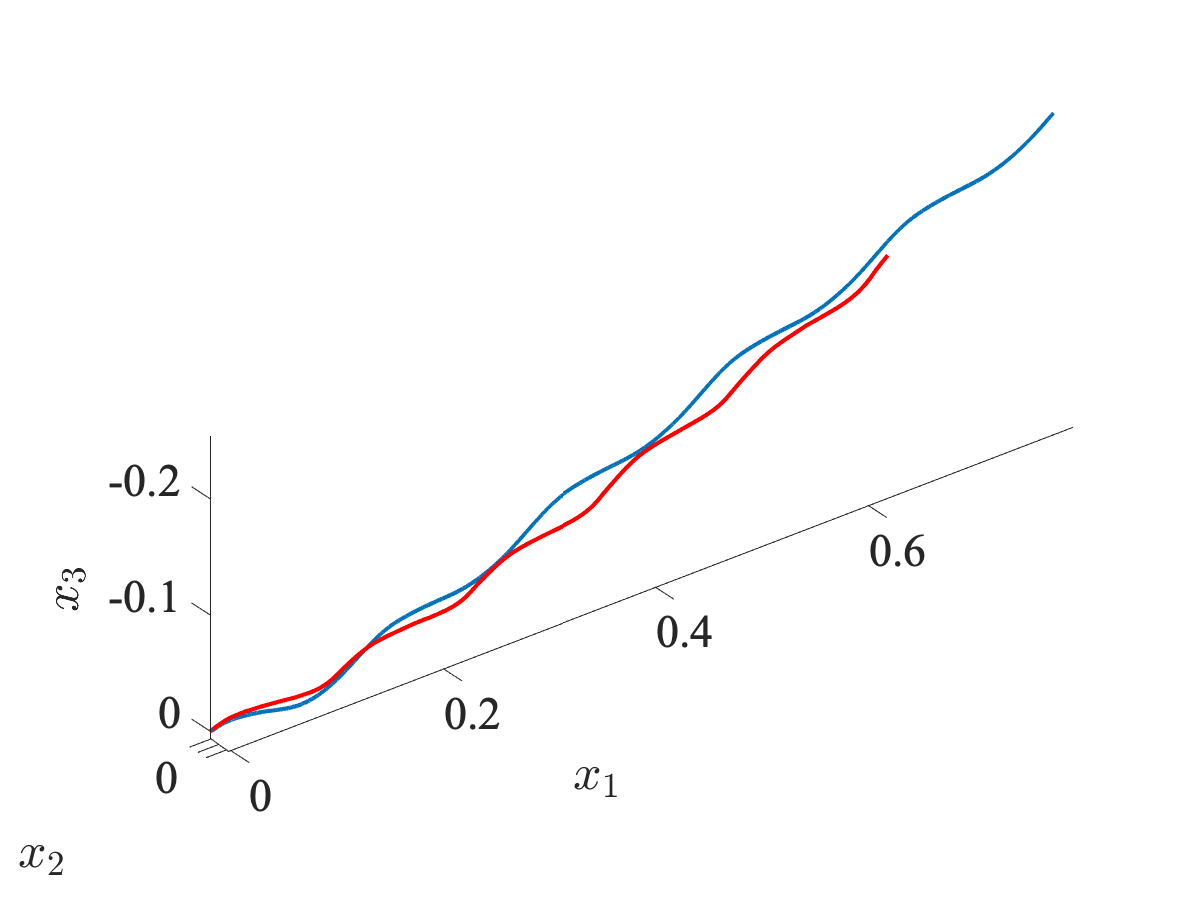
\includegraphics[width=0.5\textwidth]{comp_VICON_x3}
        }
        \hfill
        \subfigure[Position $x$]{
            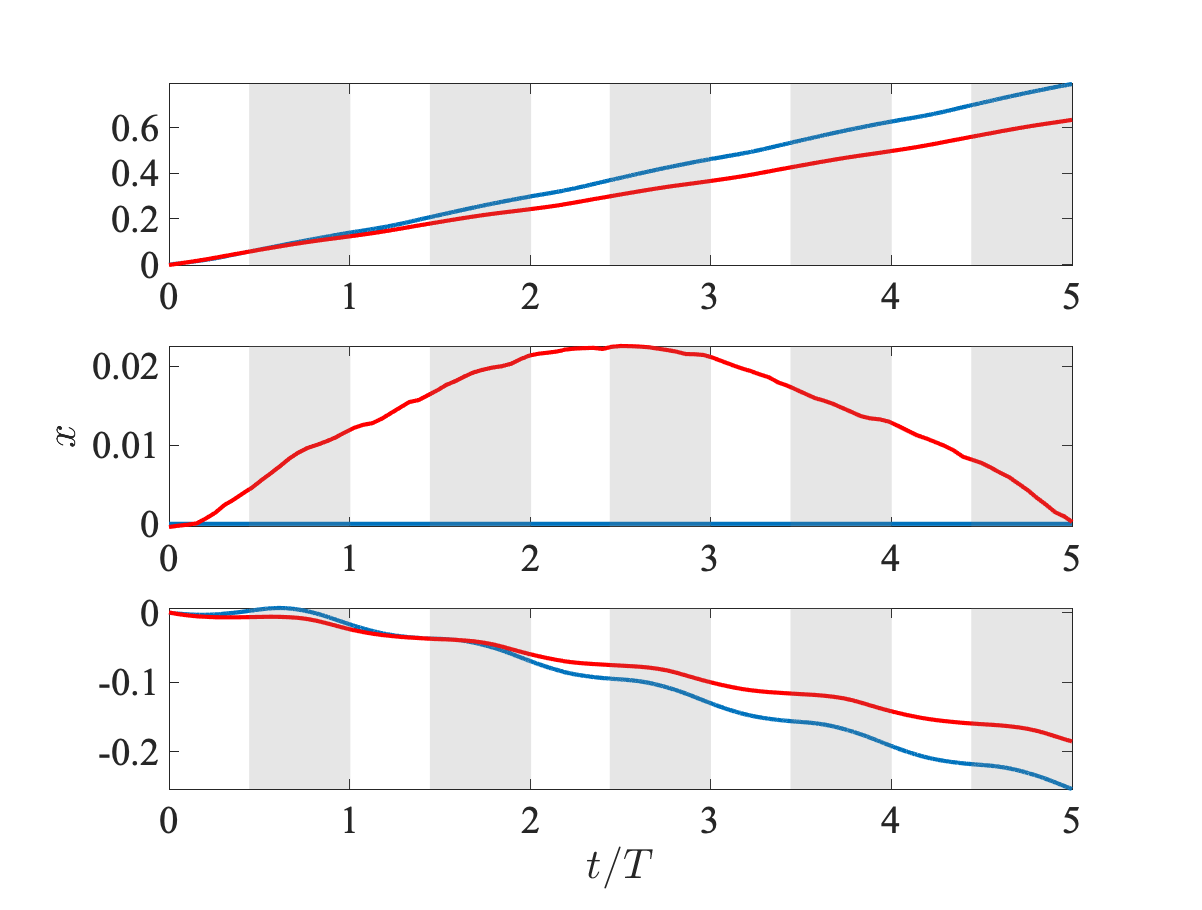
\includegraphics[width=0.5\textwidth]{comp_VICON_x}
        }
    }
    \centerline{
        \subfigure[Velocity $\dot x$]{
            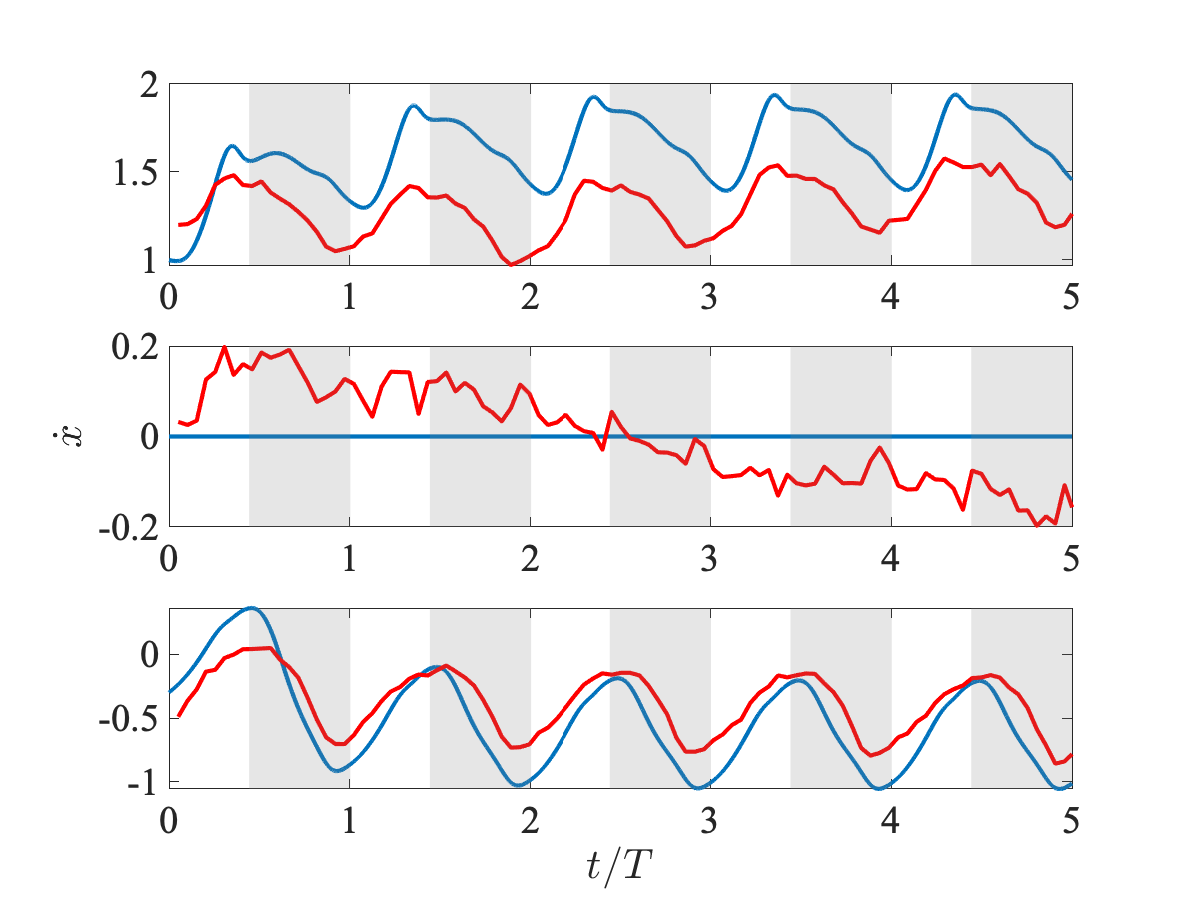
\includegraphics[width=0.5\textwidth]{comp_VICON_v}
        }
        \hfill
        \subfigure[Resultant force in the body-fixed frame]{
            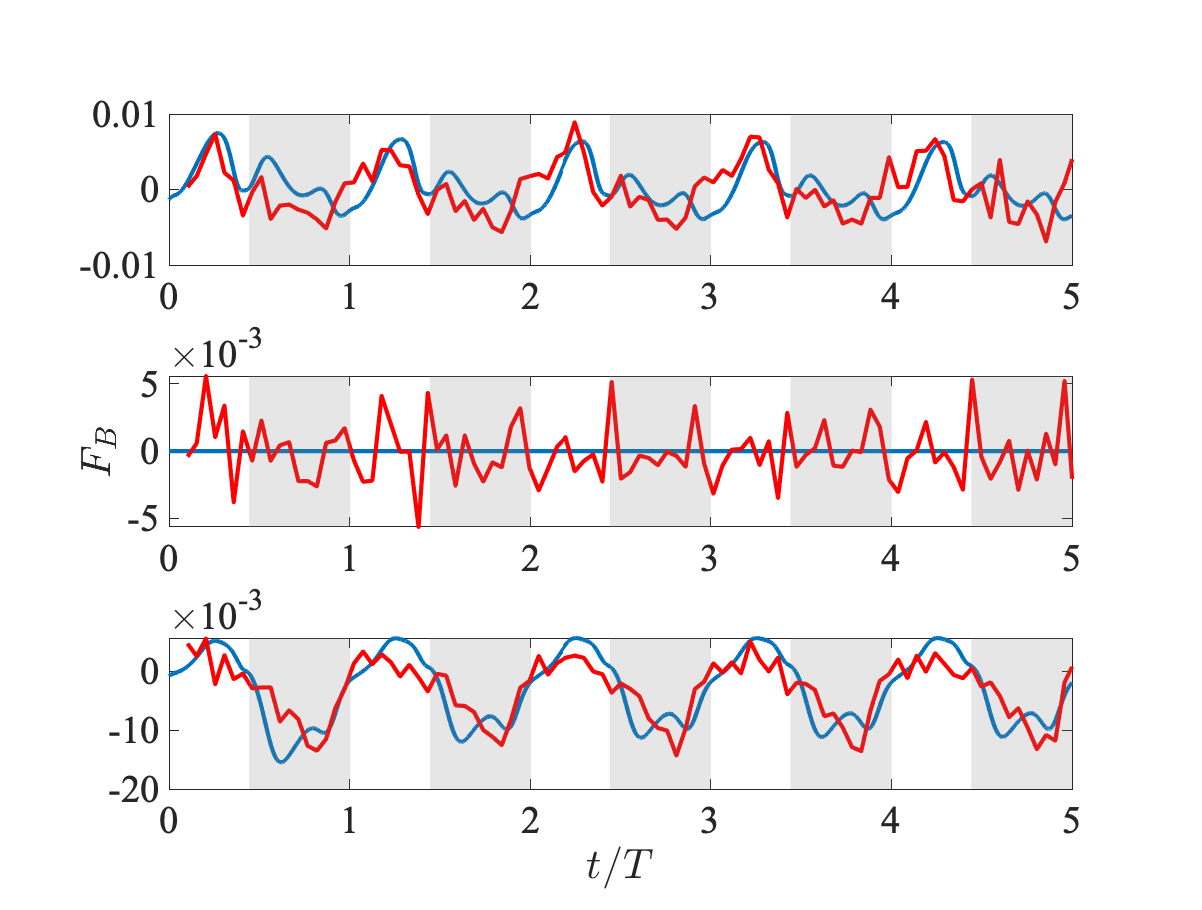
\includegraphics[width=0.5\textwidth]{comp_VICON_FB}
        }
    }
    \centerline{
        \subfigure[Wing kinematics angles]{
            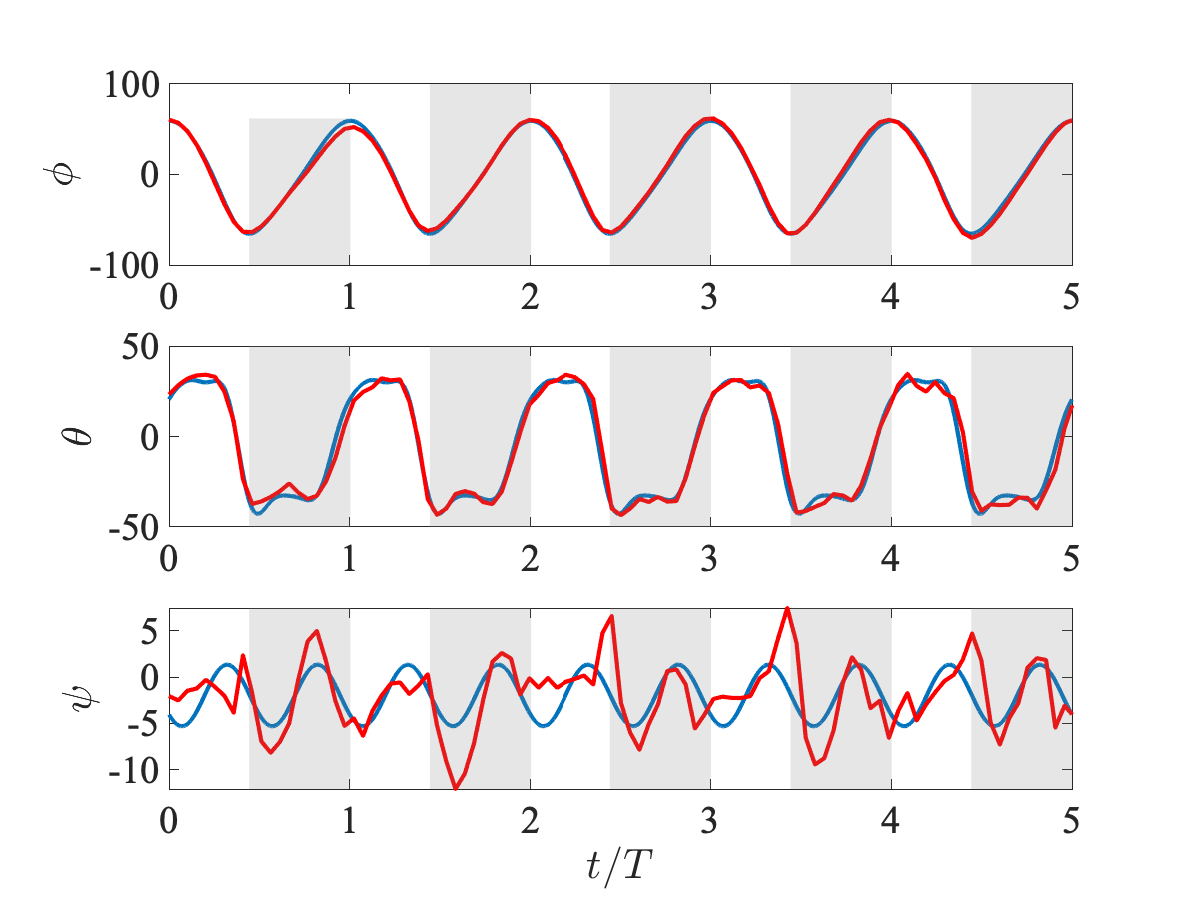
\includegraphics[width=0.5\textwidth]{comp_VICON_E}
        }
        \hfill
        \subfigure[Body pitch / Abdomen relative pitch]{
            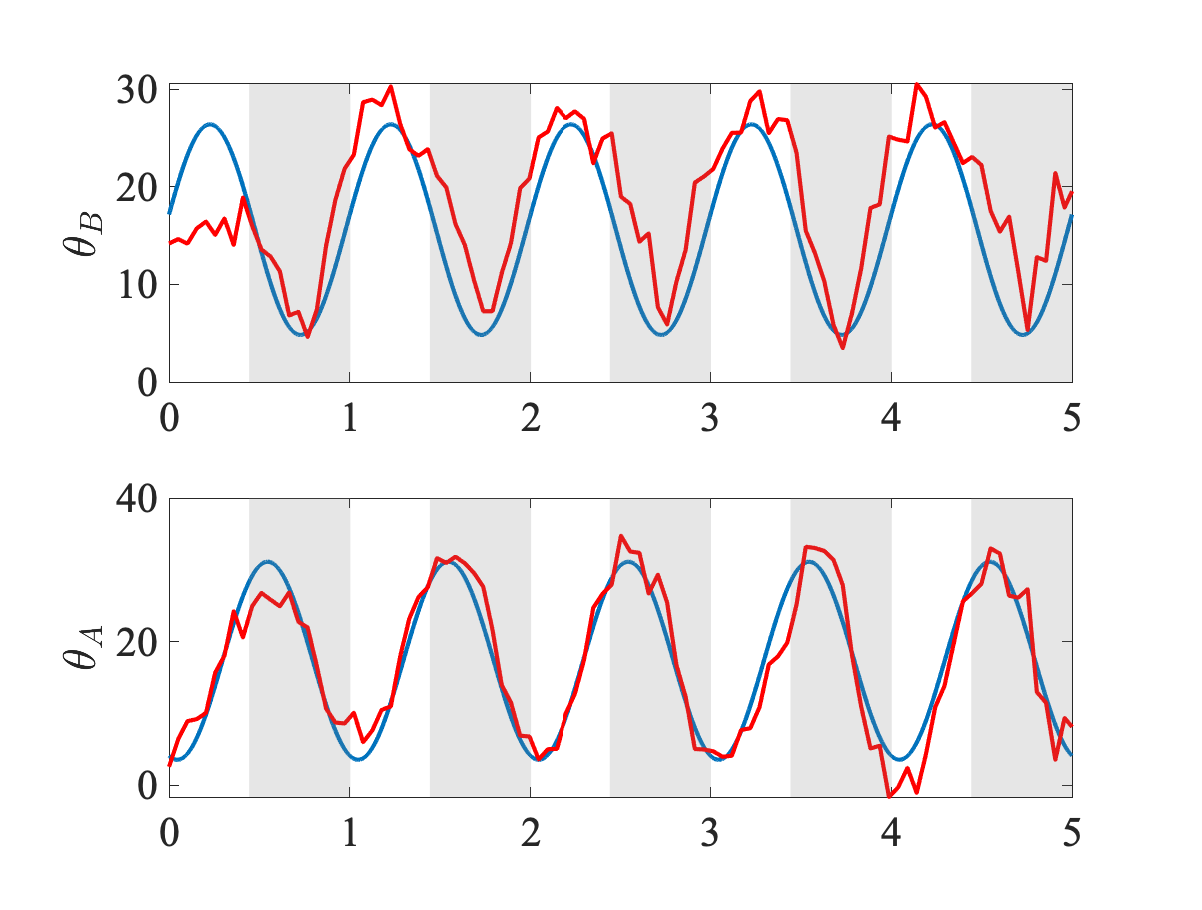
\includegraphics[width=0.5\textwidth]{comp_VICON_theta}
        }
    }
    \caption{Comparison between the QS model (blue) and the experimental data (red); shaded area corresponds to downstroke; the resultant force of the experiment is constructed by the acceleration of the thorax, multiplied by the total mass and subtracted by the gravity}\label{fig:comp_VICON}
\end{figure}

\subsection{Effects of Abdomen}

In Monarch butterfly flights, the abdomen oscillate at the same frequency of the wing flapping angle with the opposite phase,
i.e., the abdomen rotates downward during the wing upstrokes. 


To test the effects of abdomen undulation with the proposed QS model, we simulate the above Monarch model for 50 strokes while fixing the abdomen pitching angle to the averaged value. 
These results are illustrated at Figure \ref{fig:comp_ab}.
While the discrepancy is not substantial, it is shown that the abdomen undulation slightly increases the climb rate and the forward velocity.  
Furthermore, an abdomen undulation in the opposite phase reduces those. 

\begin{figure}[p]
    \centerline{
        \subfigure[Position trajectory]{
            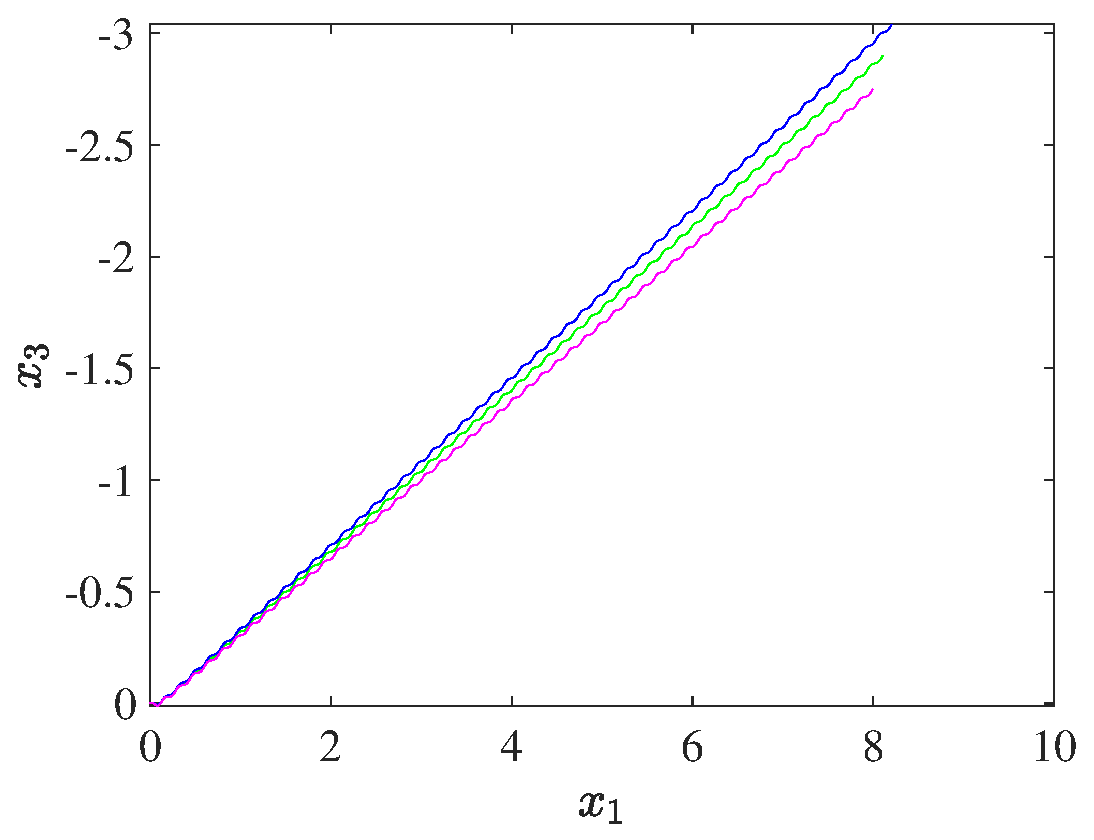
\includegraphics[width=0.5\textwidth]{comp_ab_x3}
        }
        \hfill
        \subfigure[Position $x$]{
            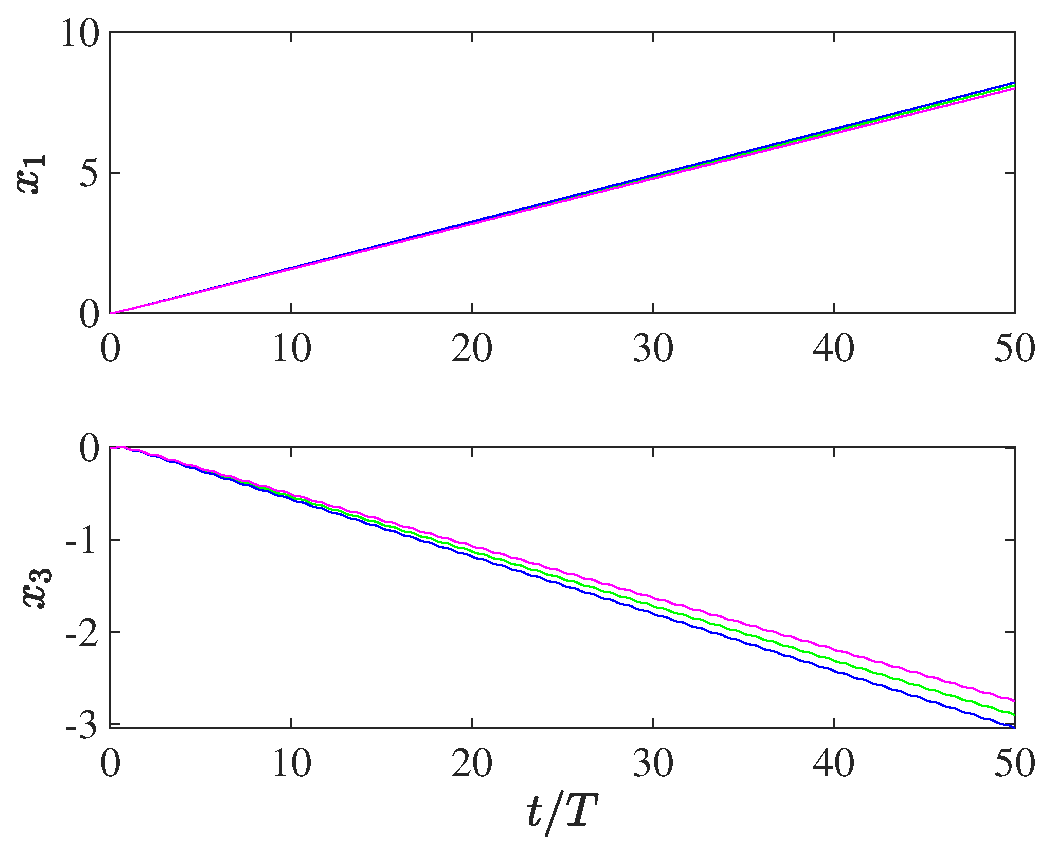
\includegraphics[width=0.5\textwidth]{comp_ab_x}
        }
    }
    \centerline{
        \subfigure[Velocity trajectory]{
            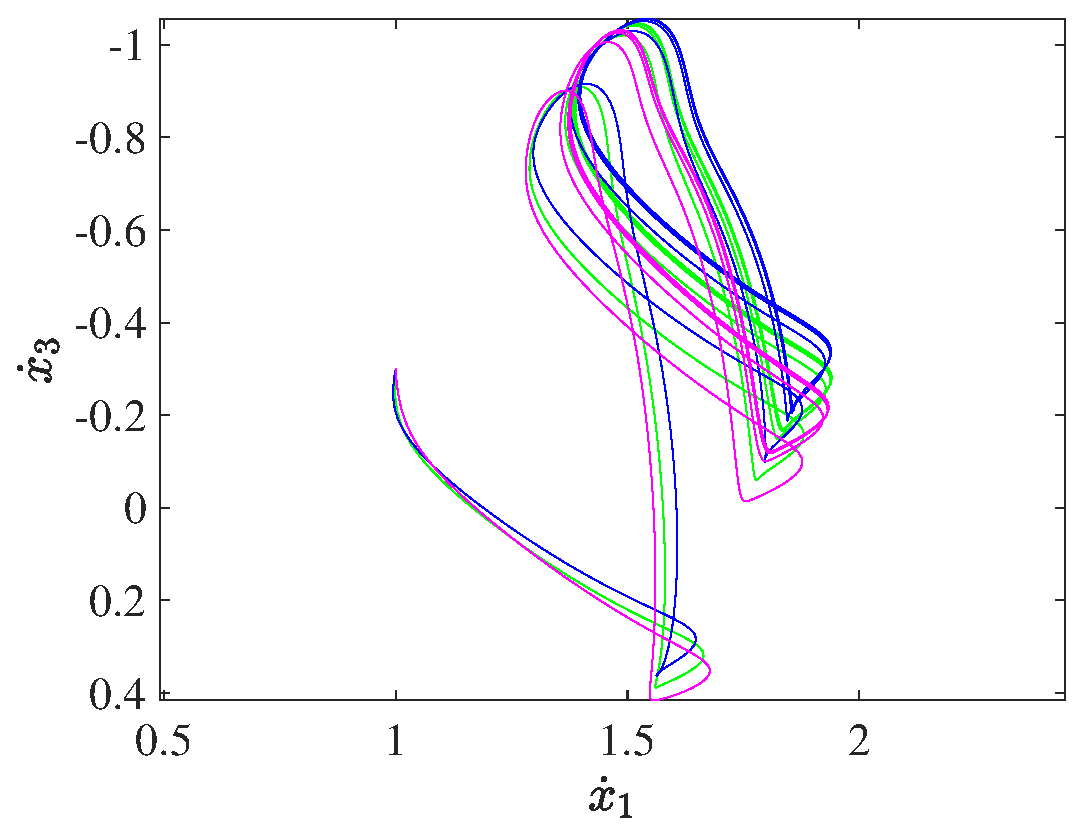
\includegraphics[width=0.5\textwidth]{comp_ab_v3}
        }
        \hfill
        \subfigure[Velocity $\dot x$ (for the first 5 strokes)]{
            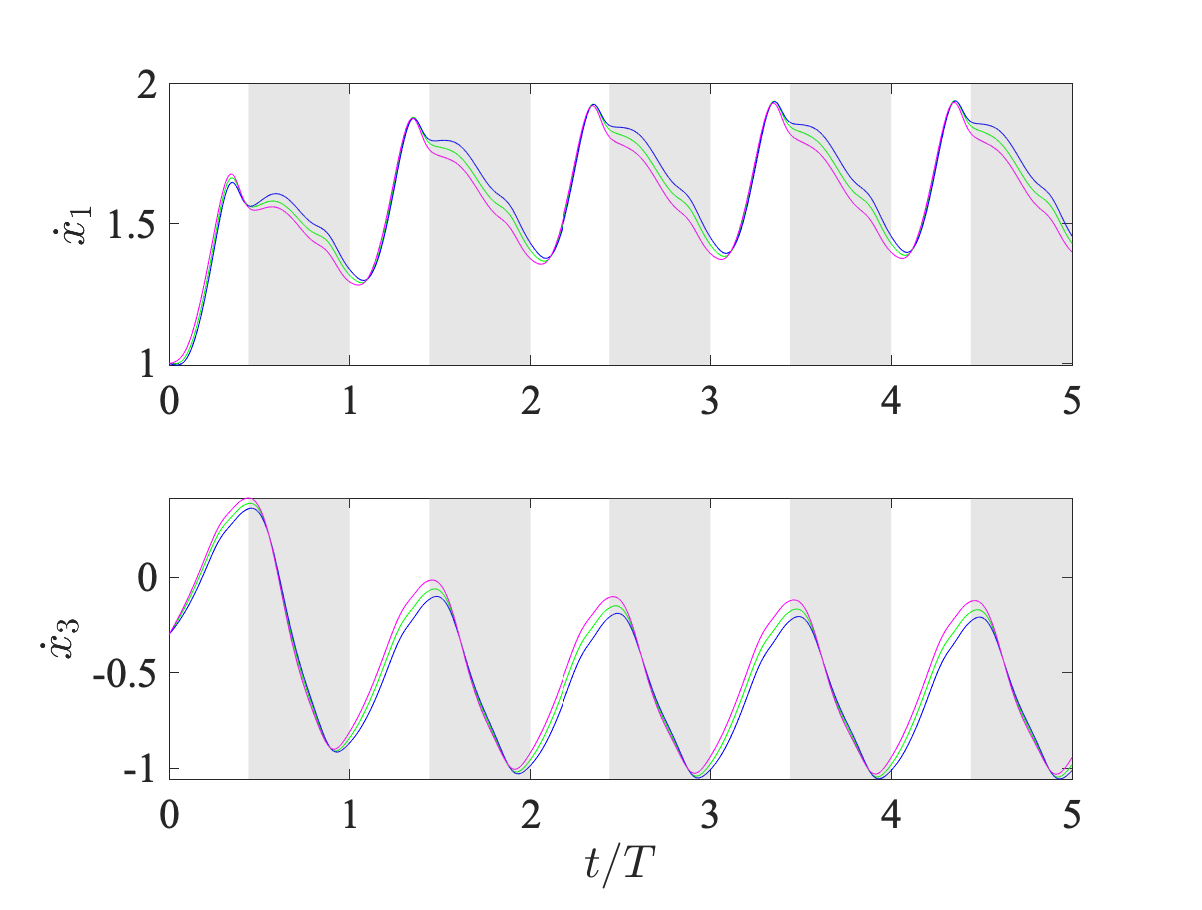
\includegraphics[width=0.5\textwidth]{comp_ab_v}
        }
    }
    \centerline{
        \subfigure[thorax pitch / abdomen pitch (for the first 5 strokes)]{
            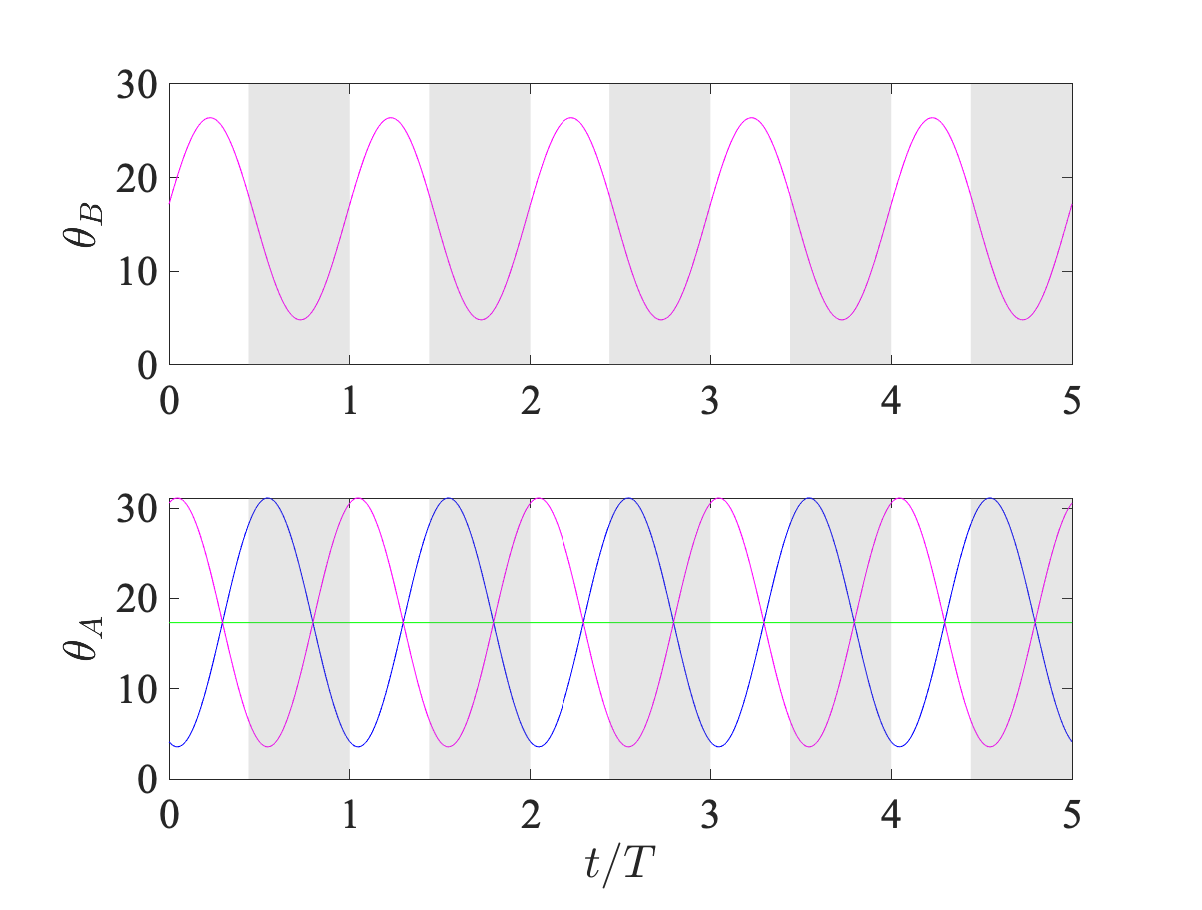
\includegraphics[width=0.5\textwidth]{comp_ab_theta}
        }
    }
    \caption{Comparison between flight with abdomen undulation (blue), without abdomen undulation (green), with abdomen undulation in the opposite phase (purple); the simulation is for 50 strokes, and the results of the first 5 strokes are illustrated for the subfigure (d) and (e)}\label{fig:comp_ab}
\end{figure}

\subsection{Asymptotic Stability}

Another interesting results of Figure \ref{fig:comp_ab}.(c) is that the trajectory of the velocity asymptotically converges to a periodic orbit.  
This suggests that the flapping motion captured by the Monarch butterfly yields an asymptotically stable periodic solution. 
This should be further investigated by dynamic system theory such as Floquet's theorem. 

\subsection{Open-Source Software Package}

A software package for the proposed quasi-state dynamic model of a flapping wing UAV has been developed in Matlab, and it is shared as an open-source library at \href{https://github.com/fdcl-gwu/FWUAV}{\texttt{https://github.com/fdcl-gwu/FWUAV}}.

\begin{itemize}
    \item Morphological parameters of Monarch butterfly are defied at \texttt{morp\_MONARCH.m}
    \item The raw data from VICON are processed by the following three files under \texttt{/exp\_data}.

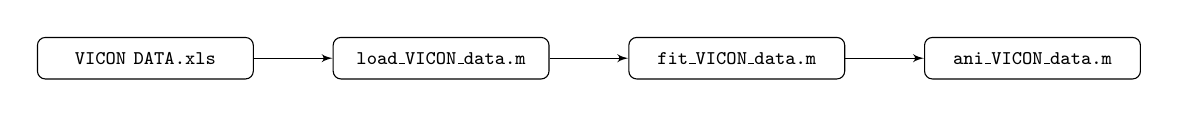
\begin{tikzpicture}[auto]
    \tikzstyle{block} = [text width=7em, draw, rectangle, text centered, rounded corners=1mm, minimum height=1.5em, inner sep= 4pt, style={font=\scriptsize}];
    \tikzstyle{line} = [draw, -latex'];
    \matrix[column sep=10mm, row sep=4mm]
    {
        \node[block] (VICON) {\texttt{VICON DATA.xls}}; & 
            \node[block] (load) {\texttt{load\_VICON\_data.m}}; & 
                \node[block] (fit) {\texttt{fit\_VICON\_data.m}}; & 
                    \node[block] (ani) {\texttt{ani\_VICON\_data.m}}; \\
    };
    \tikzstyle{every path}=[line]
    \path (VICON) -- (load);
    \path (load) -- (fit);
    \path (fit) -- (ani);
\end{tikzpicture}

    \item For given torque at the wing and the abdomen, the complete dynamics \eqref{eqn:EL} are simulated as follows. 

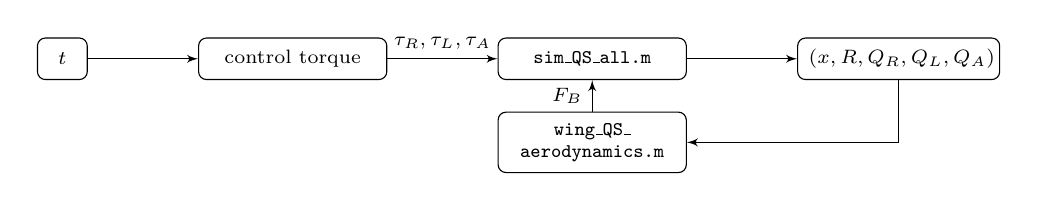
\begin{tikzpicture}[auto]
    \tikzstyle{block} = [text width=6em, draw, rectangle, text centered, rounded corners=1mm, minimum height=1.5em, inner sep= 4pt, style={font=\scriptsize}];
    \tikzstyle{line} = [draw, -latex'];
    \matrix[column sep=14mm, row sep=4mm]
    {
            \node[block,text width=1em] (t) {$t$}; &
        \node[block] (tau) {control torque}; & 
            \node[block] (sim) {\texttt{sim\_QS\_all.m}}; &
        \node[block, text width=6.5em] (output) {$(x,R,Q_R,Q_L,Q_A)$}; \\
            & & \node[block] (QS) {\texttt{wing\_QS\_ aerodynamics.m}}; \\
            %& & \node[block] (QS) {\texttt{wing\_QS\_ aerodynamics.m}};\\
    };
    \tikzstyle{every path}=[line]
    \path (t) -- (tau);
    \path (tau) -- node {\scriptsize $\tau_R,\tau_L,\tau_A$} (sim);
    \path (sim) -- (output);
    \path (output) |- (QS);
    \path (QS) -- node {\scriptsize $F_B$} (sim);
\end{tikzpicture}

    \item For given wing Euler angles and the abdomen attitude, the position and the attitude dynamics of the thorax, namely \eqref{eqn:EL_xR} are simulated as follows.

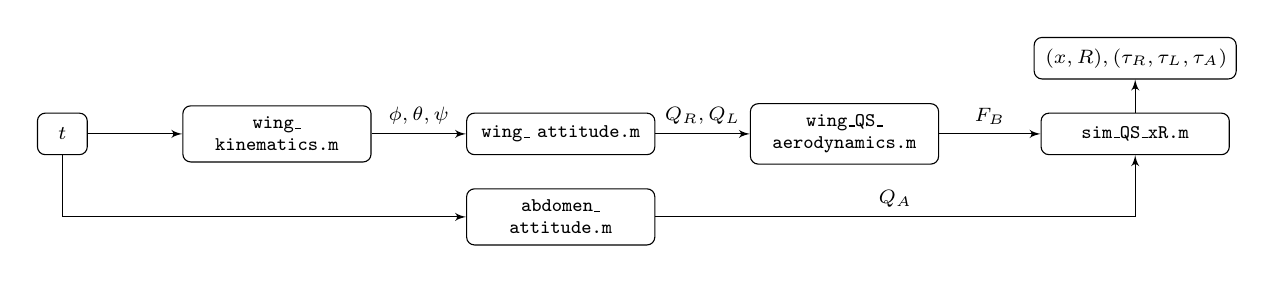
\begin{tikzpicture}[auto]
    \tikzstyle{block} = [text width=6em, draw, rectangle, text centered, rounded corners=1mm, minimum height=1.5em, inner sep= 4pt, style={font=\scriptsize}];
    \tikzstyle{line} = [draw, -latex'];
    \matrix[column sep=12mm, row sep=3mm]
    {
        & & & & 
        \node[block, text width=6.5em] (output) {$(x,R),(\tau_R,\tau_L,\tau_A)$}; \\
        \node[block,text width=1em] (t) at (0,0) {$t$}; &
        \node[block] (wk) {\texttt{wing\_ kinematics.m}}; & 
        \node[block] (wa) {\texttt{wing\_ attitude.m}}; &
            \node[block] (QS) {\texttt{wing\_QS\_ aerodynamics.m}}; &
        \node[block] (sim_x) {\texttt{sim\_QS\_xR.m}}; \\
            & &
        \node[block] (aa) {\texttt{abdomen\_ attitude.m}}; \\
    };
    \tikzstyle{every path}=[line]
    \path (t) -- (wk);
    \path (t) |- (aa);
    \path (wk) -- node {\scriptsize $\phi,\theta,\psi$} (wa);
    \path (wa) -- node {\scriptsize$Q_R,Q_L$} (QS);
    \path (QS) -- node {\scriptsize$F_B$} (sim_x);
    \path (aa) -| node[near start] {\scriptsize $Q_A$} (sim_x);
    \path (sim_x) -- (output);
\end{tikzpicture}

    \item For given wing Euler angles, the thorax attitude, and the abdomen attitude, the position dynamics \eqref{eqn:mx_ddot} are simulated as follows.

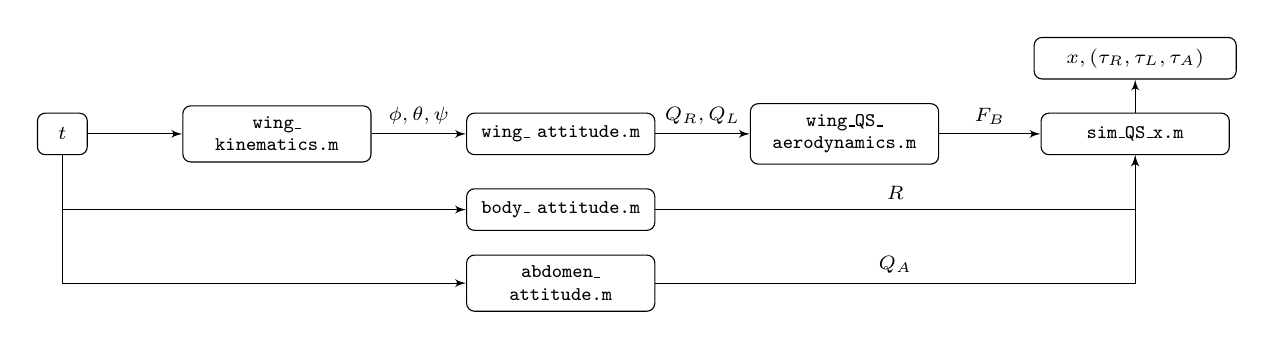
\begin{tikzpicture}[auto]
    \tikzstyle{block} = [text width=6em, draw, rectangle, text centered, rounded corners=1mm, minimum height=1.5em, inner sep= 4pt, style={font=\scriptsize}];
    \tikzstyle{line} = [draw, -latex'];
    \matrix[column sep=12mm, row sep=3mm]
    {
        & & & & 
        \node[block, text width=6.5em] (output) {$x,(\tau_R,\tau_L,\tau_A)$}; \\
        \node[block,text width=1em] (t) at (0,0) {$t$}; &
        \node[block] (wk) {\texttt{wing\_ kinematics.m}}; & 
        \node[block] (wa) {\texttt{wing\_ attitude.m}}; &
            \node[block] (QS) {\texttt{wing\_QS\_ aerodynamics.m}}; &
        \node[block] (sim_x) {\texttt{sim\_QS\_x.m}}; \\
            & &
        \node[block] (ba) {\texttt{body\_ attitude.m}}; \\
            & &
        \node[block] (aa) {\texttt{abdomen\_ attitude.m}}; \\
    };
    \tikzstyle{every path}=[line]
    \path (t) -- (wk);
    \path (t) |- (ba);
    \path (t) |- (aa);
    \path (wk) -- node {\scriptsize $\phi,\theta,\psi$} (wa);
    \path (wa) -- node {\scriptsize$Q_R,Q_L$} (QS);
    \path (QS) -- node {\scriptsize$F_B$} (sim_x);
    \path (ba) -| node[near start] {\scriptsize$R$} (sim_x);
    \path (aa) -| node[near start] {\scriptsize $Q_A$} (sim_x);
    \path (sim_x) -- (output);
\end{tikzpicture}
\end{itemize}


\bibliographystyle{IEEEtran}
\bibliography{FWUAV,/Users/tylee/Documents/BibMaster17.bib,/Users/tylee/Documents/tylee.bib,BibCK}

\appendix

\subsection*{Appendix}

\subsubsection*{Hat Map}

For $x=(x_1,x_2,x_3)\in\Re^3$, 
\begin{align}
    \hat x = \begin{bmatrix}
        0 & -x_3 & x_2 \\
        x_3 & 0 & -x_1 \\
        -x_2 & x_1 & 0 
    \end{bmatrix},
\end{align}


\subsubsection*{Sign Function}

For $x\in\Re$, 
\begin{align}
    \mathrm{sgn}(x) =
    \begin{cases}
        1 &  x>0,\\
        0 &  x=0,\\
        -1 & x<0.
    \end{cases}
\end{align}

\clearpage\newpage
\KOMAoptions{paper=landscape,pagesize}
\recalctypearea

\subsubsection*{Effects of Configuration-Dependency in Inertia}
\begin{align}
    \mathbf{L}_g = \begin{bmatrix}
        0 
        & \mathbf{K}_{R_{12}} + \mathbf{K}_{L_{12}} + \mathbf{K}_{A_{12}} 
        & \mathbf{K}_{R_{13}} & \mathbf{K}_{L_{13}} & \mathbf{K}_{A_{13}}\\
        -\frac{1}{2}(\mathbf{K}_{R_{12}} + \mathbf{K}_{L_{12}} + \mathbf{K}_{A_{12}})^T 
        & \mathbf{K}_{R_{22}} + \mathbf{K}_{L_{22}} + \mathbf{K}_{A_{22}} -\frac{1}{2}(\mathbf{K}_{R_{22}} + \mathbf{K}_{L_{22}} + \mathbf{K}_{A_{22}})^T 
        & \mathbf{K}_{R_{23}} -\frac{1}{2}\mathbf{K}_{R_{32}}^T 
        & \mathbf{K}_{L_{23}} -\frac{1}{2}\mathbf{K}_{L_{32}}^T 
        & \mathbf{K}_{A_{23}} -\frac{1}{2}\mathbf{K}_{A_{32}}^T \\
        -\frac{1}{2}\mathbf{K}_{R_{13}}^T 
        & \mathbf{K}_{R_{32}} -\frac{1}{2}\mathbf{K}_{R_{23}}^T 
        & \mathbf{K}_{R_{33}} - \frac{1}{2}\mathbf{K}_{R_{33}}^T & 0 & 0 \\
        -\frac{1}{2}\mathbf{K}_{L_{13}}^T 
        & \mathbf{K}_{L_{32}} -\frac{1}{2}\mathbf{K}_{L_{23}}^T 
        & 0 
        & \mathbf{K}_{L_{33}} - \frac{1}{2}\mathbf{K}_{L_{33}}^T & 0 \\
        -\frac{1}{2}\mathbf{K}_{A_{13}}^T 
        & \mathbf{K}_{A_{32}} - \frac{1}{2}\mathbf{K}_{A_{23}}^T & 0 & 0 
        & \mathbf{K}_{A_{33}} - \frac{1}{2}\mathbf{K}_{A_{33}}^T 
\end{bmatrix}.
\end{align}




\end{document}


